\documentclass{article}

\usepackage[english]{babel}

% Set page size and margins
\usepackage[a4paper,top=2cm,bottom=2cm,left=3cm,right=3cm,marginparwidth=1.75cm]{geometry}

% Useful packages
\usepackage{amsmath}
\usepackage{graphicx}
\usepackage[colorlinks=true, allcolors=blue]{hyperref}
\usepackage{color}
\usepackage{minted}
\usepackage{tikz}
\usepackage{placeins}
\usepackage{float}
\usepackage[utf8]{inputenc}
\usepackage[T1]{fontenc}
\usepackage{fullpage}
\usepackage{ragged2e}
%\usepackage[numbers]{natbib}
\usepackage{minted}
\usepackage{amsmath,amssymb,amsfonts}
\usepackage{algorithmic}
\usepackage{graphicx}
\usepackage{textcomp}
\usepackage{placeins}
\usepackage{tabularx}
\usepackage{svg}
\usepackage[normalem]{ulem}

\usepackage[demo]{graphicx}
\usepackage{caption}
\usepackage{subcaption}

\usepackage[style=ieee]{biblatex}
\addbibresource{sample.bib}

%\setkeys{Gin}{width=\linewidth,totalheight=\textheight,keepaspectratio}

% Credit to Steven B. Segletes on StackExchange
% https://tex.stackexchange.com/a/265804

\usepackage[most]{tcolorbox}
\definecolor{block-gray}{gray}{0.85}
\newtcolorbox{myquote}{colback=block-gray,grow to right by=-10mm,grow to left by=-10mm, boxrule=0pt,boxsep=0pt,breakable}
\makeatletter
\def\quoteparse{\@ifnextchar`{}{\singlequote}}
\makeatother
\def\singlequote#1`{\texttt{#1}\quoteON}
\def\doublequote#1``{\texttt{#1}\quoteON}
\long\def\triplequote#1```{\begin{myquote}\parskip 1ex#1\end{myquote}\quoteON}
\def\quoteON{\catcode``=\active}
\def\quoteOFF{\catcode``=12}
\quoteON
\def`{\quoteOFF \quoteparse}
\quoteOFF

%from https://blogs.gnome.org/muelli/2011/04/perfectly-scale-an-image-to-the-rest-of-a-page-with-latex/
\newlength{\textundbildtextheight}
\newcommand{\textundbild}[2]{
\settototalheight\textundbildtextheight{\vbox{#1}}
#1
\vfill
\begin{center}
\includegraphics[width=\textwidth,keepaspectratio=true,height=\textheight-\the\textundbildtextheight]{#2}
\end{center}
\vfill
}



% Thanks to leandriis on StackOverflow for this formatting https://tex.stackexchange.com/a/533609
\usetikzlibrary{positioning,shapes.misc, shapes.geometric, arrows}


\tikzstyle{arrow} = [thick,->,>=stealth]
\tikzstyle{tCircle} = [circle, draw=black, align=center, minimum width=2cm]
\tikzstyle{tRoundRect} = [rounded rectangle, draw=black, align=center, minimum width=3cm, minimum height=1cm, text centered]
\tikzstyle{tRect} = [rectangle, draw=black, align=center, minimum width=3cm, minimum height=1cm, text centered]

\title{Evaluated Effectiveness of Interventions for Individuals in Infelicitous Eventualities\\
    \large An attempt at solving a pair of Causal Inference problems.
}
\author{2100816}
\begin{document}
\maketitle
\quoteON

\begin{table}[h]
    \centering
    \begin{tabular}{ll}
        Registration number: & \textcolor{red}{2100816}\\
        Project: & \textcolor{red}{Causal inference} - assignment 2\\
        Link to GitHub: & \url{https://github.com/11BelowStudio/ce888}\\
    \end{tabular}
\end{table}



\begin{table}[h]
    \centering
    \begin{tabular}{lc}
        Executive summary (max.\ 250 words) & \textcolor{red}{128}\\
        Introduction (max.\ 600 words) & \textcolor{red}{321}\\
        Data (max.\ 300 words/dataset) & \textcolor{red}{353}\\
        Methodology (max.\ 600 words) & \textcolor{red}{600}\\
        Results and Discussion (max.\ 1000 words combined) & \textcolor{red}{877}\\
        Conclusions (max.\ 500 words) & \textcolor{red}{470}\\
        \hline
        Total word count & \textcolor{red}{2749}\\
    \end{tabular}
    \caption{Word counts for each section.}
\end{table}

\tableofcontents

\clearpage



\begin{abstract}


This document contains details on an attempted causal inference investigation
into the the IHDP\cite{Gross1993} \cite{BROOKSGUNN1992350} and JOBS\cite{JOBS_LaLonde}\cite{JOBS2}\cite{ASMITH2005305} datasets.

This document briefly discusses these datasets, explains the methodology used to approach the
causal inference problems, and the findings which were made along the way.

Regrettably, no meaningful conclusions regarding the central causal questions for these
datasets were reached (although some mildly tangential conjectures are mentioned), and
a brief discussion of reasons for these shortcomings, for purposes of identifying them
so they can be avoided in the future, concludes this document.

Issues with the methodology used (such as the author's focus on implementation over results),
and the general lack of forethought in the approach to this task have been identified as key
contributing factors to the failure to produce meaningful findings.
\end{abstract}


\section{Introduction}


This project involves two datasets: the Infant Health and Development Program (`IHDP`)\cite{Gross1993}\cite{BROOKSGUNN1992350}
and `JOBS`\cite{JOBS_LaLonde}\cite{JOBS2}\cite{ASMITH2005305}.


Both of these datasets contain information about individuals (`x`),
whether or not the individuals received some 'treatment' (`t`),
and a `y` outcome for the individuals. The task I have been given for these datasets
is to find the causal relationships within these datasets, to assess whether or not
the treatments (`t`) given to the individuals have had any effect on the outcomes (`y`).

To evaluate this, there are a series of preliminary steps which must be taken.

Firstly, as stated by Fernández-Loría and Provost, it is vital to first be able to
estimate `y`, given `x` and `t`\cite{fernandezloria2021causal}, as, without the ability
to model the known, factual, outcomes, we cannot start to consider how we can simulate the
counterfactual outcomes.

Then, to help minimize bias, the data must be balanced (between treatment and control groups),
ideally via Inverse Propensity Score Weighting (based on a modelling of whether or not a sample
would be likely to be assigned to the treatment or to the control group), such as is discussed by
Mitchell et. al.\cite{Mitchell2020-wi}.

Once we have achieved this, we can then start trying to work on the overarching task of 'causal
inference'; or, in other words, working out if (and how) outcomes may be affected by certain
'causal variables', in turn allowing us to, as described by Hill and Stuart, compare 'potential outcomes'
given certain values for these causal variables\cite{HILL2015255}.

This is what I intend to do with this task, specifically, by trying to work out if the 'causal variable'
of the 'treatment' `t` in these datasets has an impact on the outcomes `y` for the individuals
in these datasets, for purposes of assessing if the treatments are actually providing any benefit
to the people that they are supposed to be helping.

The Python packages `scikit-learn`\cite{sklearn}, `pandas`\cite{pd1}\cite{pd2}, `shap`\cite{shap},
`numpy`\cite{np}, and `econml`\cite{econml} were used to produce this research.


\section{Data}

\subsection{High-level overviews}

\quoteON


Both datasets contain `x` background information (all numeric, various scales),
factual treatment `t` (0 or 1), and factual `y` outcome data (`yf` in `IHDP`, `y` in `JOBS`).
This permits all evaluations of
`yf` predictions given `x` and `t`, along with `t` predictions given `x`.
`JOBS` contains experimental and observational data, with experimental samples indicated in
an `e` column. `IHDP` does not explicitly contain this; however, `IHDP` only contains experimental data,
meaning that we can consider `e=1` for all of it. This permits 'absolute treatment effect
on the  treated' and 'policy risk' evaluations on both datasets.


\subsection{IHDP - The Infant Health Development Program}

`IHDP` comes from a study into the effects of providing additional support to families of premature
babies on the development of the aforementioned babies, via IQ
tests\cite{Gross1993}\cite{BROOKSGUNN1992350}. The `yf` values from this dataset come from this study,
whilst the counterfactual `ycf` values were simulated. These `y` values are continuous, meaning that a
regression approach would be appropriate for this dataset. From the abstract given for this dataset,
the data collection strategy was somewhat comprehensive; however, I do not know if these
features are all present in the provided `IHDP` data. It appears that `t` assignments were random,
but stratified on birth weight, but children with a weight over 2.5kg were ineligible for
treatment\cite{Gross1993}. None of the provided features appear to indicate birth weight directly,
so this may be an unknown confounder.

\subsection{JOBS}

`JOBS` consists of data regarding job-seekers and their success in finding jobs, with the treatment `t`
being whether or not an individual was provided with support in their job
search\cite{JOBS_LaLonde}\cite{JOBS2}\cite{ASMITH2005305}. This data is a combination of observational
(`e=0`) and experimental (`e=1`) data; however, only individuals in the experimental group were
potentially able to receive the treatment, potentially working as a confounder. Additionally, in this
study, the treatment was randomly assigned, but only to *qualified* individuals who applied to
the program\cite{JOBS_LaLonde}; these barriers to entry, despite being minor, will have had
a somewhat confounding effect on treatment assignment, and may have an impact on the outcomes as
well. As the outcome `y` for this dataset is binary (1 or 0), a classification approach is appropriate.

\FloatBarrier

\quoteON

\FloatBarrier


\section{Methodology}

\FloatBarrier

This research followed a rather simple methodology, nearly identical for each dataset (besides a few 
specifics). A RNG seed of 42 is used for everything that uses a random seed, for consistent
experimental results\footnote{editable within /a2\_utils/seed\_utils.py}.

\subsection{Loading the data}

The data pre-preprocessing can be seen in the `datasets\_to\_csv.ipynb` notebook. This merely reads
the datasets (presently in .npz) format, and converts them to .csv files, with labelled x column names,
an extra `tcf` column (indicating the opposite of the treatment received by the individual), and. for the
`IHDP` dataset, not only does the produced csv have a counterfactual y column, it also has a `t0` and
`t1` column, holding the measured/simulated `y` outcome for the `t=0` and `t=1` case\footnote{taking it from the appropriate y column, given `t`.}

\subsection{Train/test splits}

`IHDP` uses 10\% of the factual data in a held-out validation set, whilst `JOBS` uses 20\%.
This is selected via stratification; in `IHDP`, this is stratified based on `t`, but in `JOBS`,
this is stratified based on `y`, `e`, and `t`. `IHDP` uses a smaller sized factual validation set
due to the smaller dataset size and due to counterfactuals all being in the validation set. 

\subsection{non-CATE learners}

\quoteON

All of the non-CATE learners use `HalvingGridSearchCV` (with 10-fold cross-validation) to find 
the optimal
hyper-parameter configurations to maximise R2 scores on the training set (receiver operating
characteristic area-under-curve for classifiers), and are then compared to each
other based on their performance for that metric on the test set. Each of these learners are
in a pipeline with a `QuantileTransformer` ahead of them, to ensure that the inputs to the learners
are scaled within a reasonable range. The learners with the optimal hyper-parameter configurations
for each task are then compared against each other, to find the optimal learner.

Additionally, each of the optimally-configured learners have three versions of their feature importances
plotted. There are bar graphs
for the importances obtained by the `feature\_importances\_` properties of the learners which have them
(using the `coeff\_` property of the learners which don't have `feature\_importances\_`) as well as the
importances returned by `scikit-learn''s `permutation\_importance' method\cite{sklearn} (calculated on the test set).
Furthermore, there is also a beeswarm plot, indicating the shapley values (relative impact on the output
which each feature has depending on its value, plotted per-sample) for the learner, via the `SHAP` library\cite{shap}\footnote{In other words, it not only shows the importances of the features, but also how the higher/lower values of the features could have an impact on the output.}.


\subsubsection{Learners for Y given XT}

`RandomForestRegressor`,
`ARDRegressor`\footnote{Bayesian ridge regression with Automatic Relevance Detection (ARD)},
`SGDRegressor`\footnote{Stochastic Gradient Descent}, and
`AdaBoostRegressor` instances\cite{sklearn} 
(with Adaboost boosting each of the aforementioned learners) are trained for this
task\footnote{Classifier versions are used instead for the JOBS dataset.}.

\subsubsection{Learners for T given X (IPSW learning)}

Instances of `RandomForestClassifier`, `SGDClassifier`, and `AdaBoostClassifier`\cite{sklearn} (boosting
the aformentioned `RandomForestClassifier` instances) are trained for this task. This is constrained by
the requirement for these learners to have a `predict\_proba` method for use with the propensity weight
scoring method later on (hence the lack of `ARDClassifier`). In `JOBS`, these learners are only trained/
evaluated (still using 10-fold cross-validation) on a train/test set consisting of the `e=1` samples,
as the `e=0` samples all have `t=0`.

\subsubsection{Learners for Y given X and IPSW weights}

Instances of `RandomForestRegressor`, `ARDRegressor`, `SGDRegressor`, and
`AdaBoostRegressor`\cite{sklearn} (using the aforementioned instances) are trained, using the 'best'
IPSW learner from the prior step to produce sample weights\footnote{Classifier versions are used instead for the JOBS dataset.}.

\subsection{CATE (Conditional Average Treatment Effect) estimators}

`CausalForestDML`, `ForestDR`, `DMLIV`, and `ForestDRIV`\cite{econml} estimators are trained on the data,
using the best `Y|X` (and `T|X` and `Y|XT`) learners produced earlier on in their construction. `IHDP`
performance is assessed by Precision of Estimation of Heterogeneous treatment Effect, `JOBS` is assessed
by the absolute Accuracy for Treatment effects on the Treated (due to no counterfactuals). Feature
importances (shapley values\cite{shap}) are plotted for each `CATE` estimator, along with tree
visualizations of how features affect the outputs, and policies for whether or not it would be best to
treat/not treat an individual for the best outcome based on their `X` features\cite{shaptree}.

\section{Results and Discussion}


\subsection{IHDP}

\subsubsection{Simple Learners (Y given XT)}

\FloatBarrier

The learner with the best R2 score was the `RandomForestRegressor`, with an R2 score on the test
set of 0.70. As can be seen from Figure \ref{fig:ihdpSimple}, the features with the strongest
impact on the outcome appear to be `t`, `x5`, and `x14`, in that order.

The lack of any influence from the other features is somewhat unexpected.

\begin{figure}[H]
\centering
\begin{subfigure}{.5\textwidth}
  \centering
  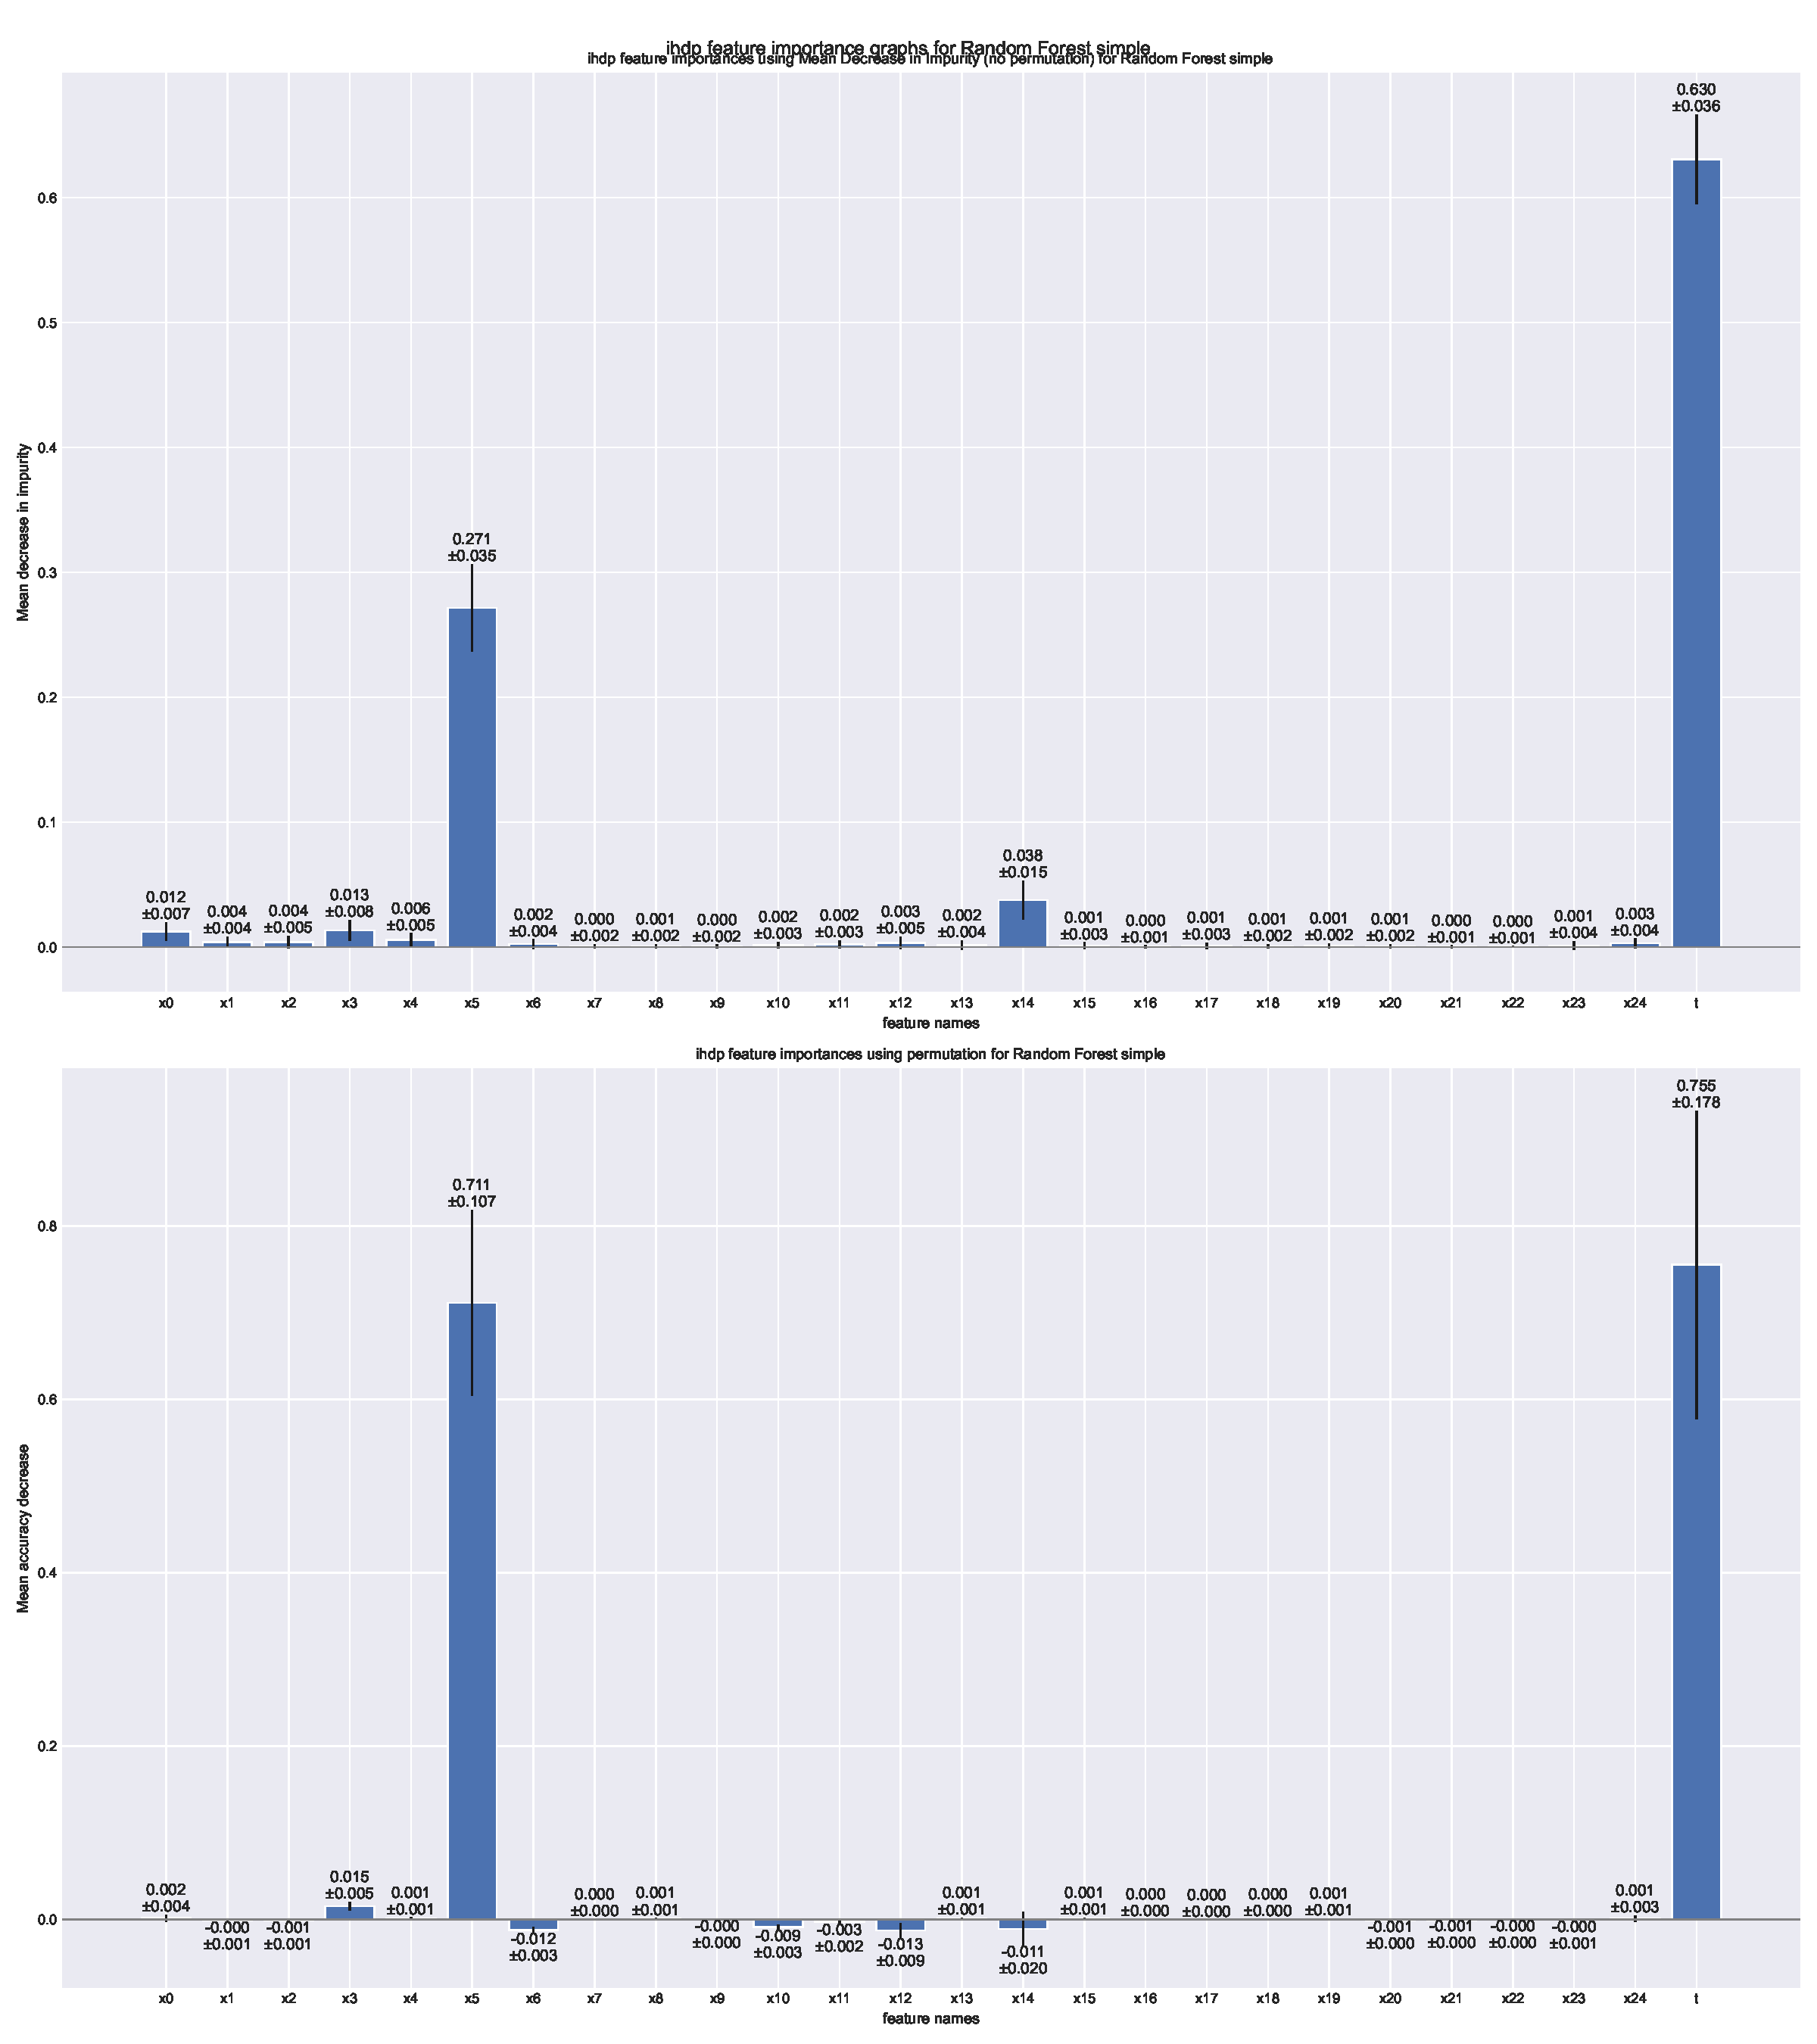
\includegraphics[width=1\linewidth]{project/assignment2/ihdp/ihdp Random Forest simple feature importances.pdf}
  \caption{Feature importances (from feature\_importances\_ and permutation\_test) for IHDP simple RandomForest}
  \label{fig:ihdpSimpleA}
\end{subfigure}%
\begin{subfigure}{.5\textwidth}
  \centering
  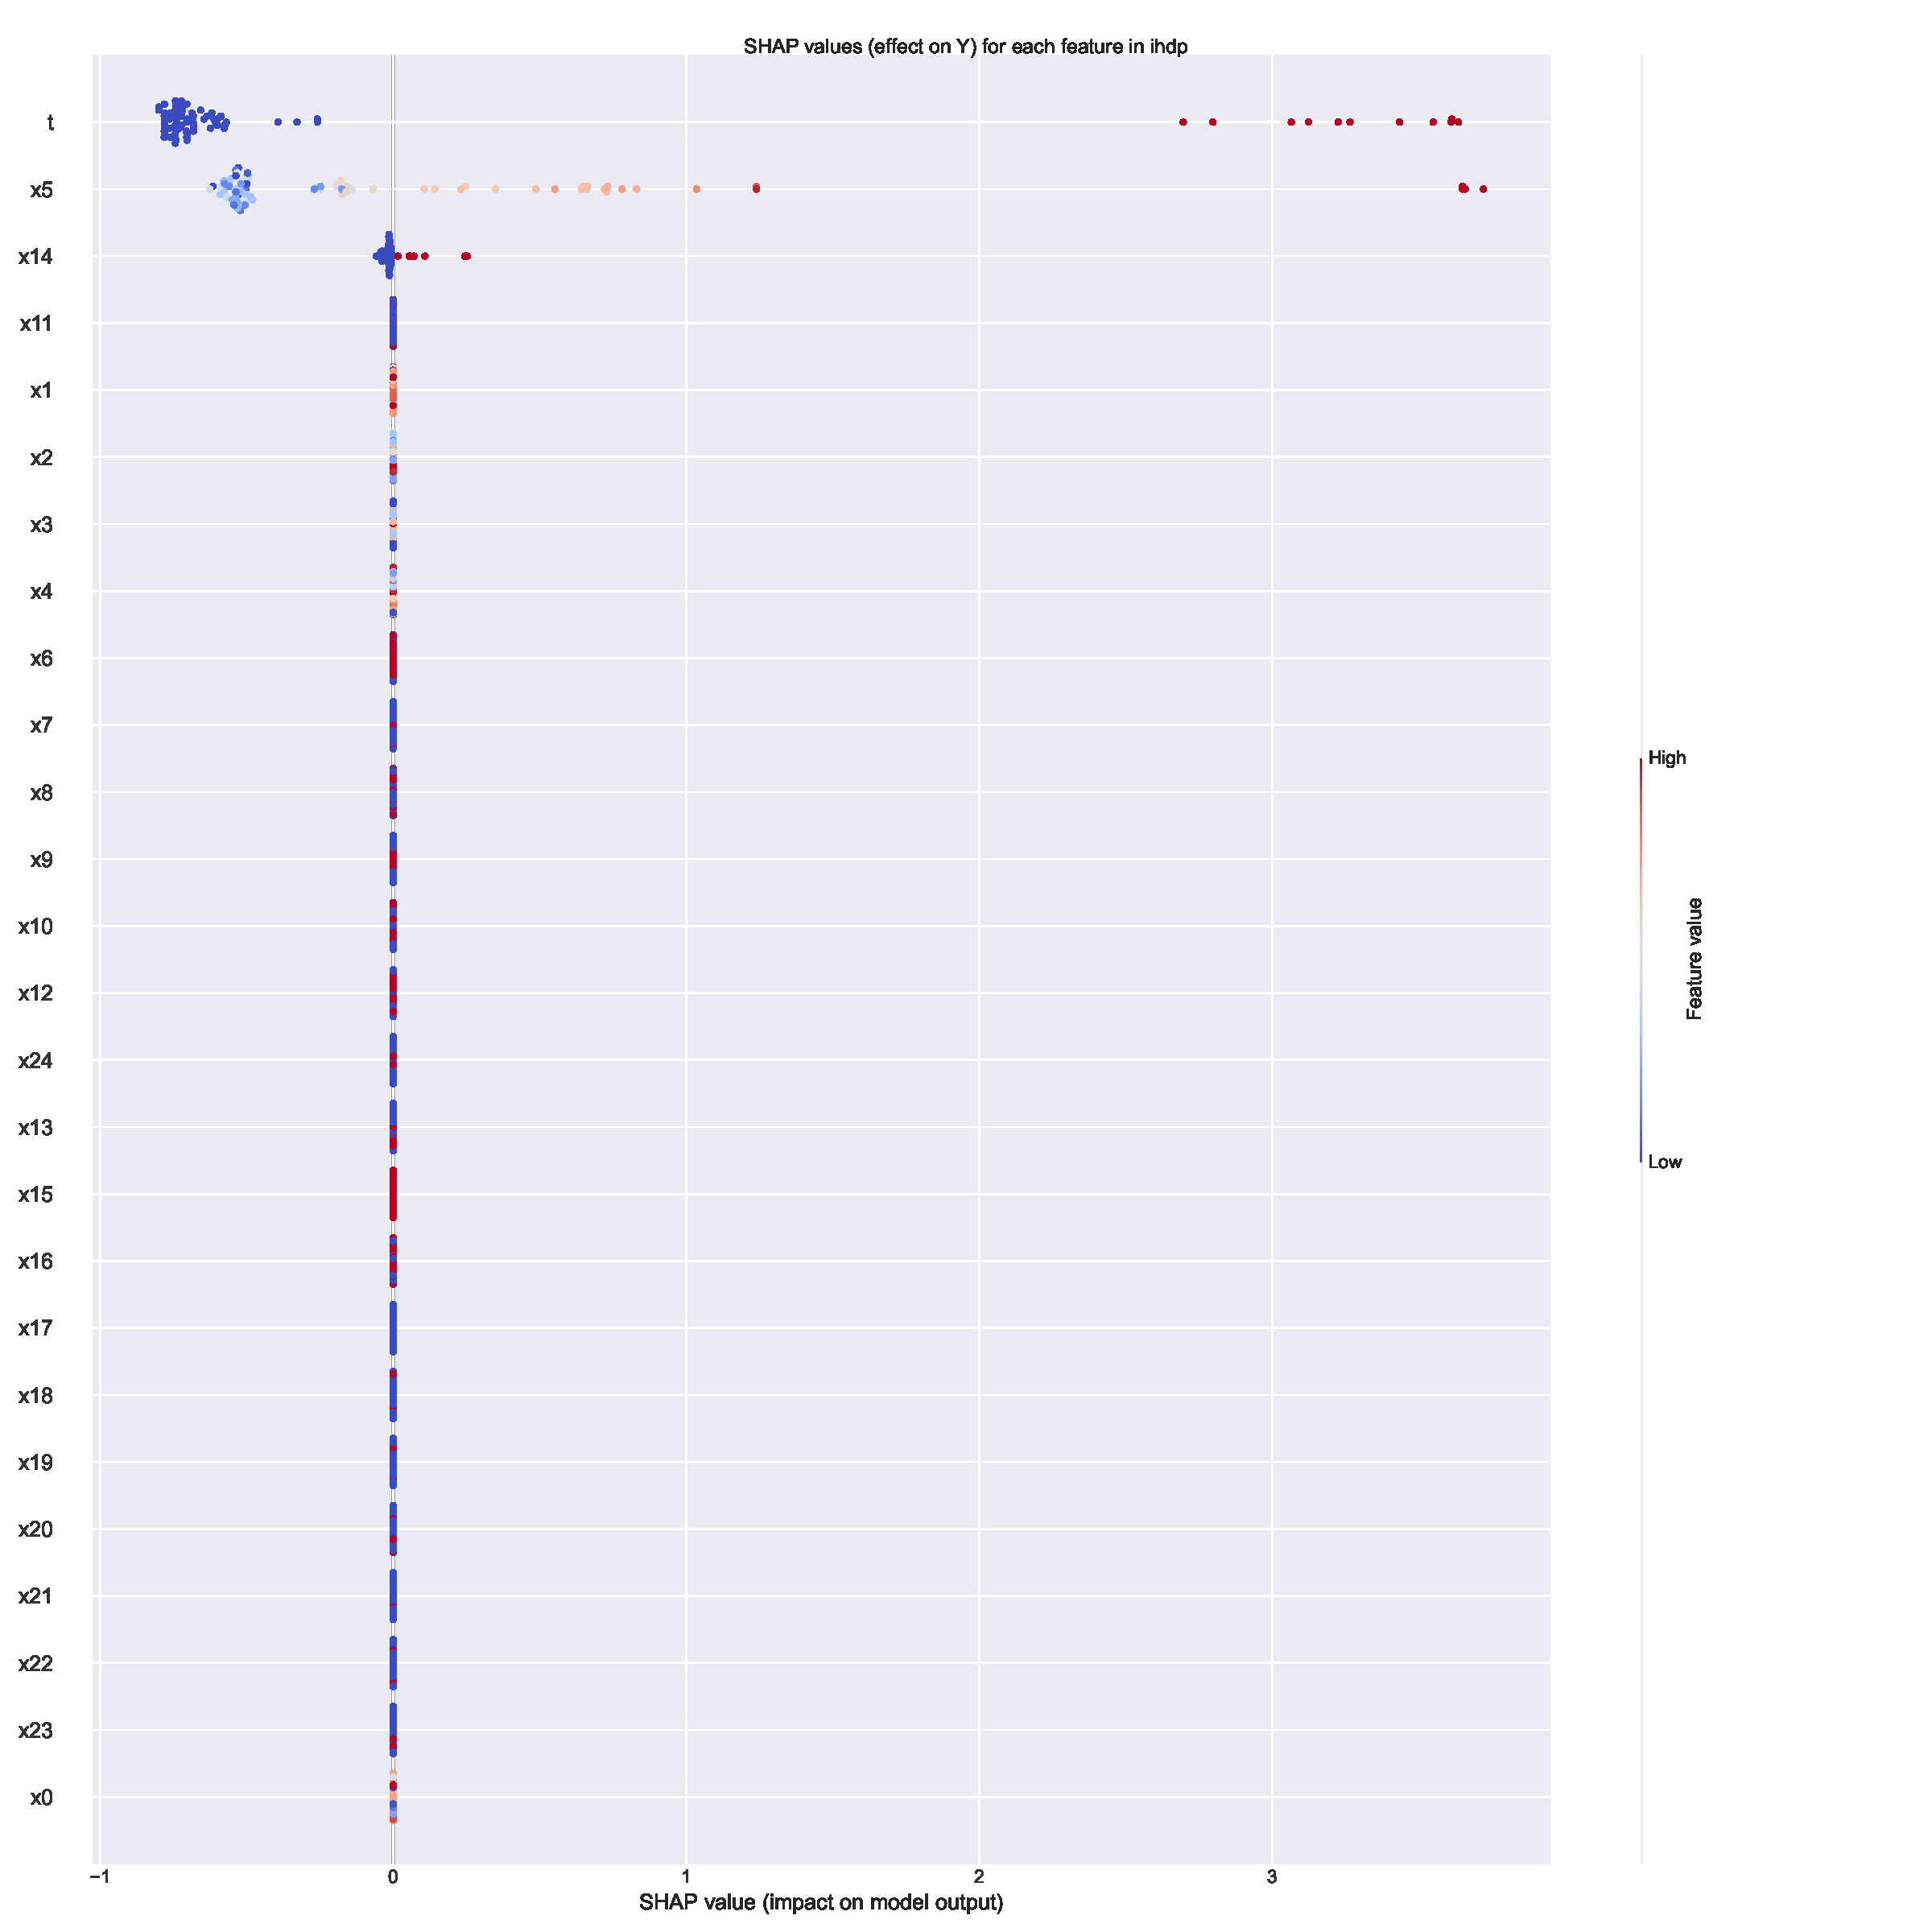
\includegraphics[width=1\linewidth]{project/assignment2/ihdp/ihdp SHAP values for Random Forest simple.pdf}
  \caption{Shapley values for the features as found by the IHDP Y|XT RandomForest predictor}
  \label{fig:ihdpSimpleB}
\end{subfigure}
\caption{Feature importances found by the IHDP Y|XT learner}
\label{fig:ihdpSimple}
\small
Looking at Figure \ref{fig:ihdpSimpleB}, `t=0` has a somewhat negative
impact on the outcome, dwarfed by the positive effect of `t=1`. `x5` has a less
obvious boundary for when the impacts turn positive, however, higher `x5` results in a higher `y`,
whilst a lower `x5` results in a somewhat lower `y`, but the negative effects are less dramatic than
the positives. `x14` appears to have no/negligibly negative impact on `y` when `x14=0`. 
(x14 is a binary value (only 0 or 1), so blue=0, red=1, with potential for a slightly less negligible positive impact when `x14=1`.)
\end{figure}

\FloatBarrier

\subsubsection{IPSW learners (T given X)}

\FloatBarrier

The best estimator for `T|X` for `IHDP` was the SGD classifier, with a
`ROC AUC`\footnote{Receiver Operator Characteristic Area Under Curve} score of 0.71 on the test set.
The feature importances of this classifier (Figure \ref{fig:ihdpIPSW}) appear to be completely different 
to the IHDP `Y|XT` regressor,
with `x5` and `x14` having rather low importances, whilst several other features all compete to have
the highest importance, with wildly fluctuating standard deviations for the importance predictions
visible in Subfigure \ref{fig:ihdpIPSWA}. 

The shapley values (Subfigure \ref{fig:ihdpIPSWB}) are somewhat more coherent;
for all of the binary features, values of `0` and `1` have
opposing impacts on the final `t` value\footnote{By this, I mean that 'for the ones where xN=0 has a negative effect, xN=1 has a positive effect, and vice versa'}. The continuous values are a bit more
fuzzy in this regard, but they mostly follow this rule of 'bigger has opposite sign effect to smaller'.
The only real exception is with `x3`; the high and slightly low values of `x3` have negative impacts,
and only the particularly small `x3` values have a positive impact.

Considering this unusual overlap, the rather high importance granted to `x3` in
Subfigure \ref{fig:ihdpIPSWA}, and the fact that children with a birth weight above 2500g were not
eligible for inclusion in the treatment group in the `IHDP` study \cite{Gross1993}, this suggests that
`x3` might indicate 'birth weight'\footnote{With the higher x3 values resulting in a lower t due to the ineligibility for treatment. Then again, this is just conjecture}.

\begin{figure}[H]
\centering
\begin{subfigure}{.5\textwidth}
  \centering
  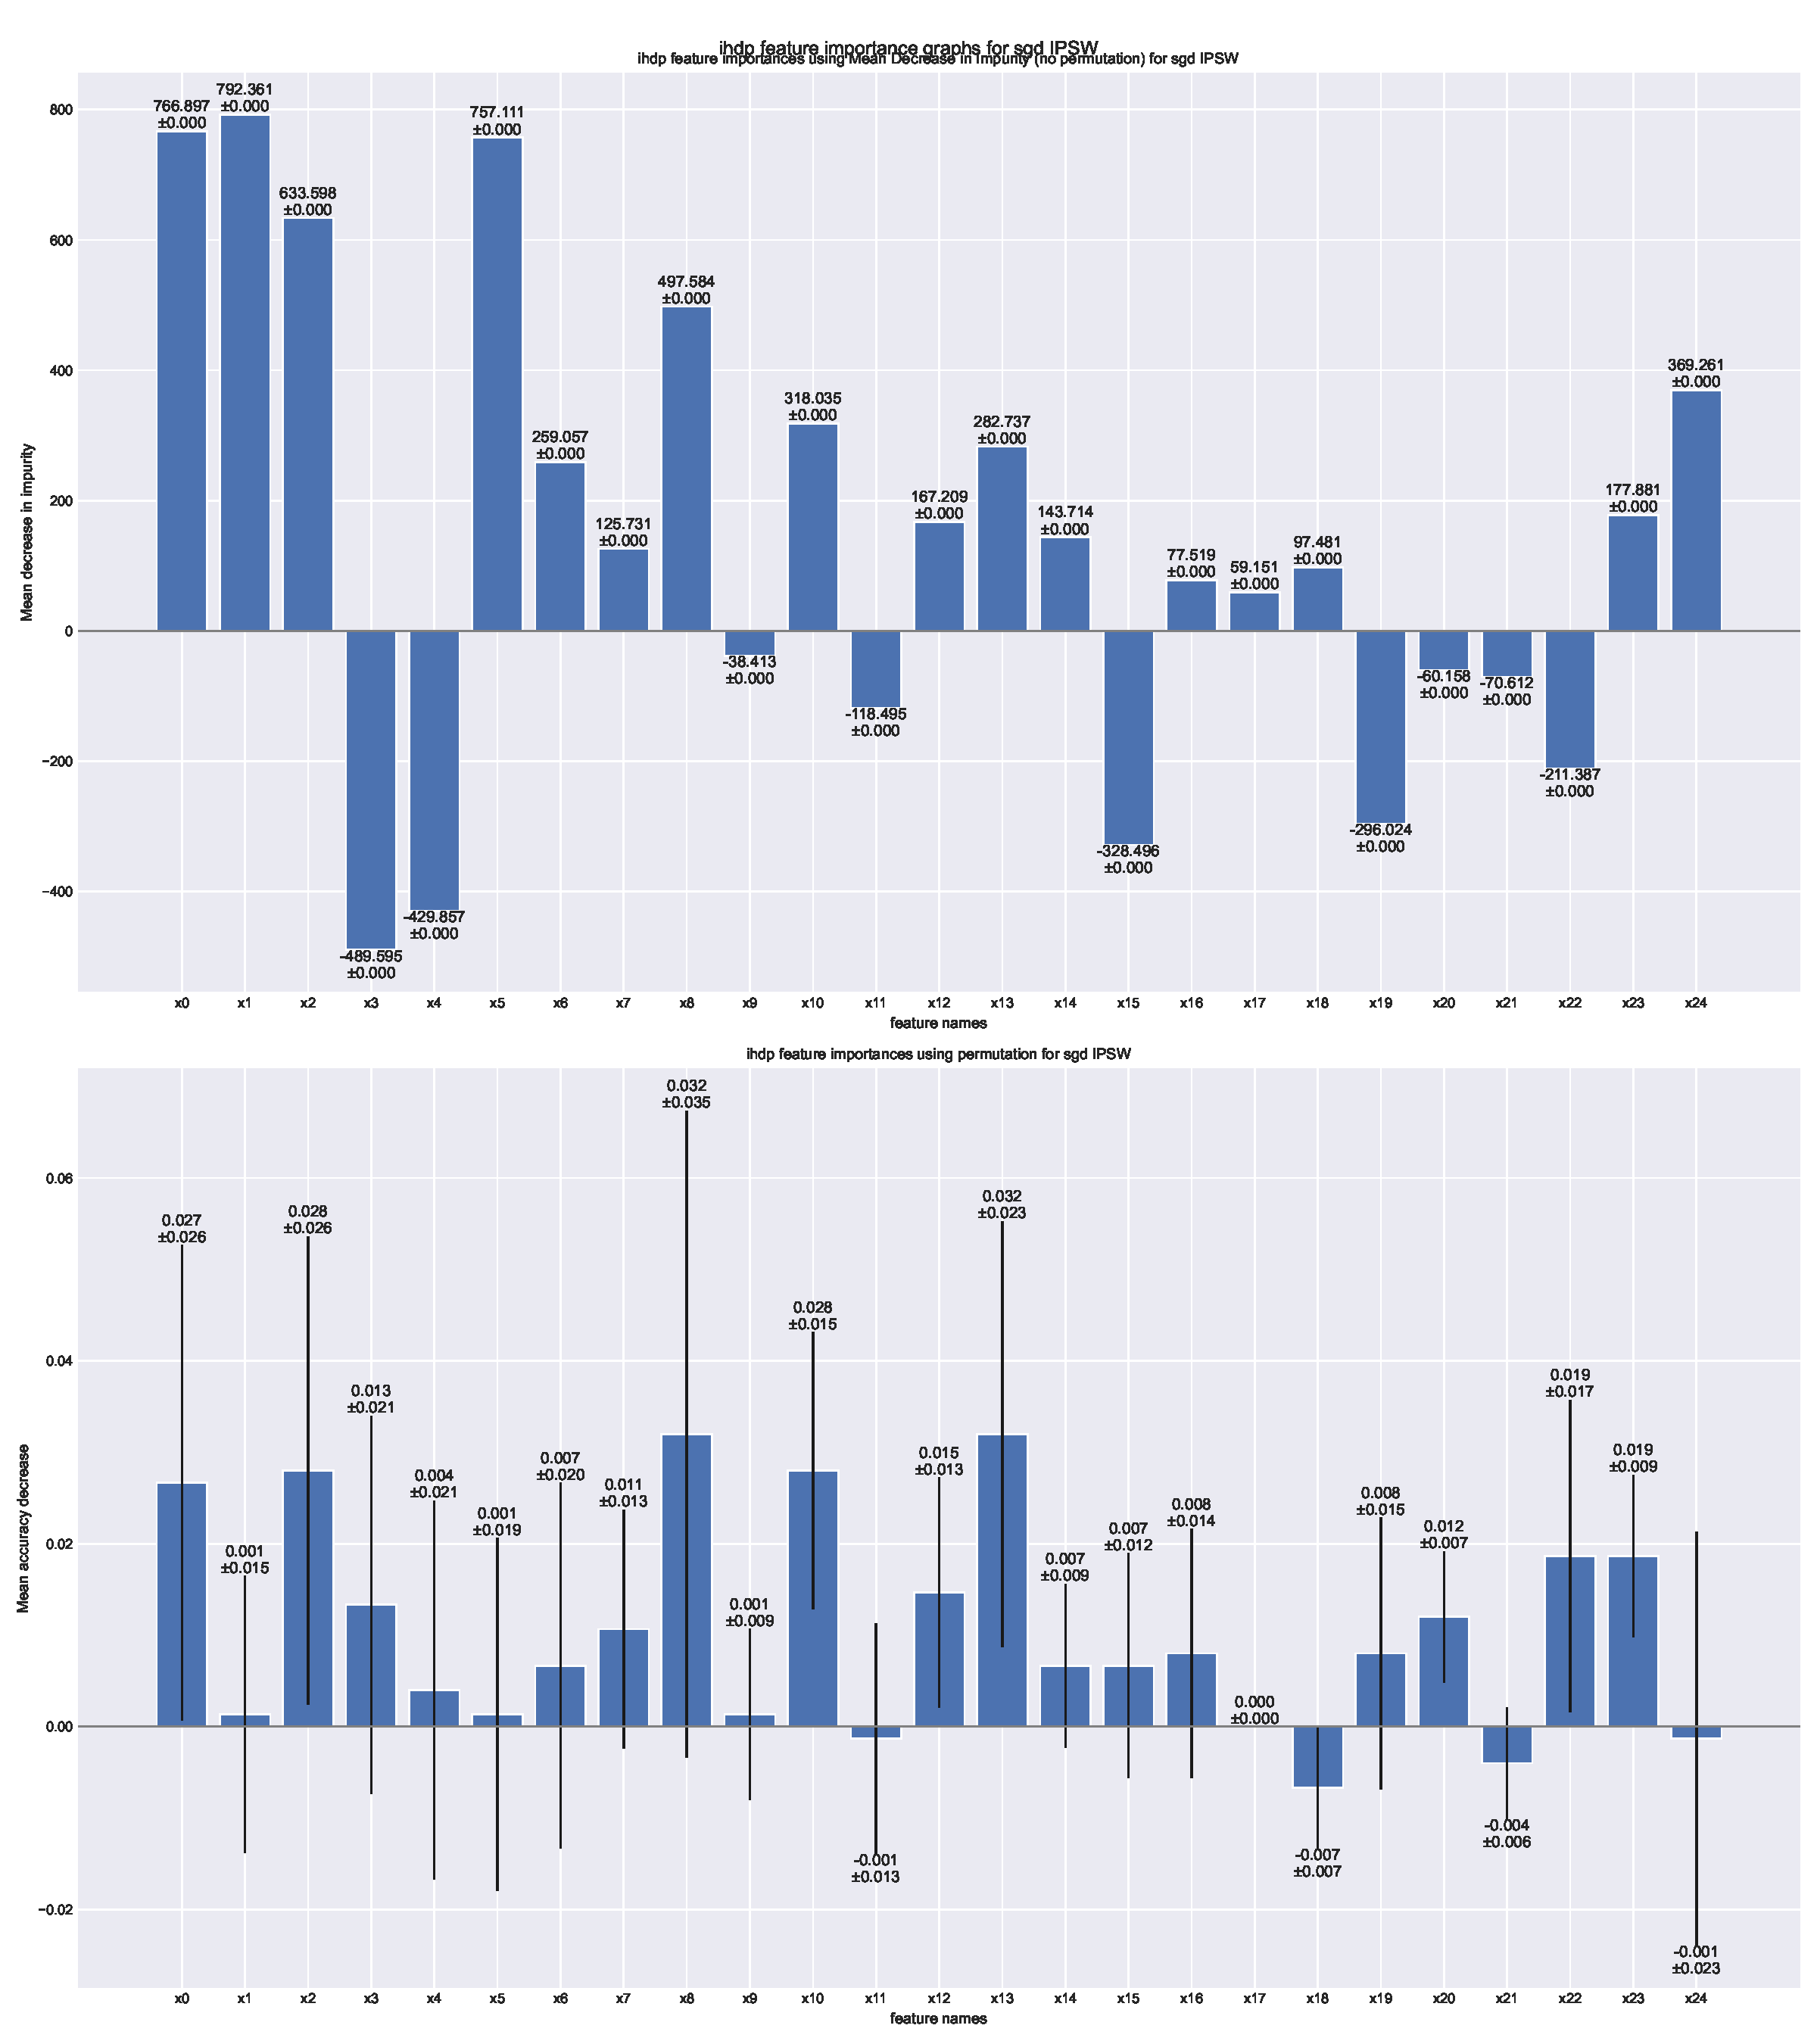
\includegraphics[width=1\linewidth]{project/assignment2/ihdp/ihdp SGD IPSW feature importances.pdf}
  \caption{Feature importances (from feature\_importances\_ and permutation\_test) for IHDP IPSW SGD}
  \label{fig:ihdpIPSWA}
\end{subfigure}%
\begin{subfigure}{.5\textwidth}
  \centering
  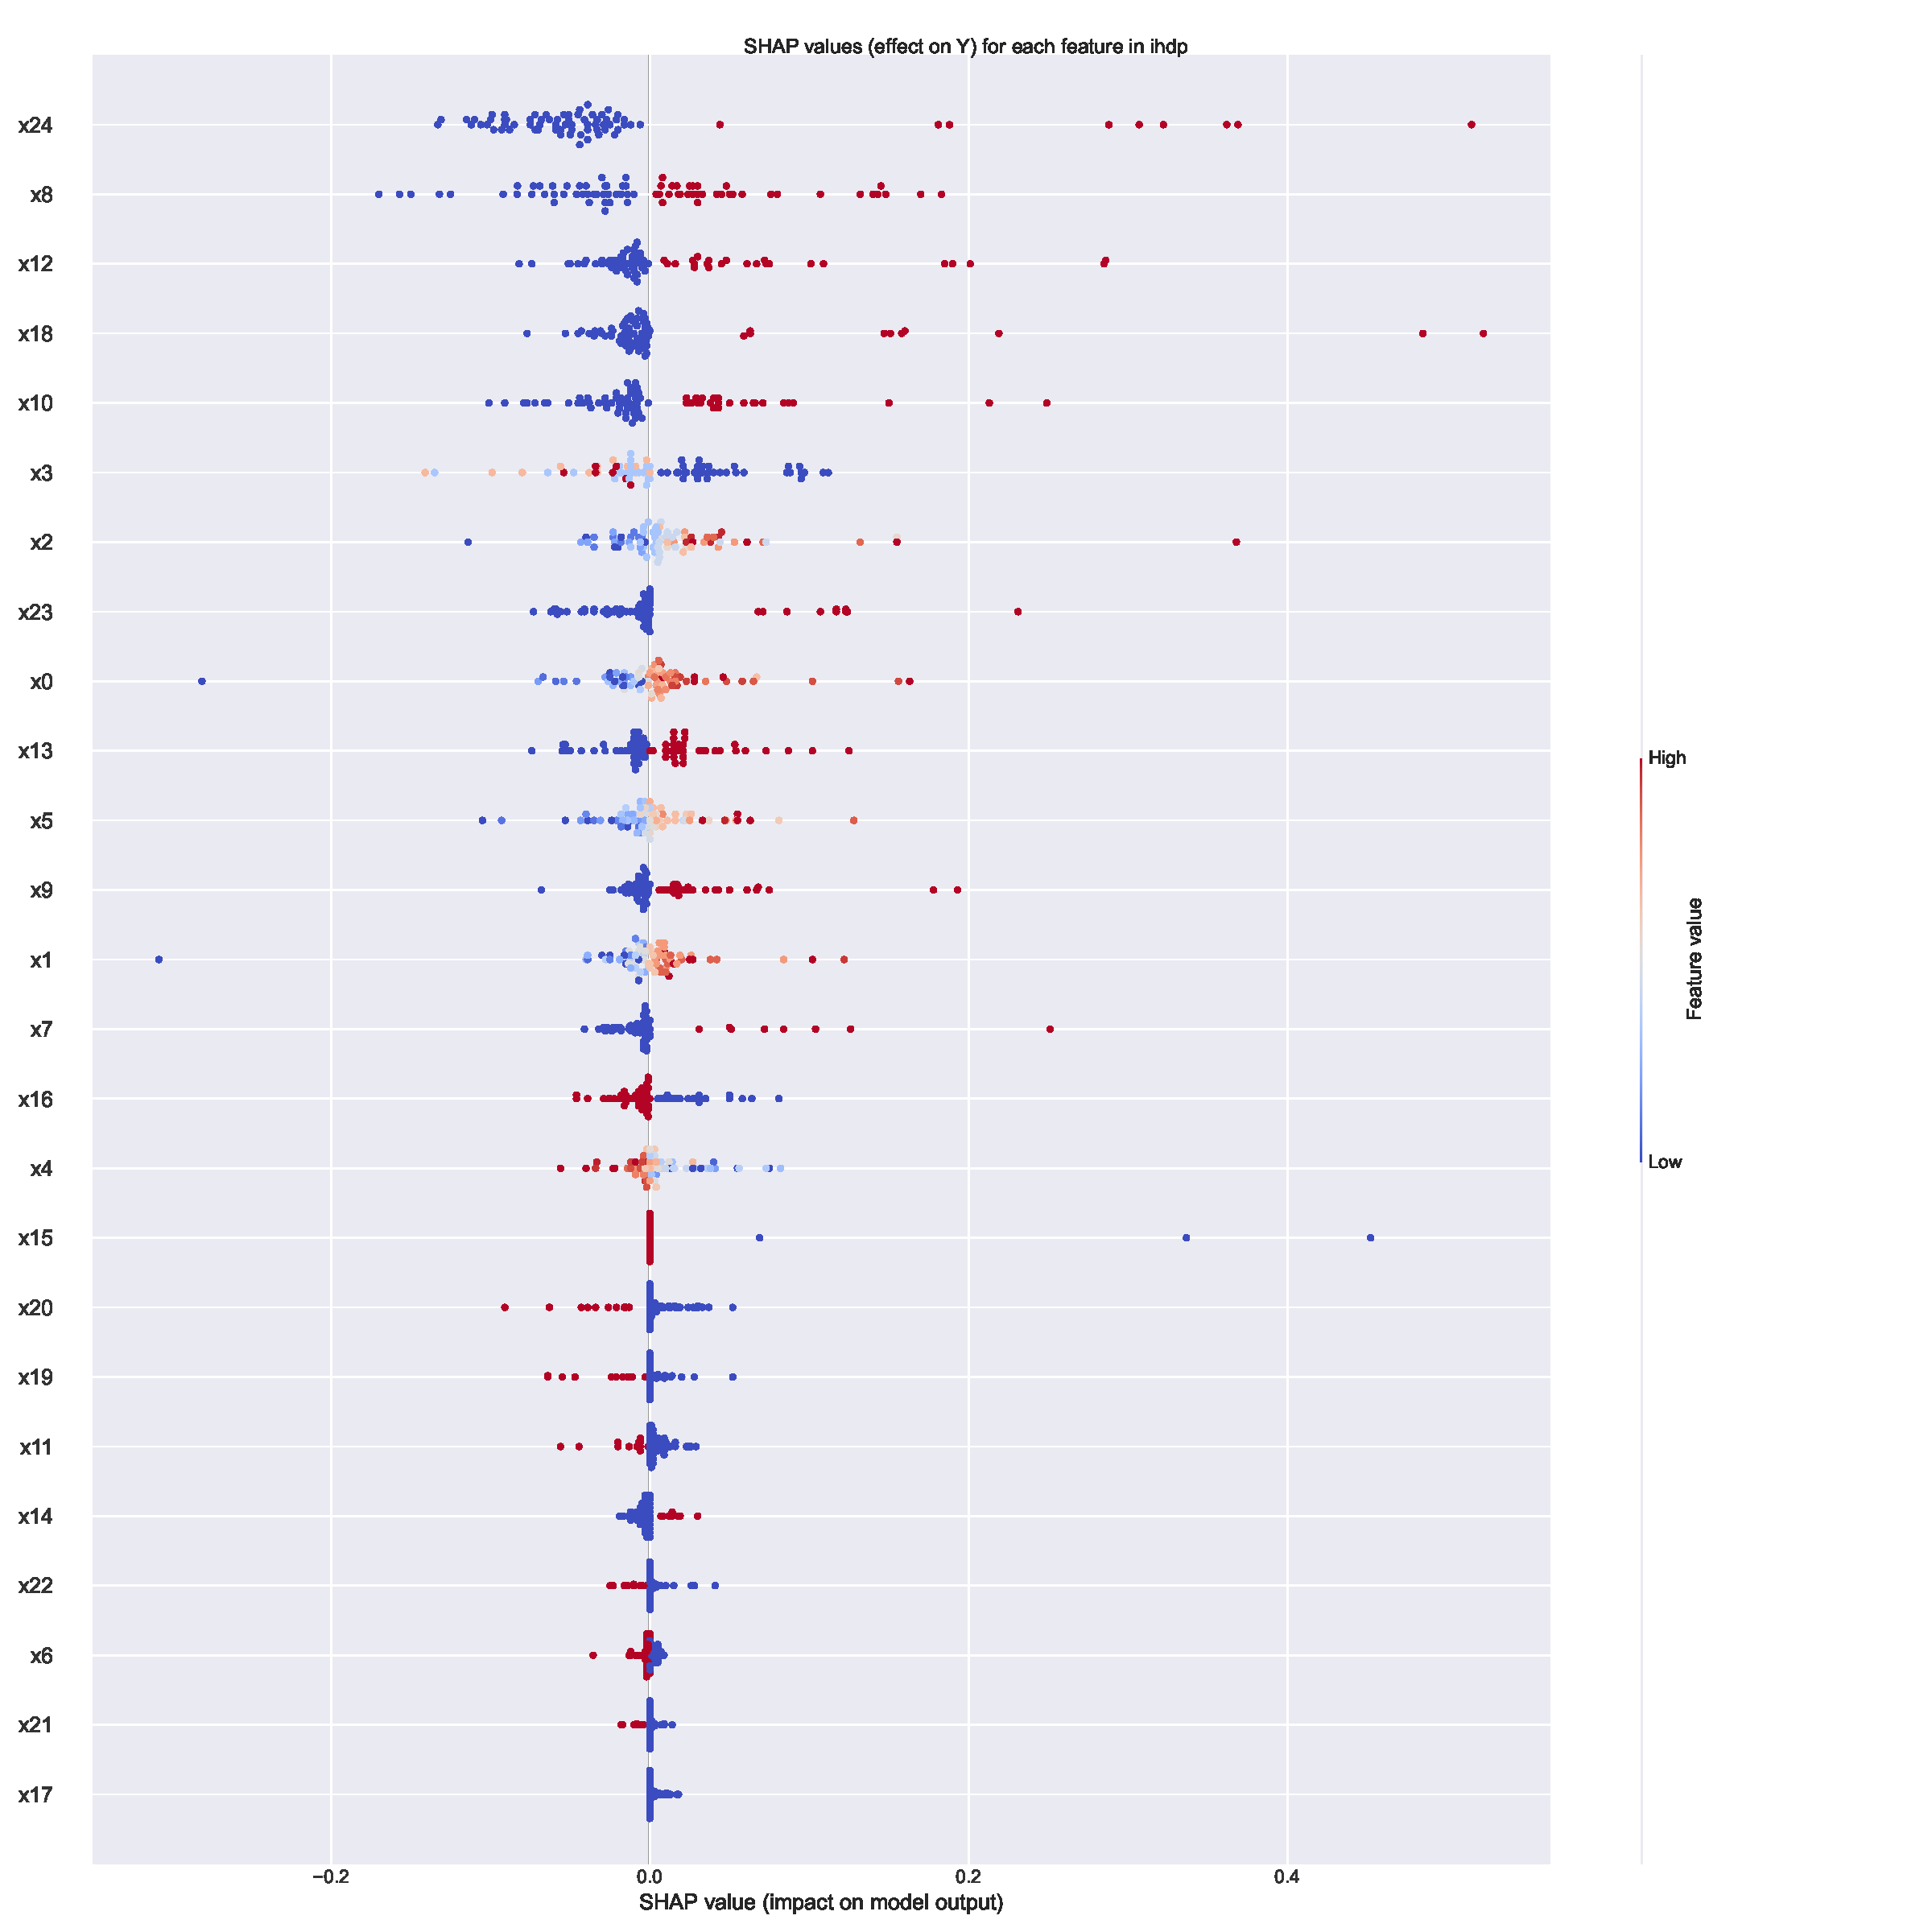
\includegraphics[width=1\linewidth]{project/assignment2/ihdp/ihdp SHAP values for sgd IPSW.pdf}
  \caption{Shapley values for the features as found by the IHDP T|X SGD predictor}
  \label{fig:ihdpIPSWB}
\end{subfigure}
\caption{Feature importances found by the IHDP T|X learner}
\label{fig:ihdpIPSW}
\end{figure}

\FloatBarrier


\subsubsection{IHDP simple learners with IPSW (Y given XT*IPSW(X))}

\FloatBarrier

Once again, the `RandomForestRegressor` had the best result (`r2` score of 0.70), and, once again,
as shown in Figure \ref{fig:ihdpSimpleIPSW}, `t` is the most important feature, followed by `x5`,
`x14` is questionably important\footnote{The estimator's 'feature\_importances\_' property gave it a somewhat positive result, but scikit-learn's 'permutation\_test' functionality gave it a mostly negative result, but the shapley values still indicate some significance}, and then everything else being almost entirely unimportant.


\begin{figure}[H]
\centering
\begin{subfigure}{.5\textwidth}
  \centering
  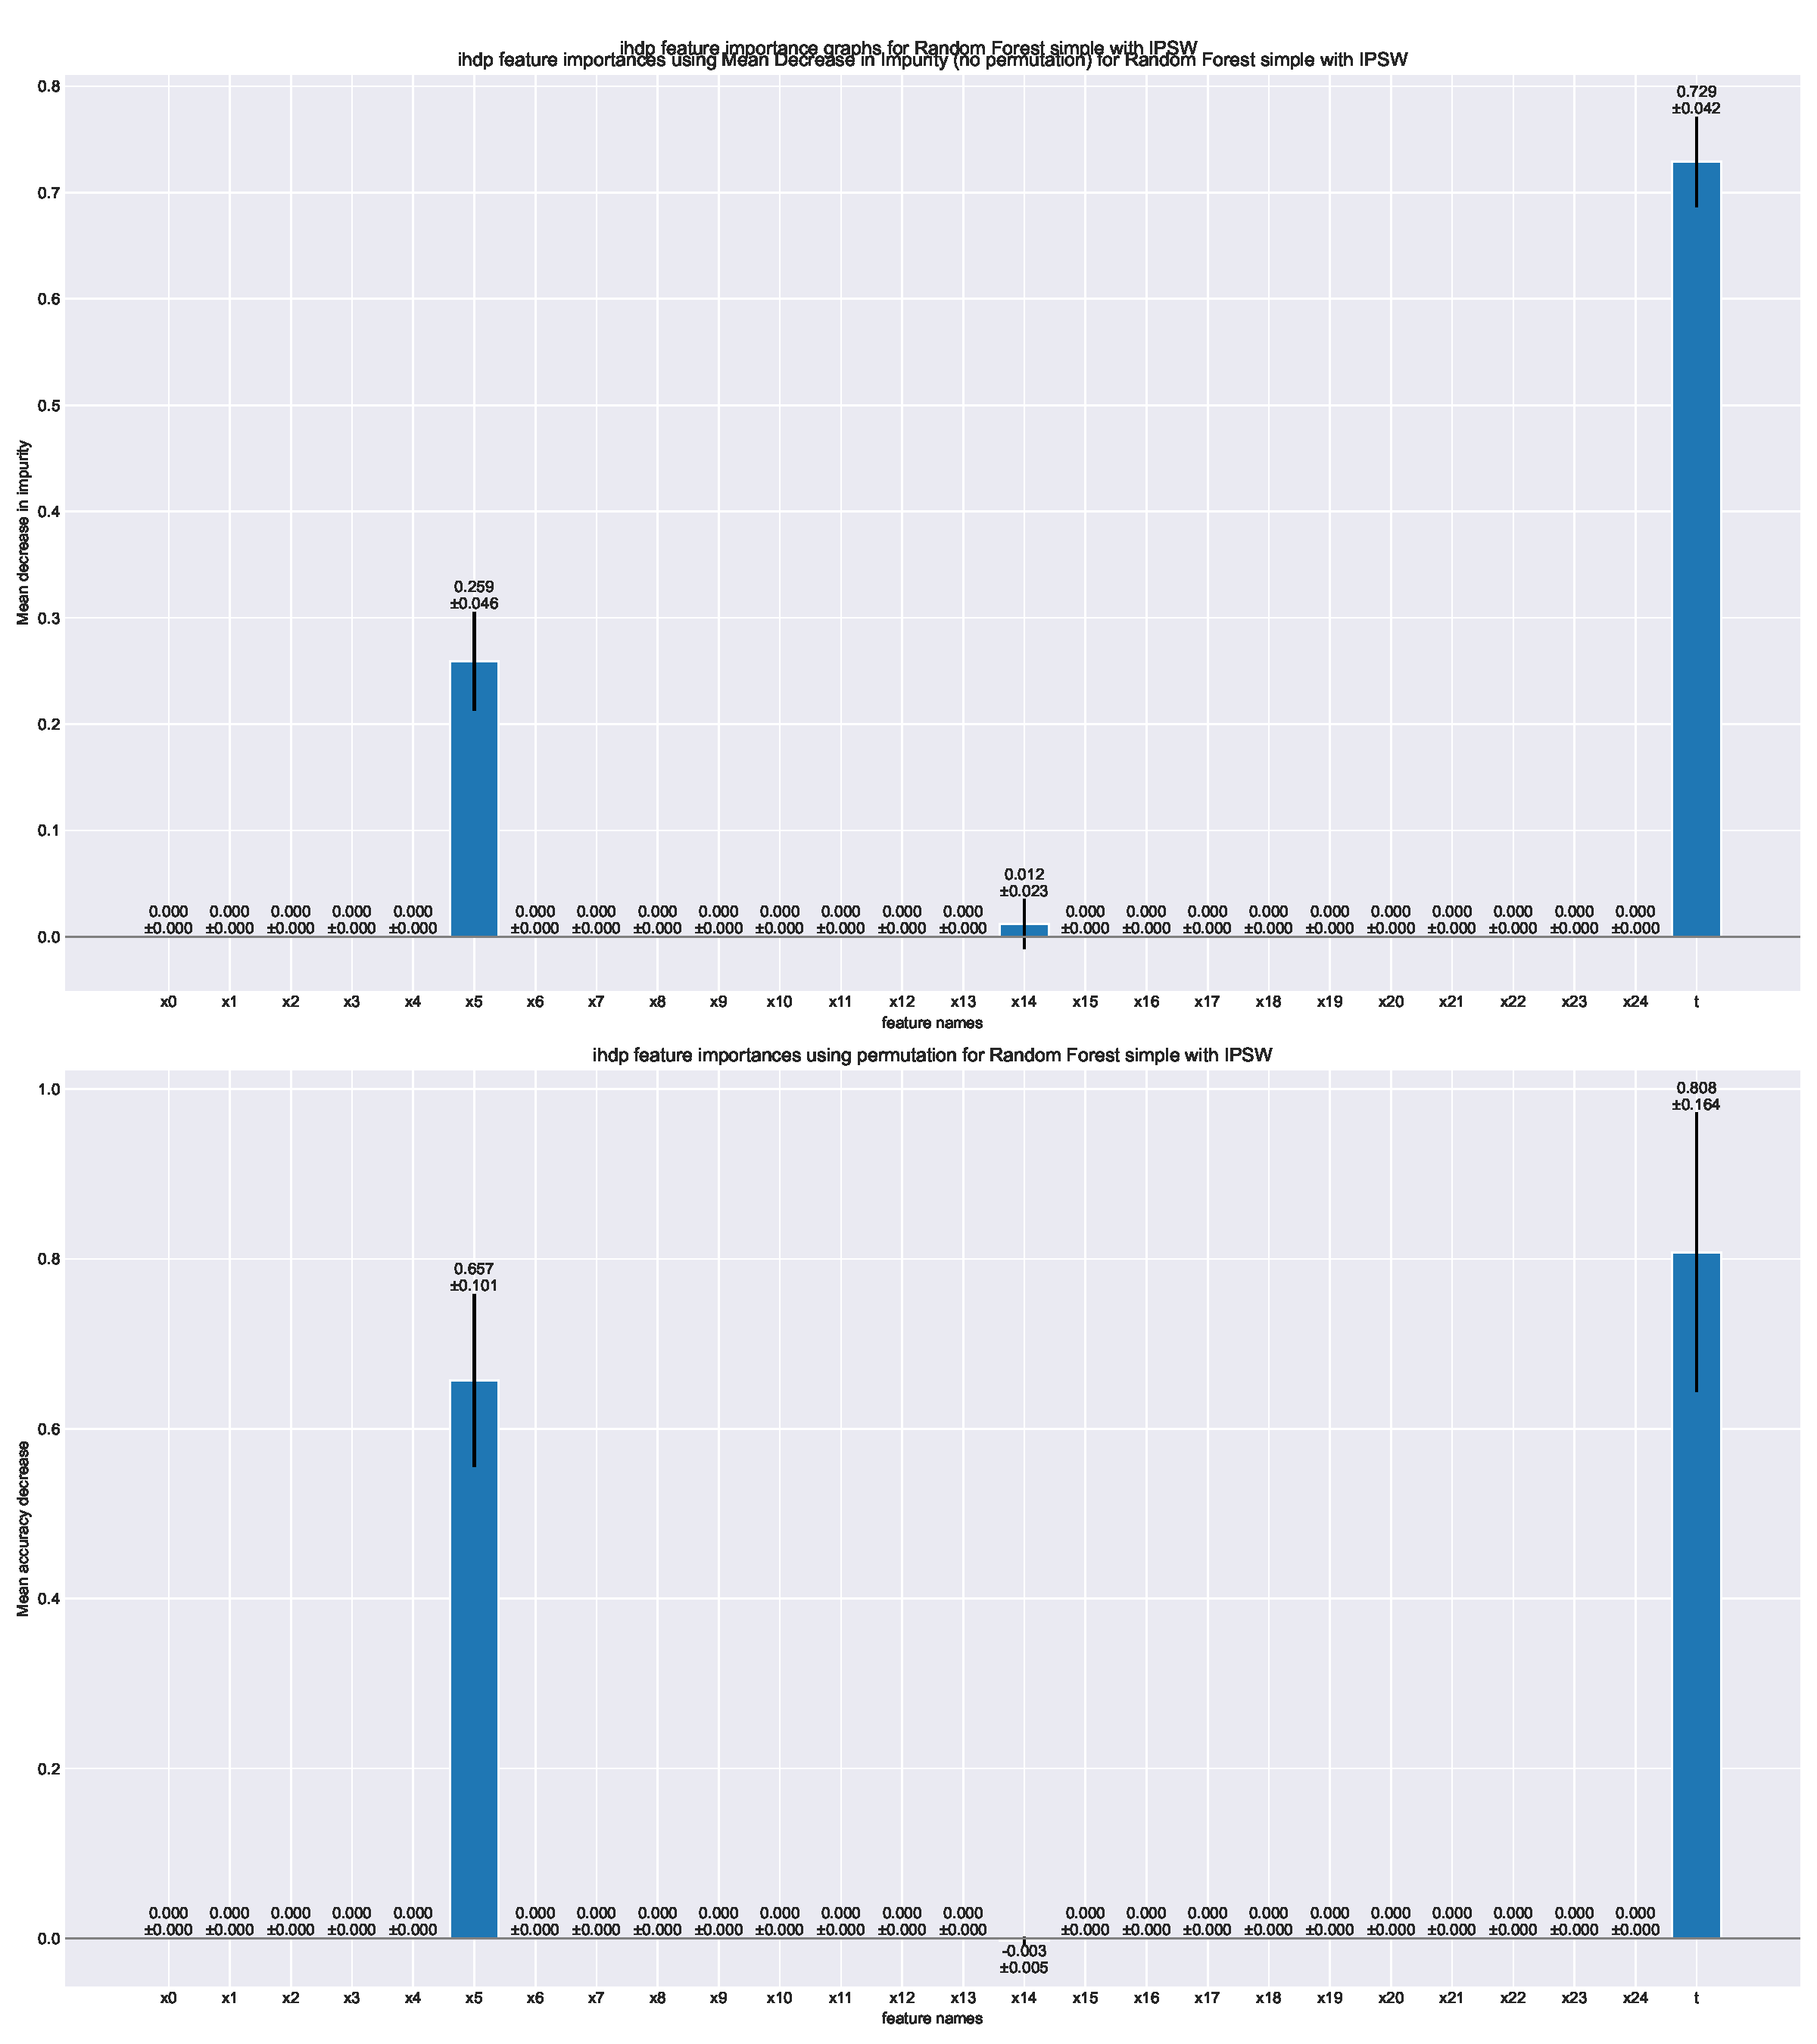
\includegraphics[width=1\linewidth]{project/assignment2/ihdp/ihdp Random Forest simple with IPSW feature importances.pdf}
  \caption{Feature importances (from feature\_importances\_ and permutation\_test) for IHDP simple+IPSW RandomForest}
  \label{fig:ihdpSimpleIPSWA}
\end{subfigure}%
\begin{subfigure}{.5\textwidth}
  \centering
  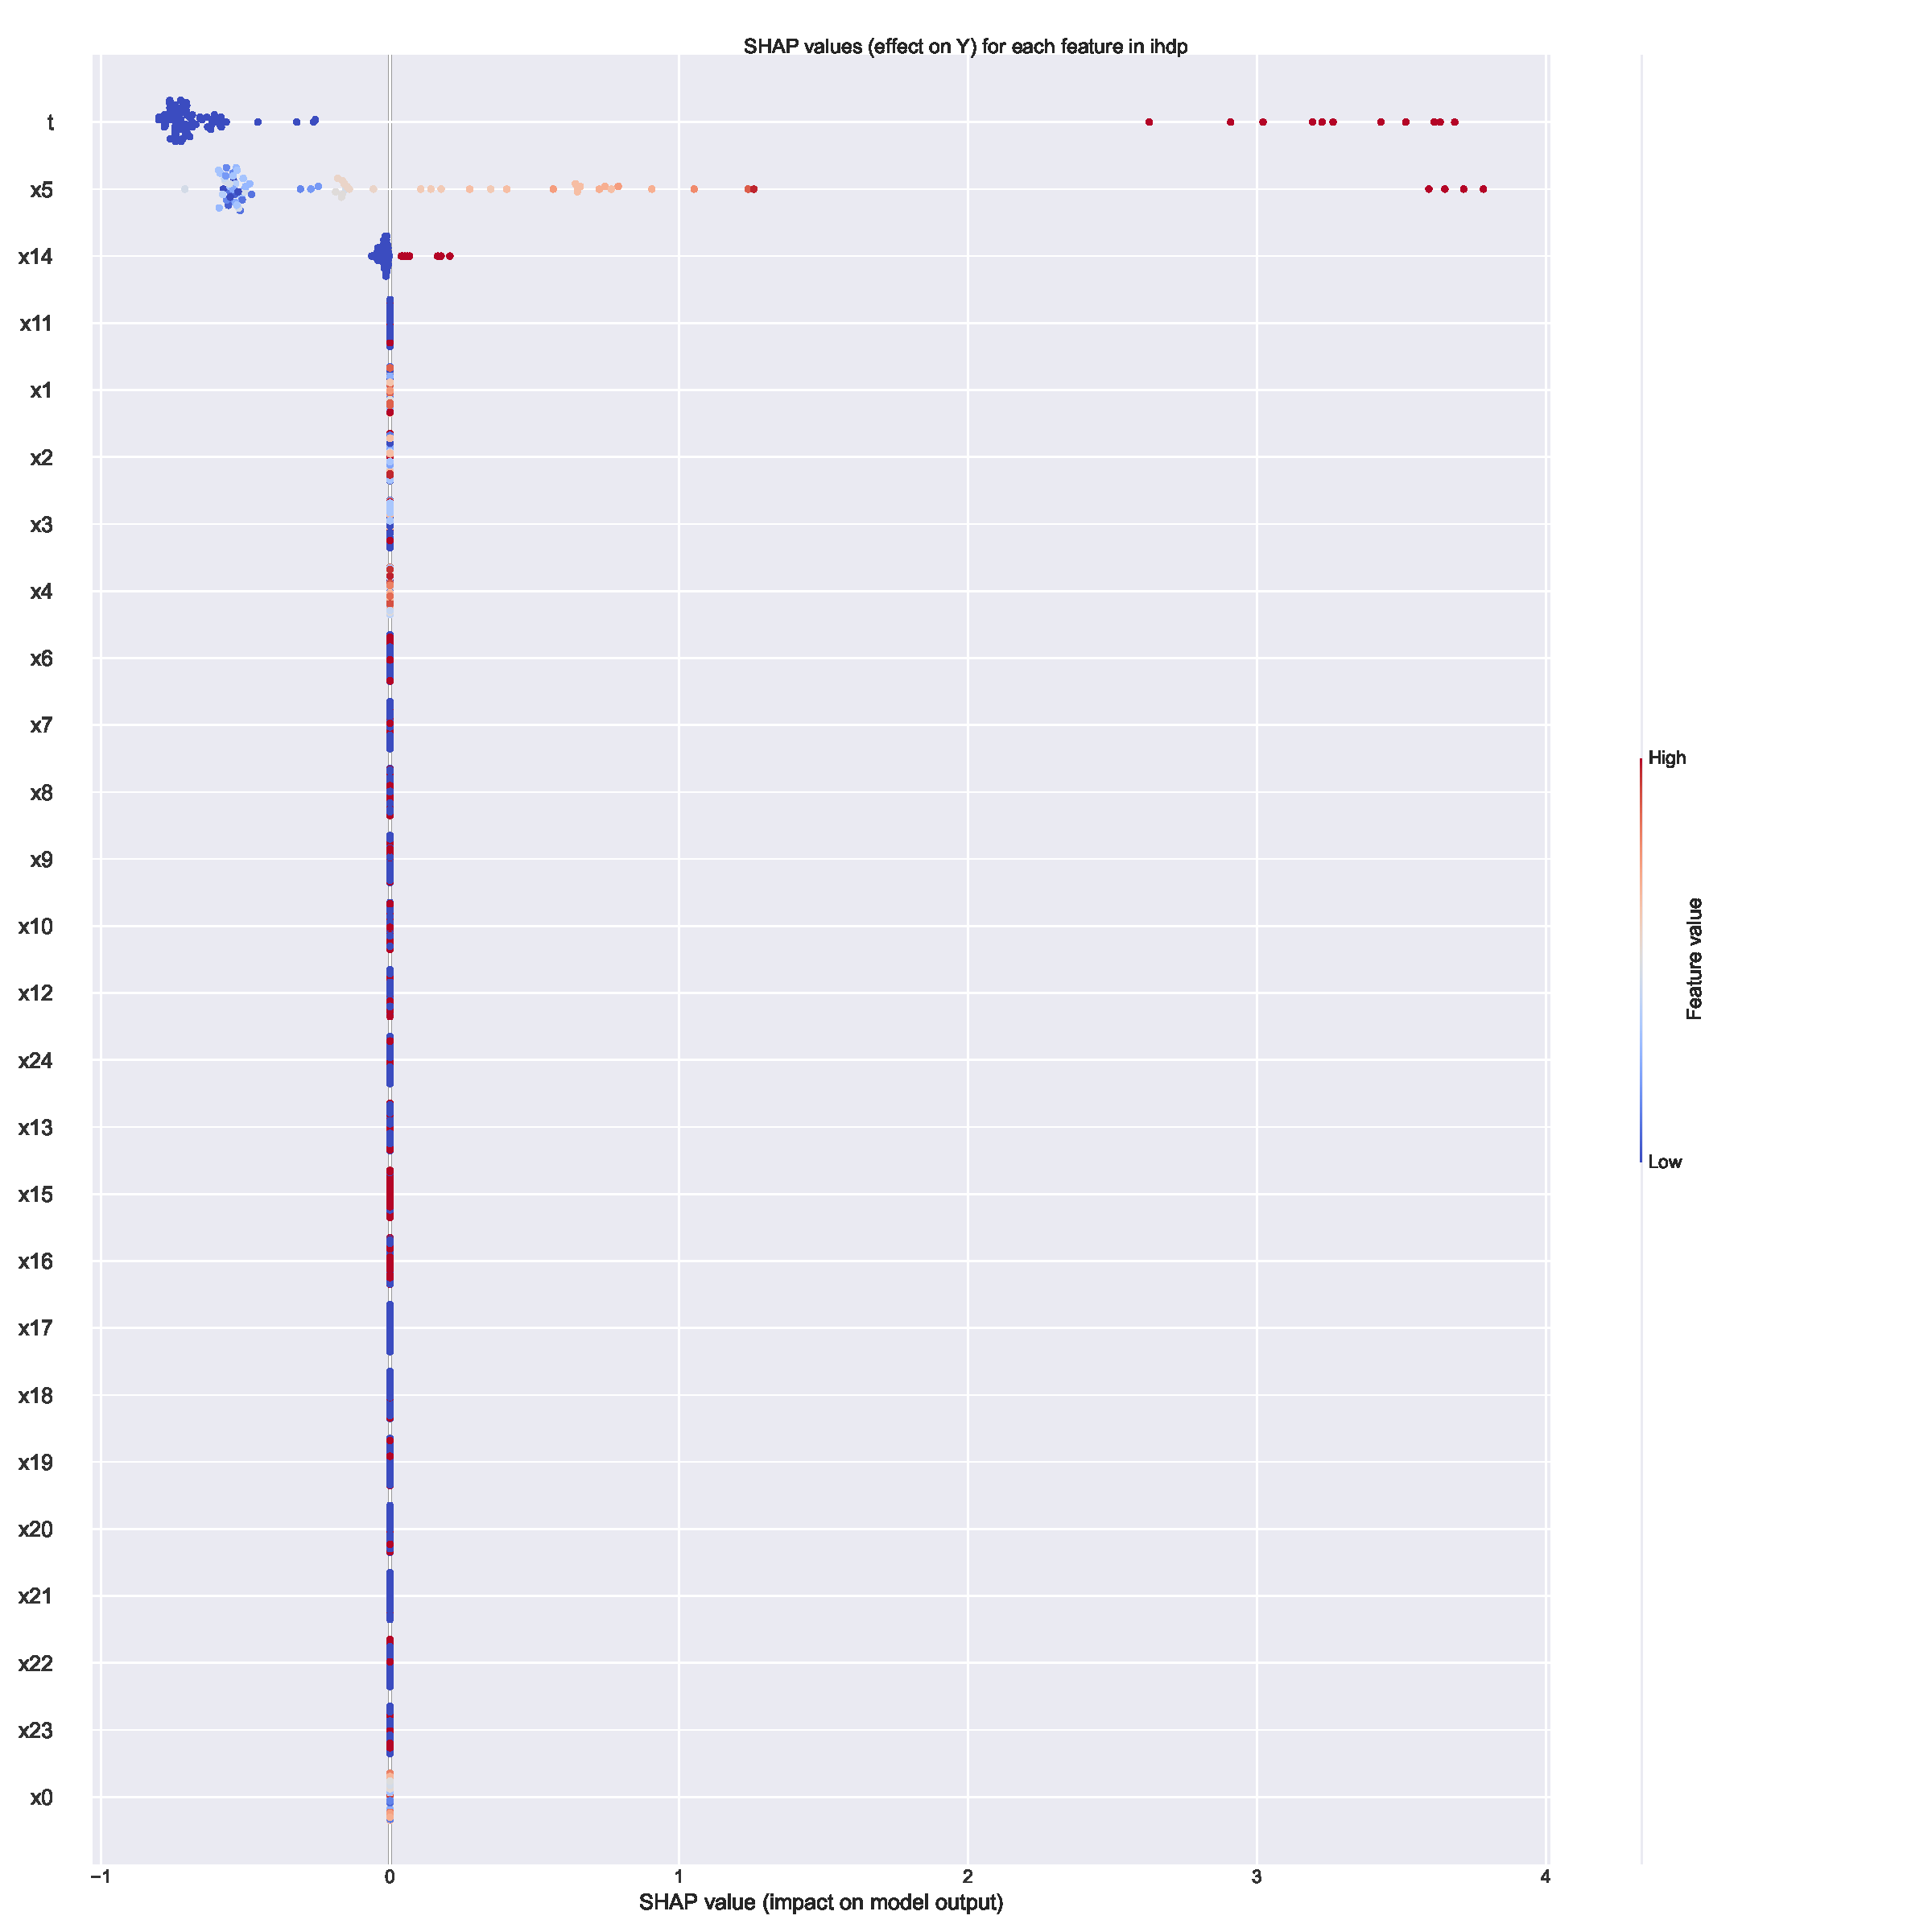
\includegraphics[width=1\linewidth]{project/assignment2/ihdp/ihdp SHAP values for Random Forest simple with IPSW.pdf}
  \caption{Shapley values for the features as found by the IHDP Y|XT*IPSW RandomForest predictor}
  \label{fig:ihdpSimpleIPSWB}
\end{subfigure}
\caption{Feature importances found by the IHDP Y|XT*IPSW learner}
\label{fig:ihdpSimpleIPSW}
\small
\justifying
Seeing as the `T|X` predictor, shown in Figure \ref{fig:ihdpIPSW}, was used to help fit this predictor,
I would have assumed that the importances of the inputs to `T` derived from that would have had some 
tangible impact on this learner's importances, but their lack of an impact is somewhat concerning.
This either suggests underfitting, the impacts of `T` effectively outweighing the impacts of the
contributors to `T`, or both. The most probable explanation would likely be underfitting, as the
other 'best' learners (being ARDRegressor, SGDRegressor, and Adaboosted versions of those and RandomForest) all had somewhat more complex importance/shapley graphs, yet lower `r2`
scores (everything but the RandomForest/Adaboosted Random Forest having r2 scores around 0.5),
implying that they overfit to the point of becoming less accurate than this underfit regressor.
\end{figure}

\FloatBarrier

\subsubsection{IHDP CATE estimator}

\FloatBarrier

The best CATE estimator for `IHDP` was the `CausalForestDML` estimator, with a
PEHE\footnote{error in Precision of Estimation of Heterogeneous Effect} value of 4.8.
However, looking at the outputs of it, I suspect that the somewhat underfit models produced in the
previous stage, used as inputs to this model, may have resulted in this model not being fitted correctly
either, resulting in the unusual results visible in Figures \ref{fig:ihdpCATEcfA} and \ref{fig:ihdpCATEcf}.

The shapley values for one of the other CATE models, which more closely resembles what one may have expected
to see considering the inputs so far, can be seen in Figure \ref{fig:ihdpForestDRShap}, although that
other model had an atrocious PEHE score, so that other model may be a case of garbage-in-garbage-out,
with this model ultimately being more accurate overall.

The unexpected shapley values could be due to this model finding out that x2 and x0 were confounders,
however, as the inputs to this model were massively underfit, I cannot confidently assert that to be
the case.

\begin{figure}[H]
\centering
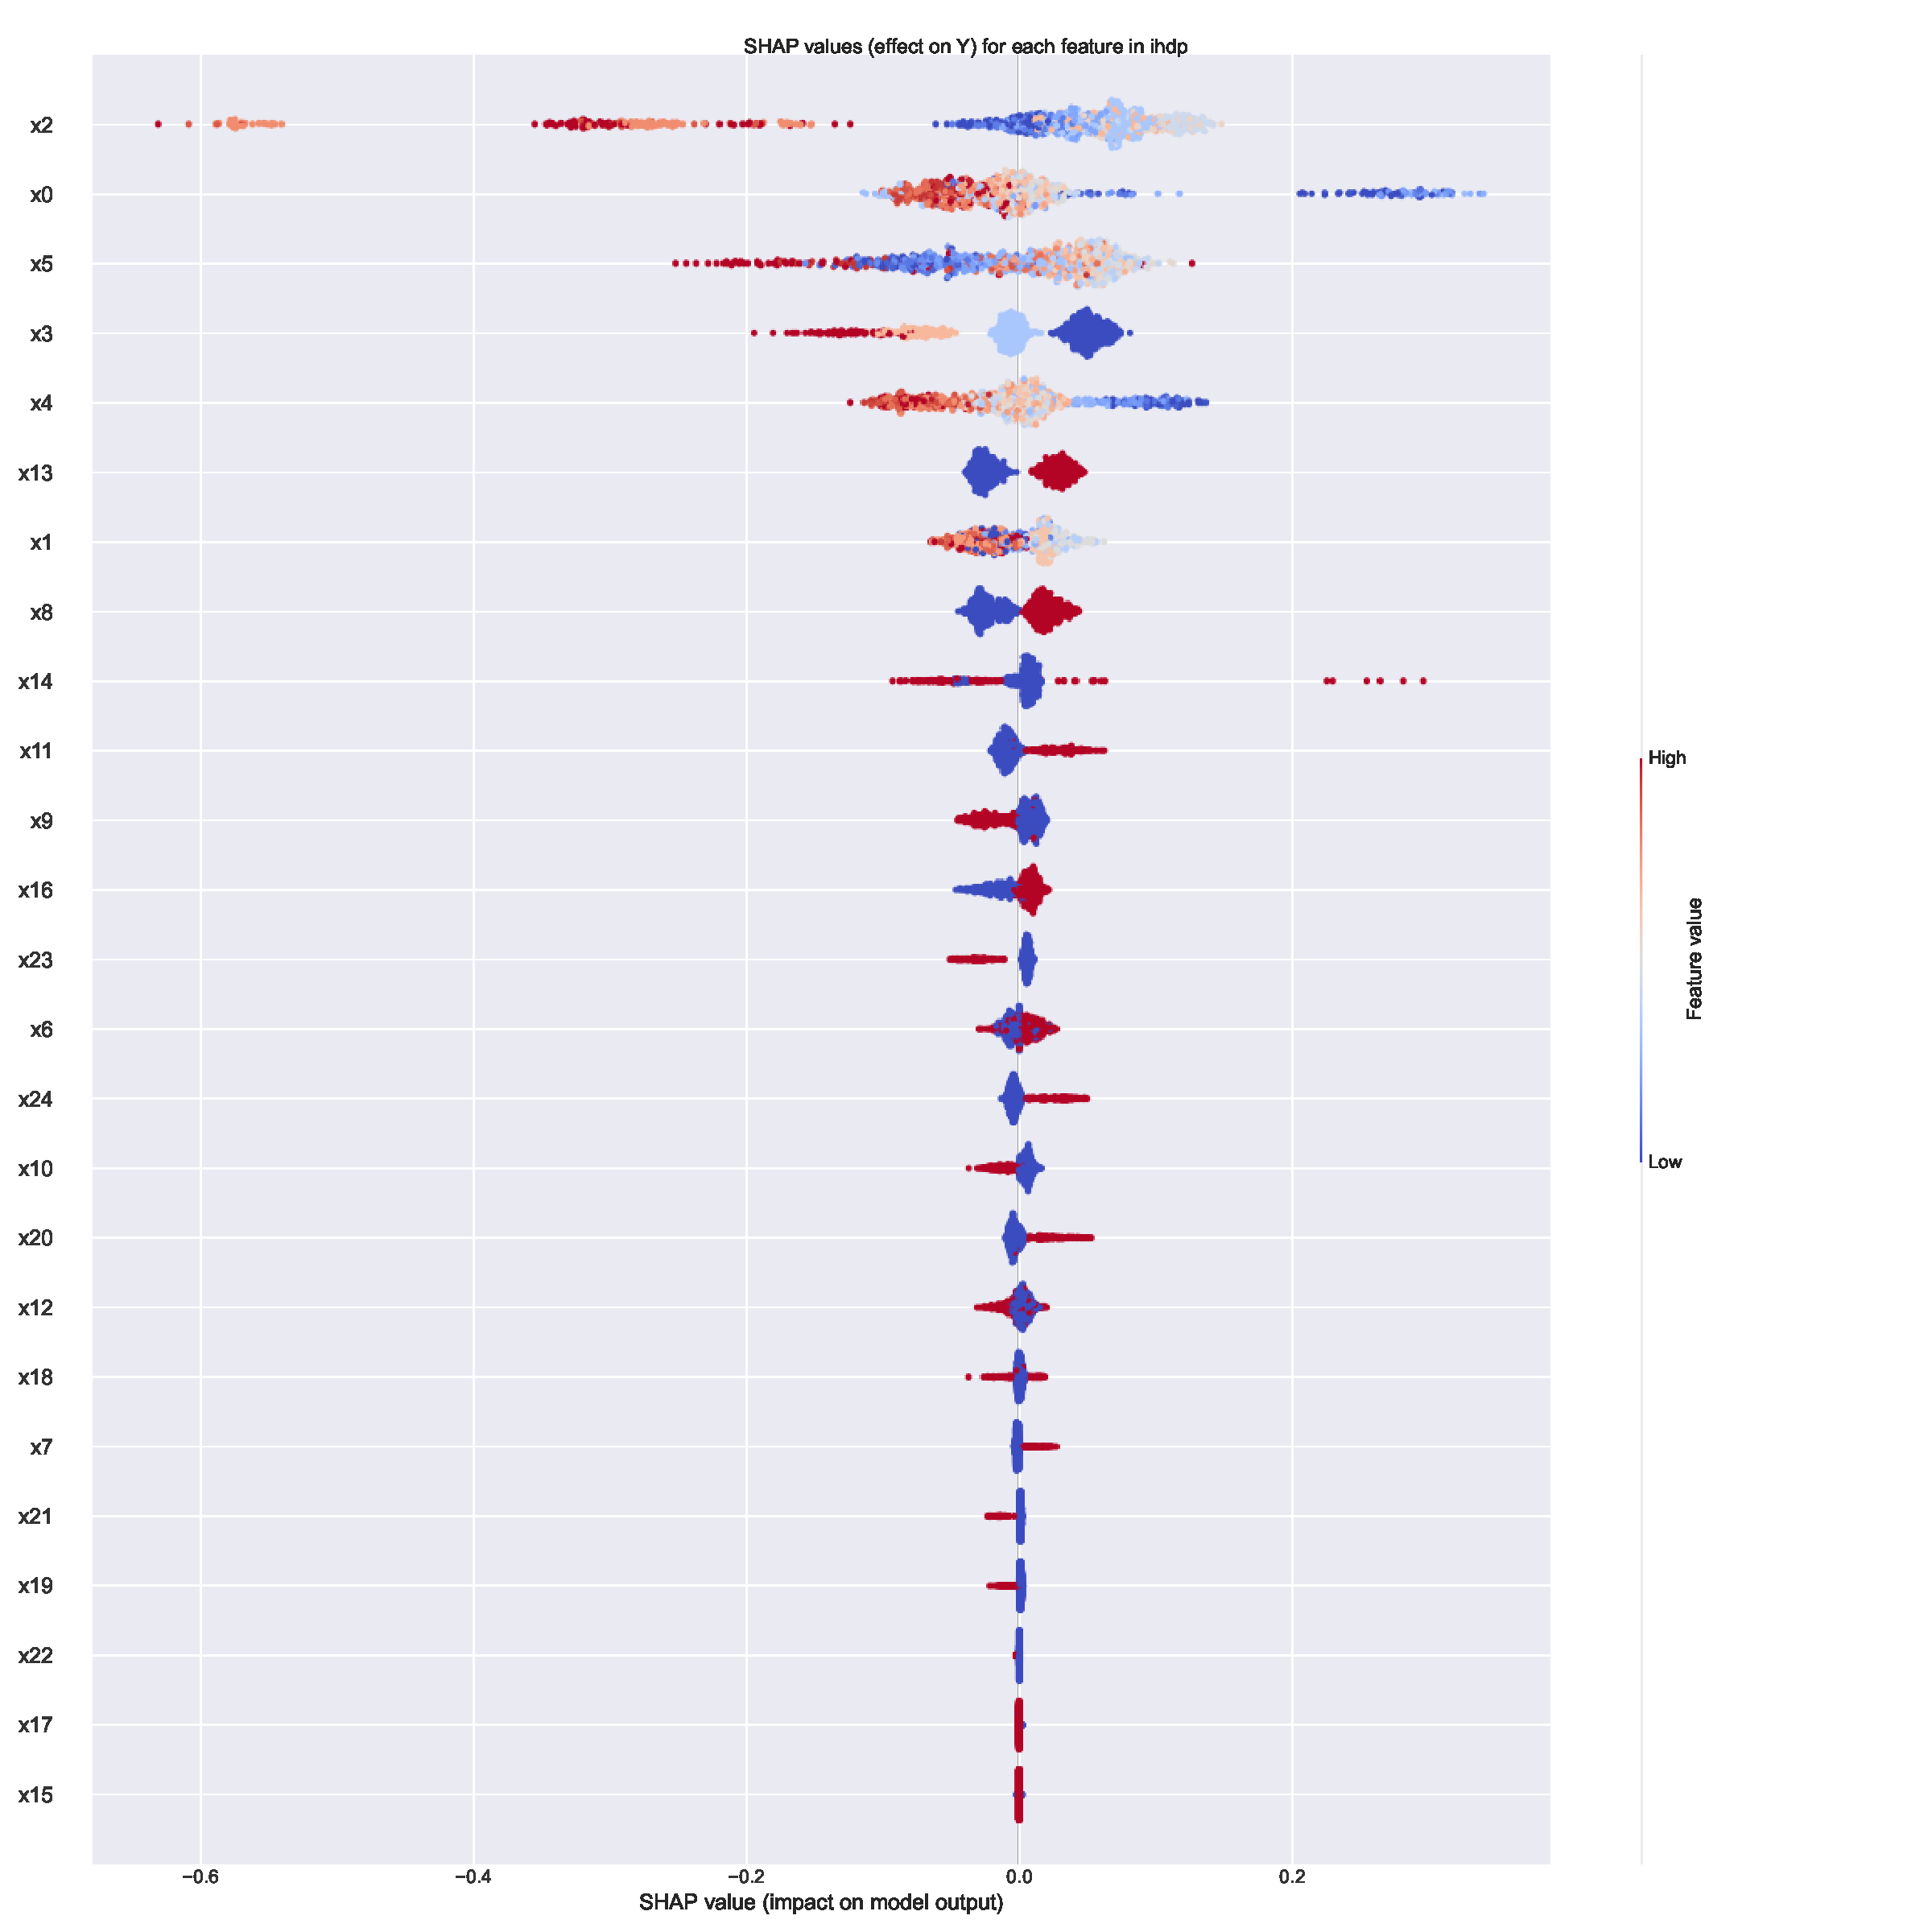
\includegraphics[width=1\linewidth]{project/assignment2/ihdp/ihdp SHAP values for Causal Forest.pdf}
\caption{Shapley values for the features in IHDP Causal Forest DML}
\label{fig:ihdpCATEcfA}
\justifying
\small
These shapley values are somewhat unexpected, considering the lack of any resemblance they have
to the shapley values for the earlier predictors, especially the sudden importance given to x2.
The impacts of x2 are also somewhat unusual. It appears that higher x2 values have a strong negative
effect on y, with very low x2 having a negligible positive effect, whilst x2 values in the middle appear
to have somewhat positive effects on y. This same pattern of effects can also be seen in x5 (median
values->slightly positive, extreme high/low->somewhat negative) and x1. 
\end{figure}

\begin{figure}[H]
\centering
\begin{subfigure}{1\textwidth}
  \centering
  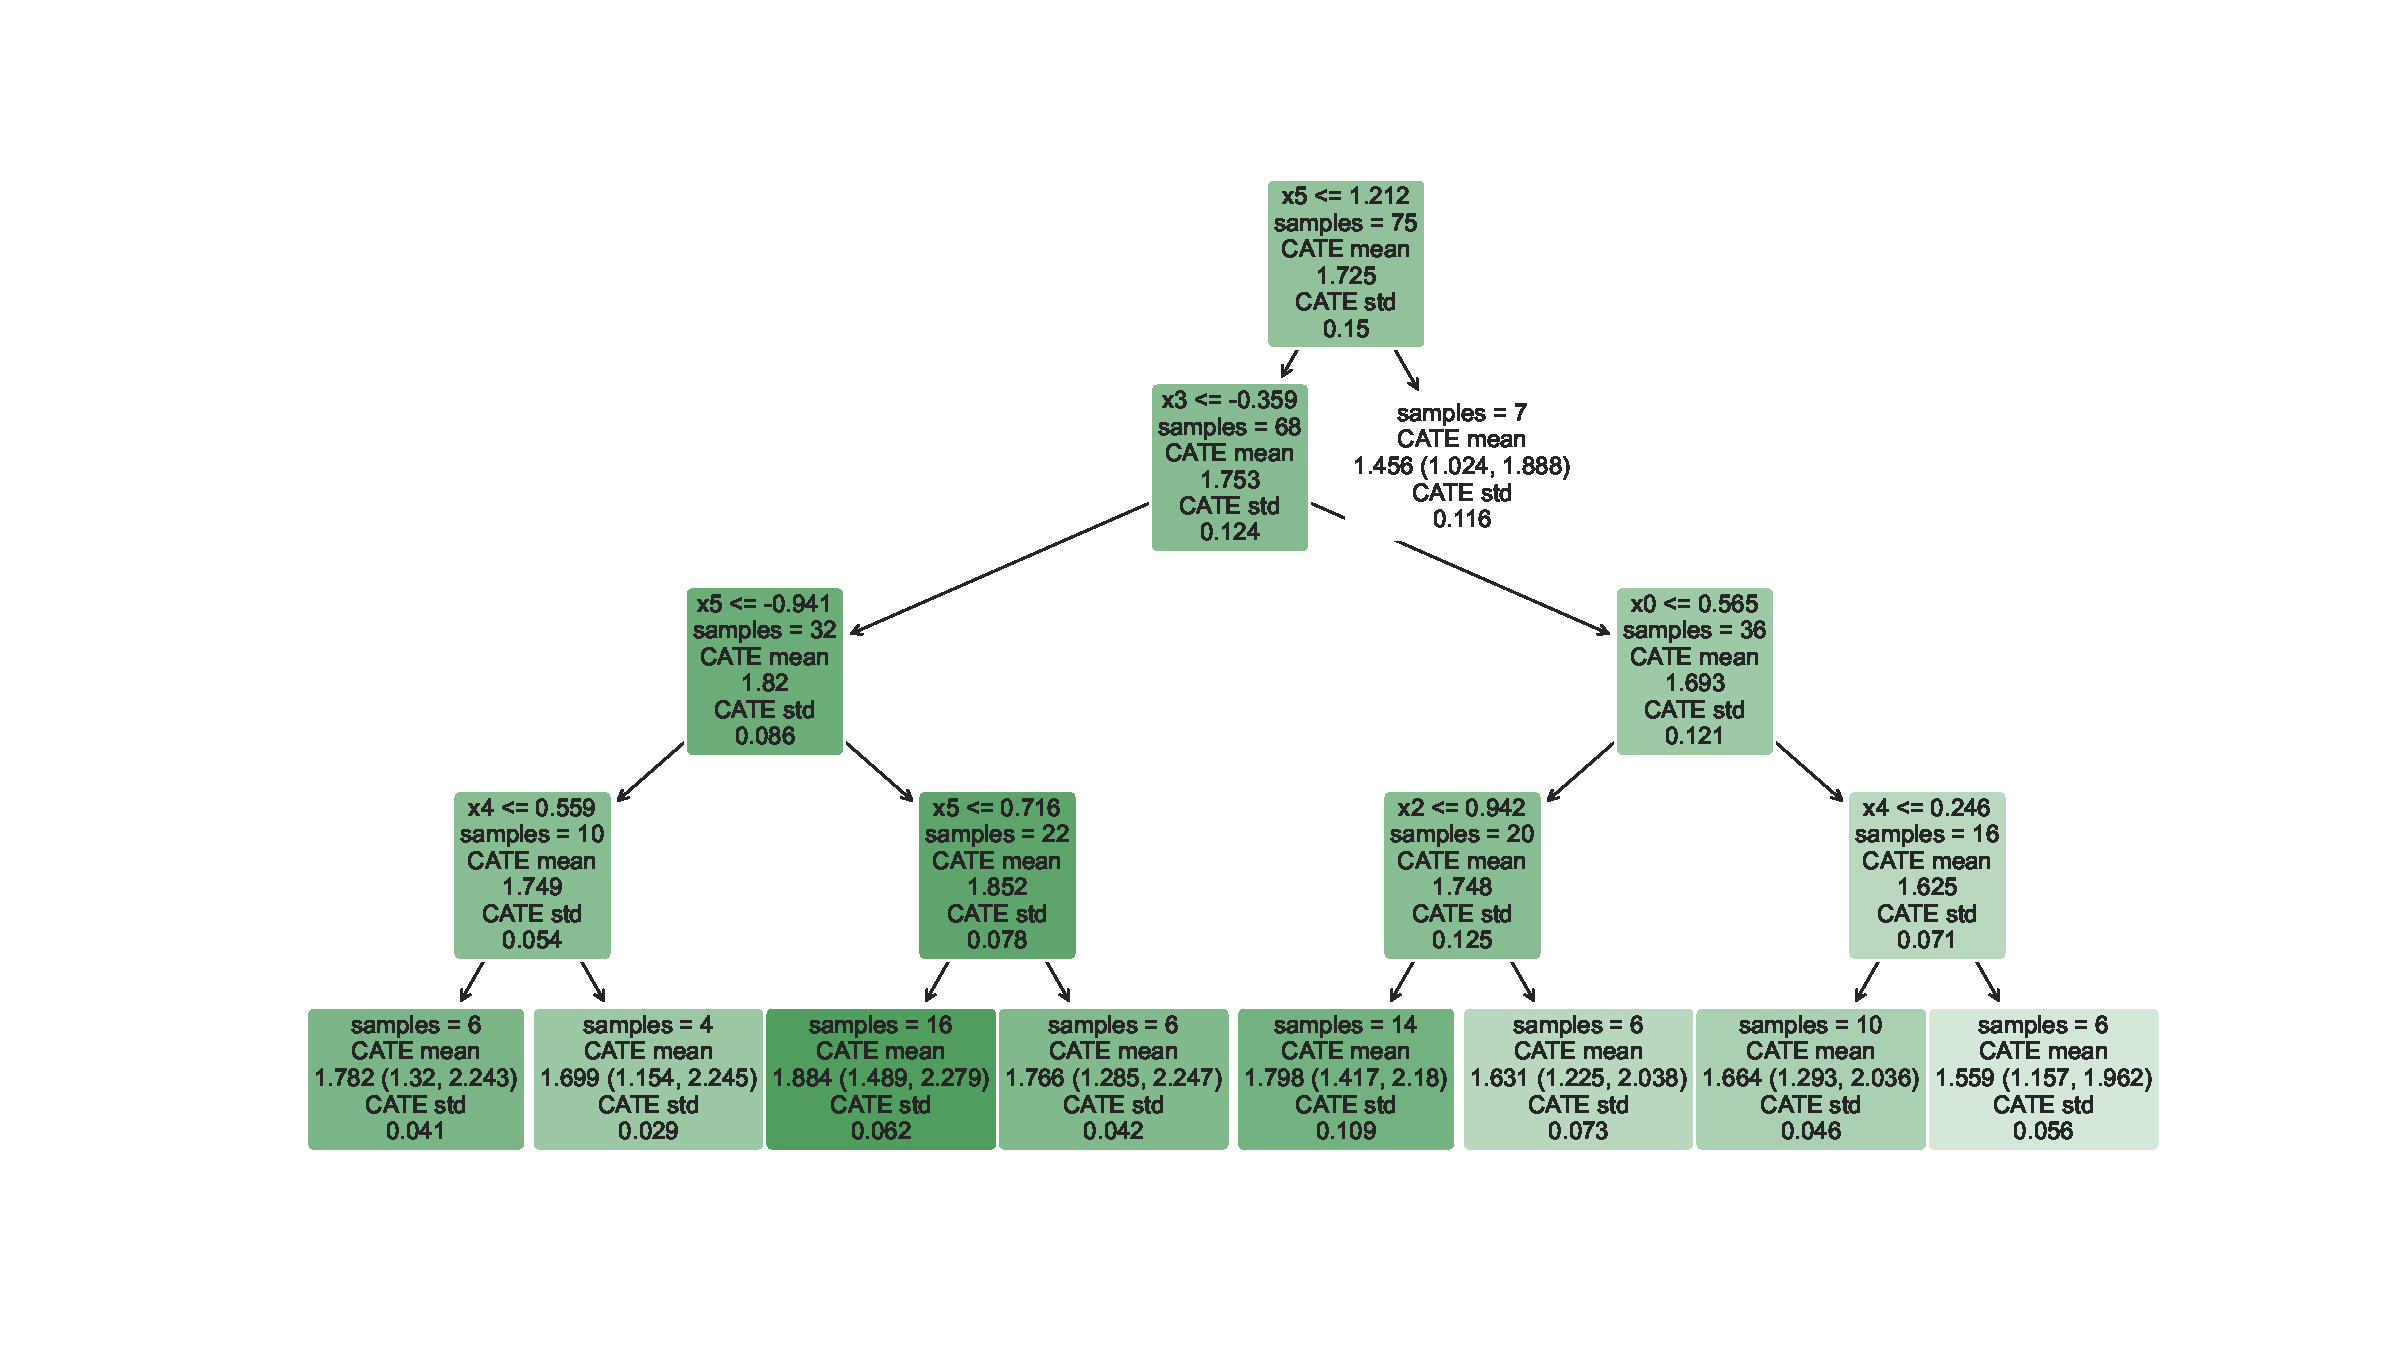
\includegraphics[width=1\linewidth]{project/assignment2/ihdp/Causal Forest CATE tree.pdf}
  \caption{CATE interpreter tree for IHDP Causal Forest DML}
  \label{fig:ihdpCATEcfB}
\end{subfigure}
\begin{subfigure}{1\textwidth}
  \centering
  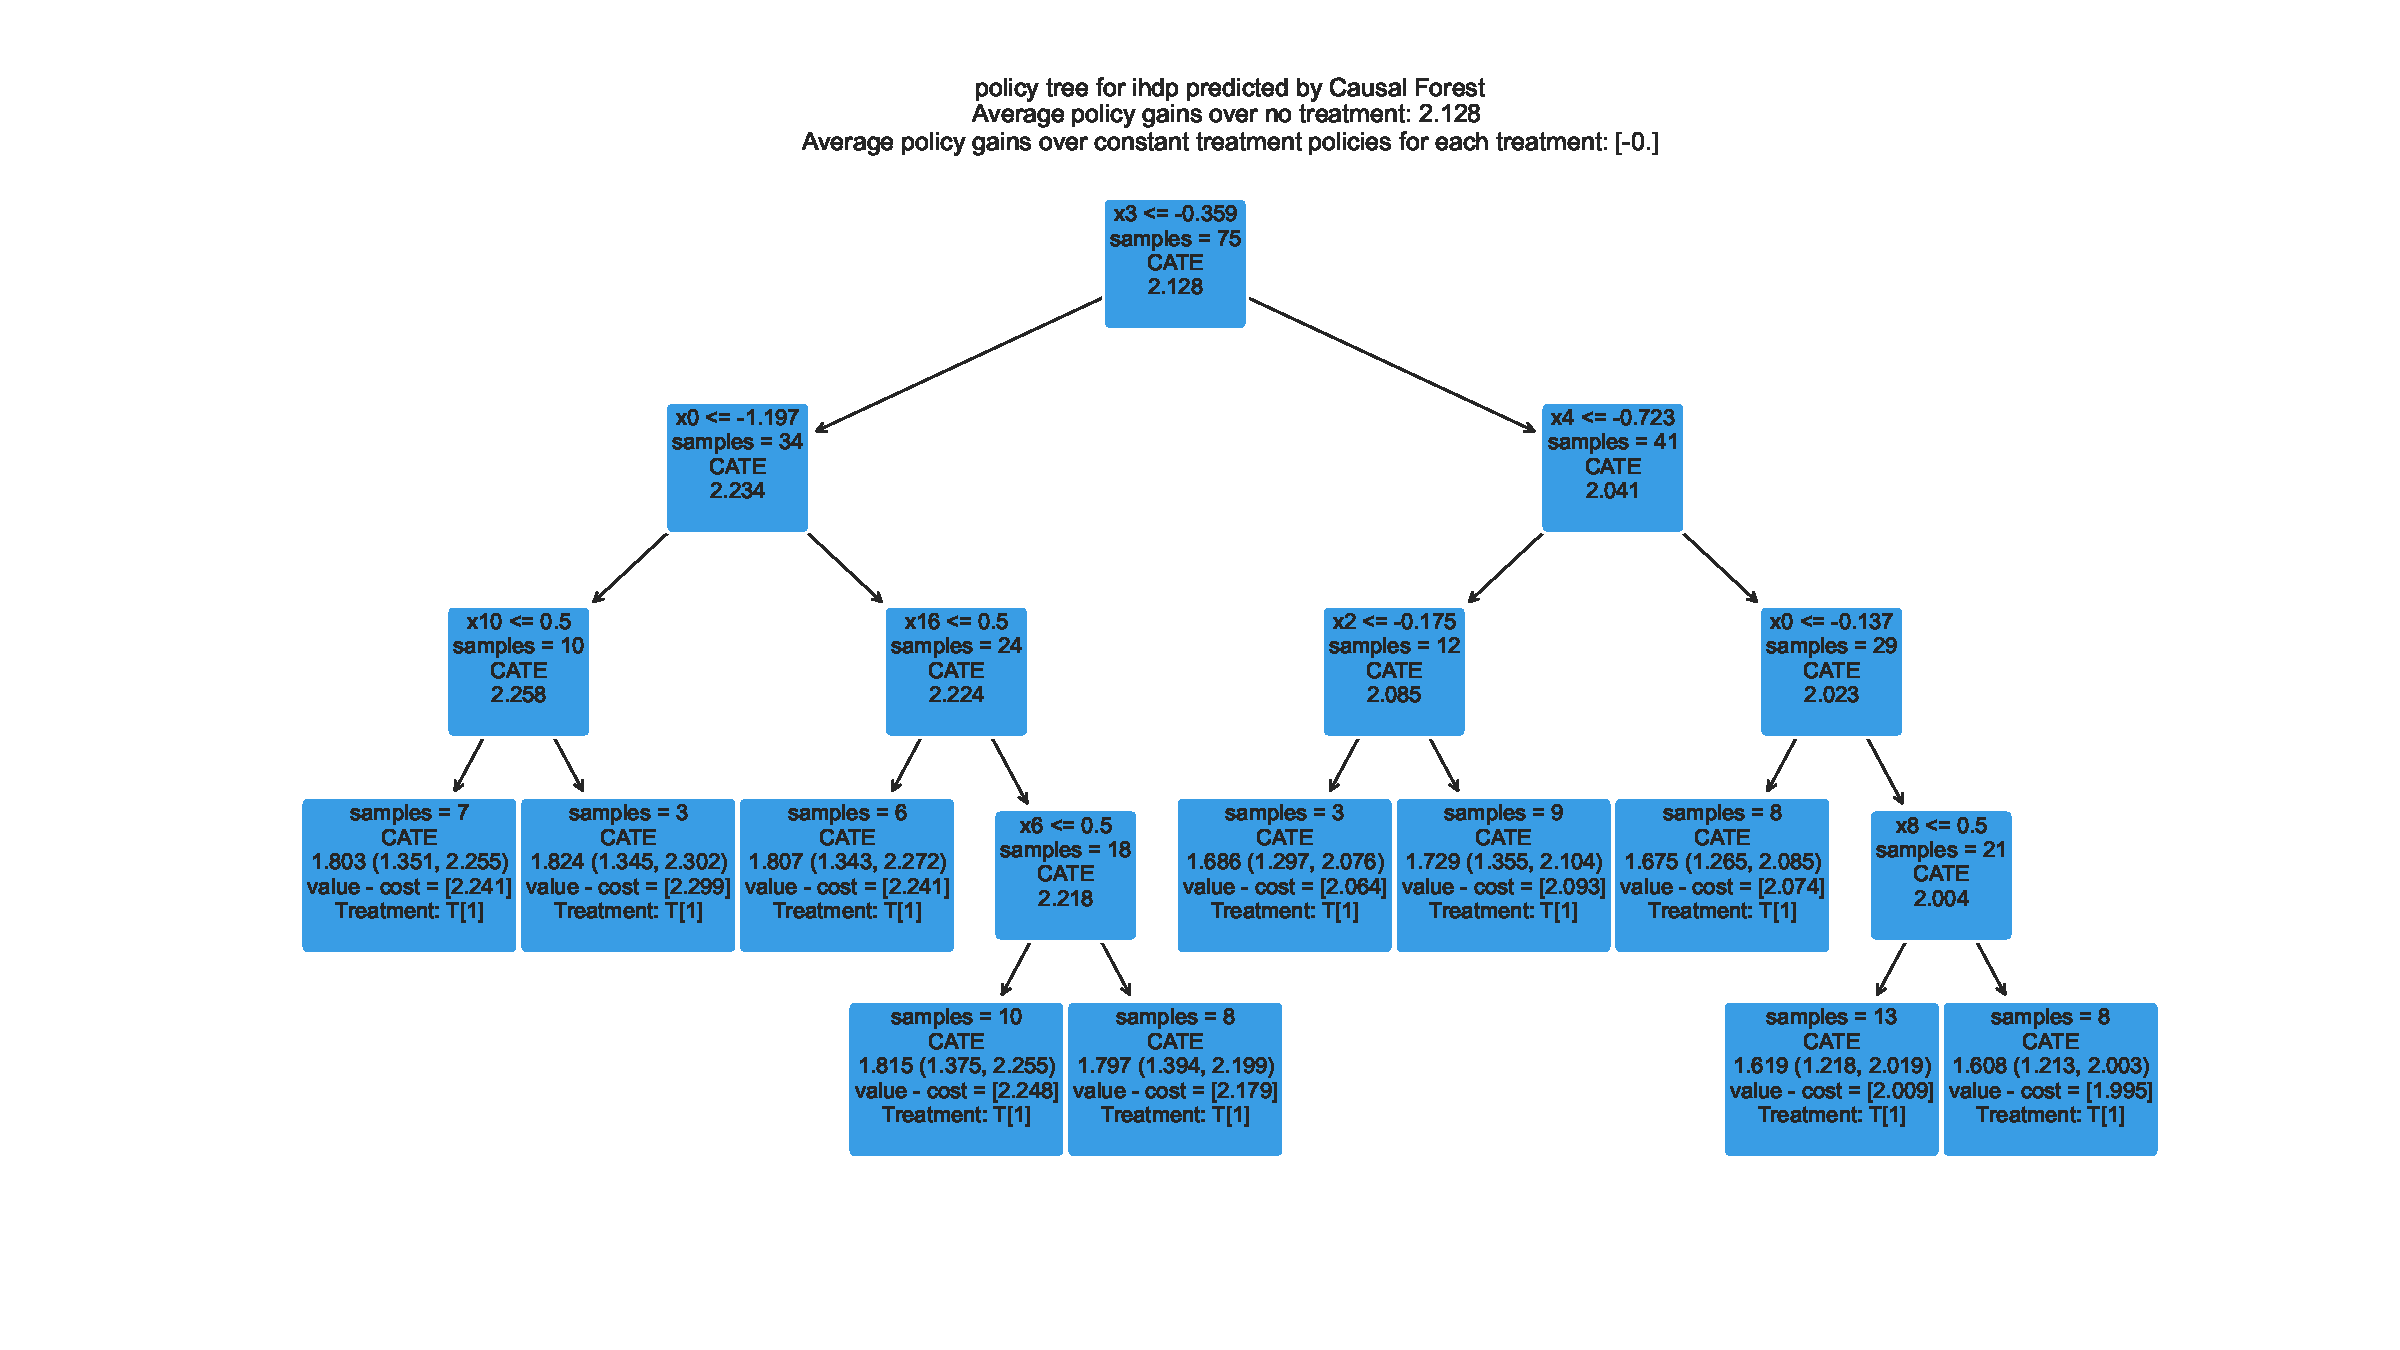
\includegraphics[width=1\linewidth]{project/assignment2/ihdp/Causal Forest policy tree.pdf}
  \caption{Policy interpreter tree for IHDP Causal Forest DML}
  \label{fig:ihdpCATEcfC}
\end{subfigure}
\caption{Interpreter trees for the IHDP Causal Forest DML}
\label{fig:ihdpCATEcf}
\justifying
\small
These trees are interpretations of the inner workings of the Causal Forest DML CATE estimator (with these
trees being constructed by \cite{shaptree}), and all give the impression of a rather optimistic outlook on
how the treatment effects the individuals involved. Granted, looking at the raw data for IHDP, there are
very few cases where an individual has a worse outcome for t=0 than t=1, so the policy illustrated in
\ref{fig:ihdpCATEcfC} to always treat (only with the extent of the treatment benefit fluctuating) does
make sense. This is also reflected in the CATE interpreter tree (\ref{fig:ihdpCATEcfB}), as, whilst there
are a few outlier cases in the full dataset where the effect is negative, none of those samples are in
the test set, therefore, once again, it's just the scale of the benefit that fluctuates.
\end{figure}

\FloatBarrier


\subsection{JOBS}

\subsubsection{Simple Learners (Y given XT)}

\FloatBarrier

The learner with the best `ROC AUC` score was the `SGDClassifier`, with an `ROC AUC` score on the test
set of 0.76. As can be seen from Figure \ref{fig:jobsSimple}, the features with the strongest
impact on the outcome appear to be `x6` and `x11`, then `x7` and `x12`, whilst `t` has a negligible
importance.

The lack of any influence from `t` is somewhat unexpected.

\begin{figure}[H]
\centering
\begin{subfigure}{.5\textwidth}
  \centering
  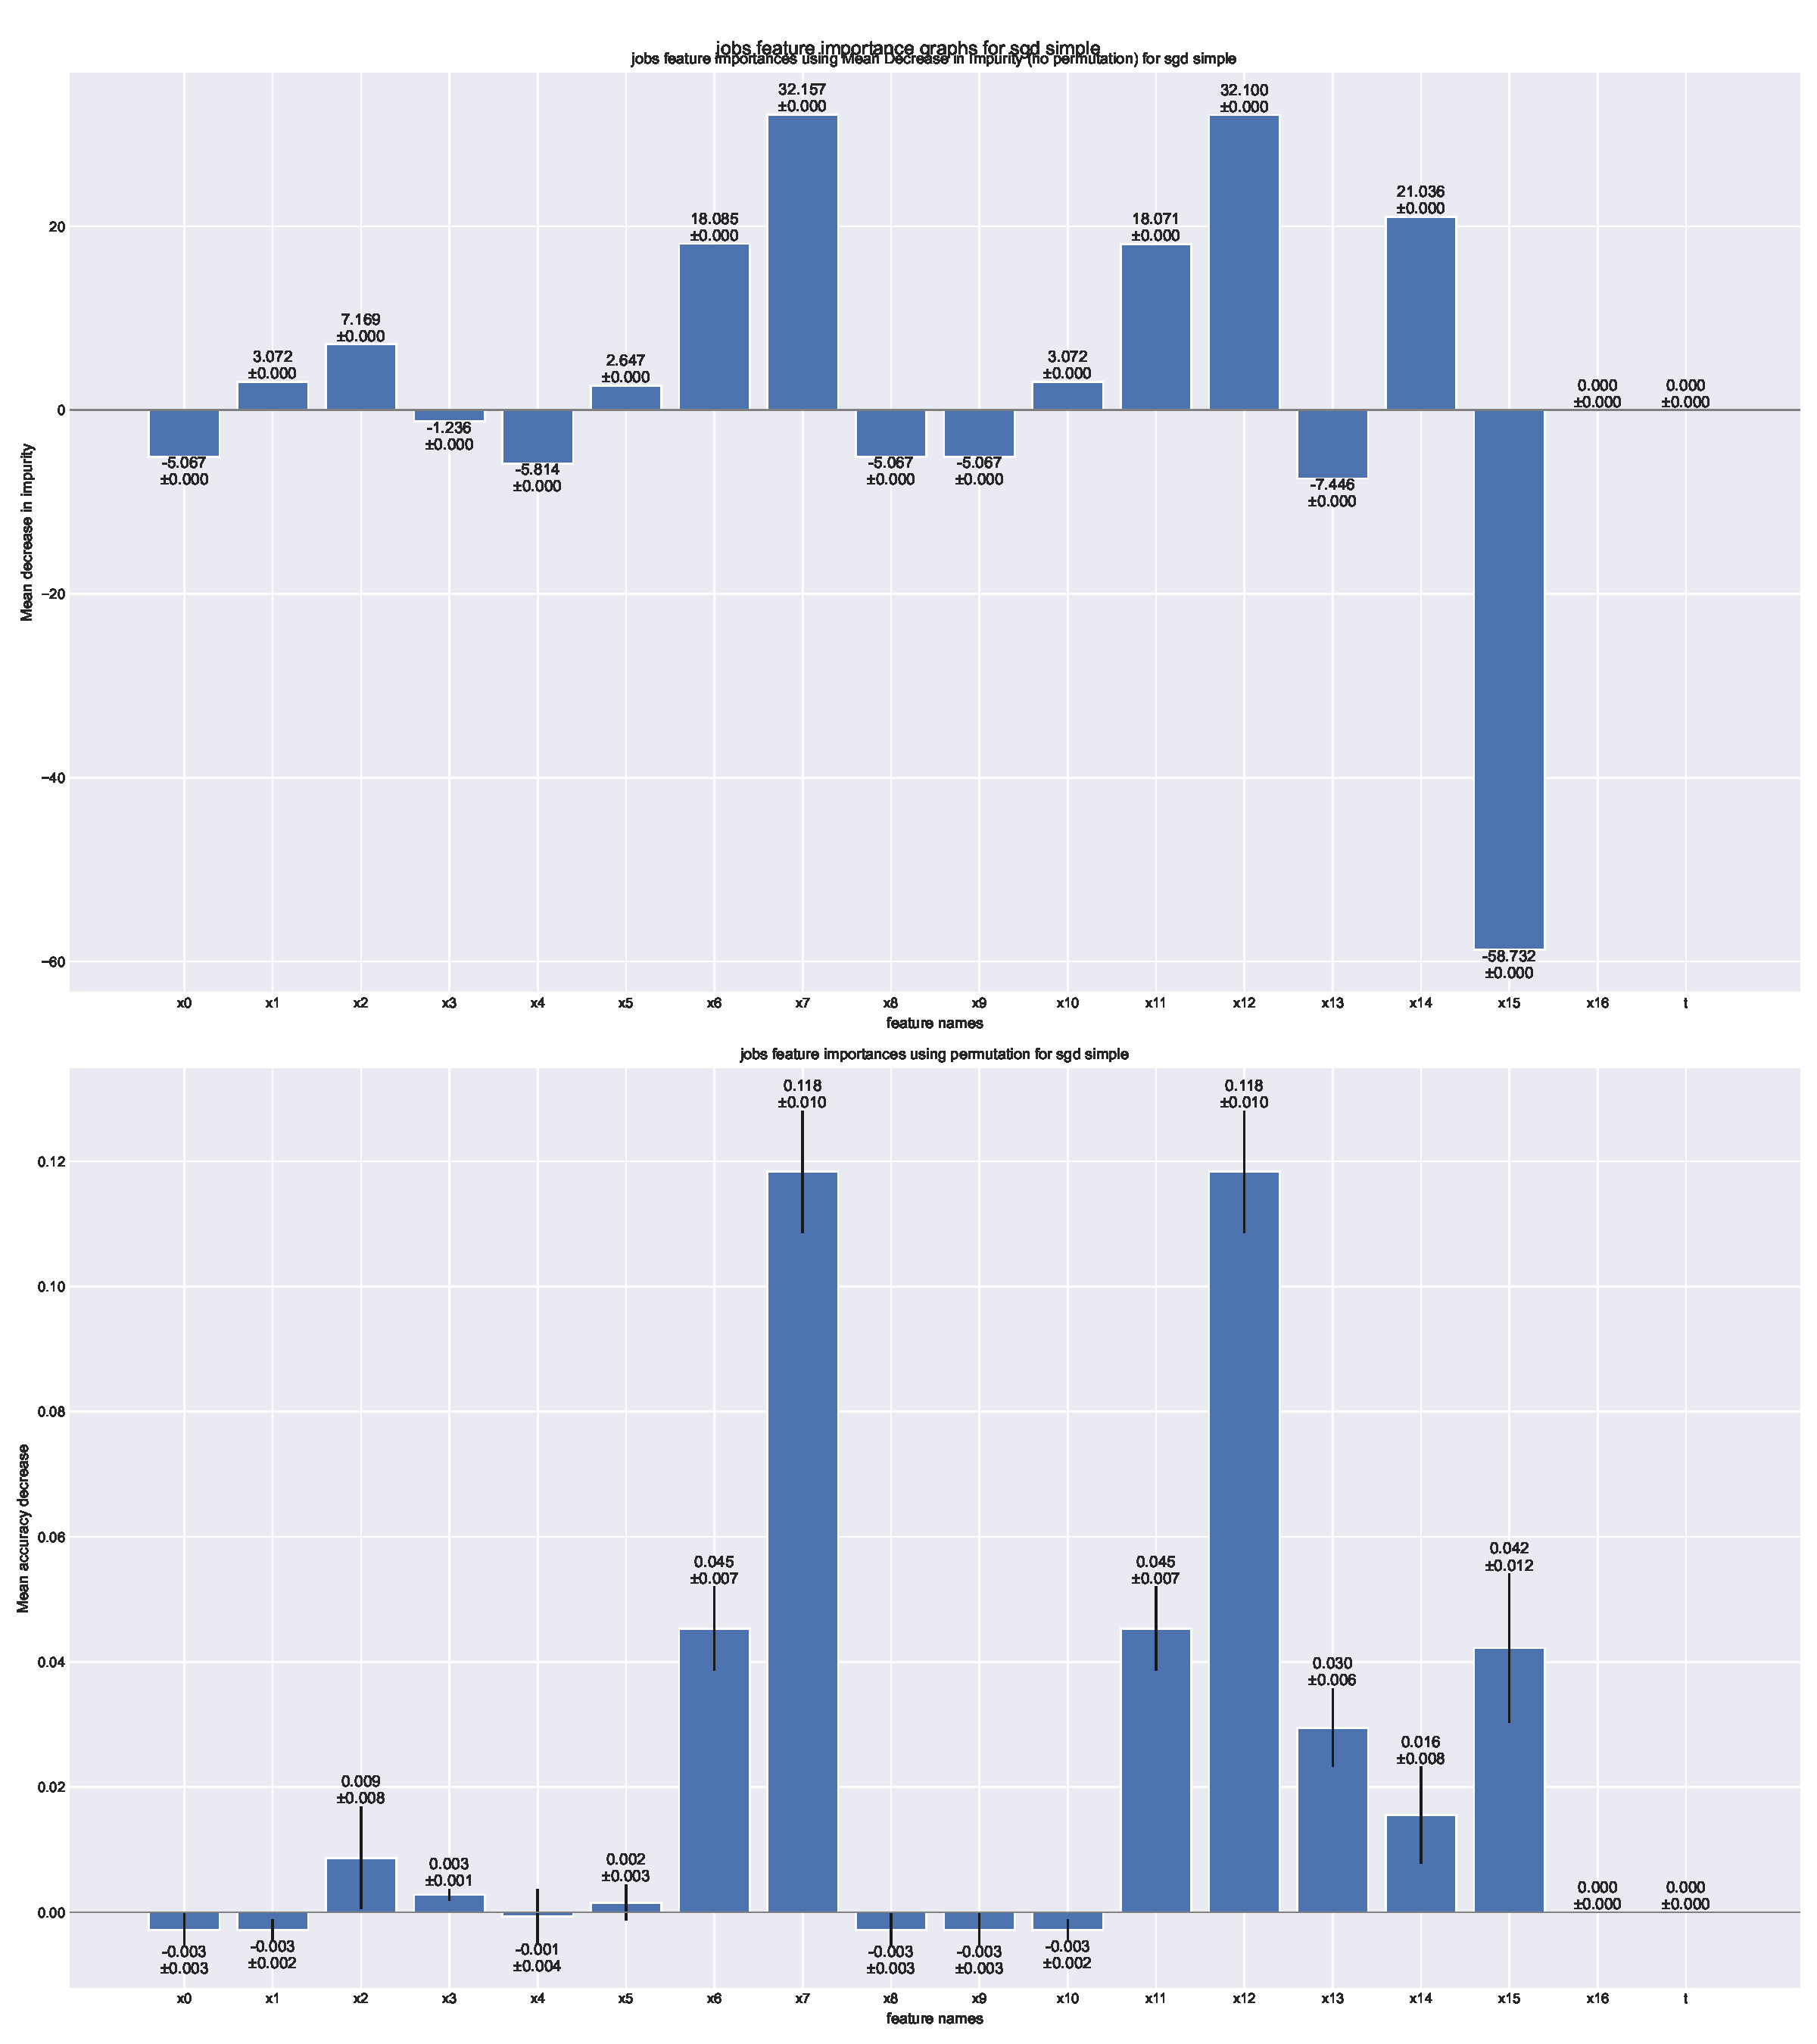
\includegraphics[width=1\linewidth]{project/assignment2/jobs/jobs sgd simple feature importances.pdf} 
  \caption{Feature importances (from coeff\_ and permutation\_test) for JOBS simple SGDClassifier}
  \label{fig:jobsSimpleA}
\end{subfigure}%
\begin{subfigure}{.5\textwidth}
  \centering
  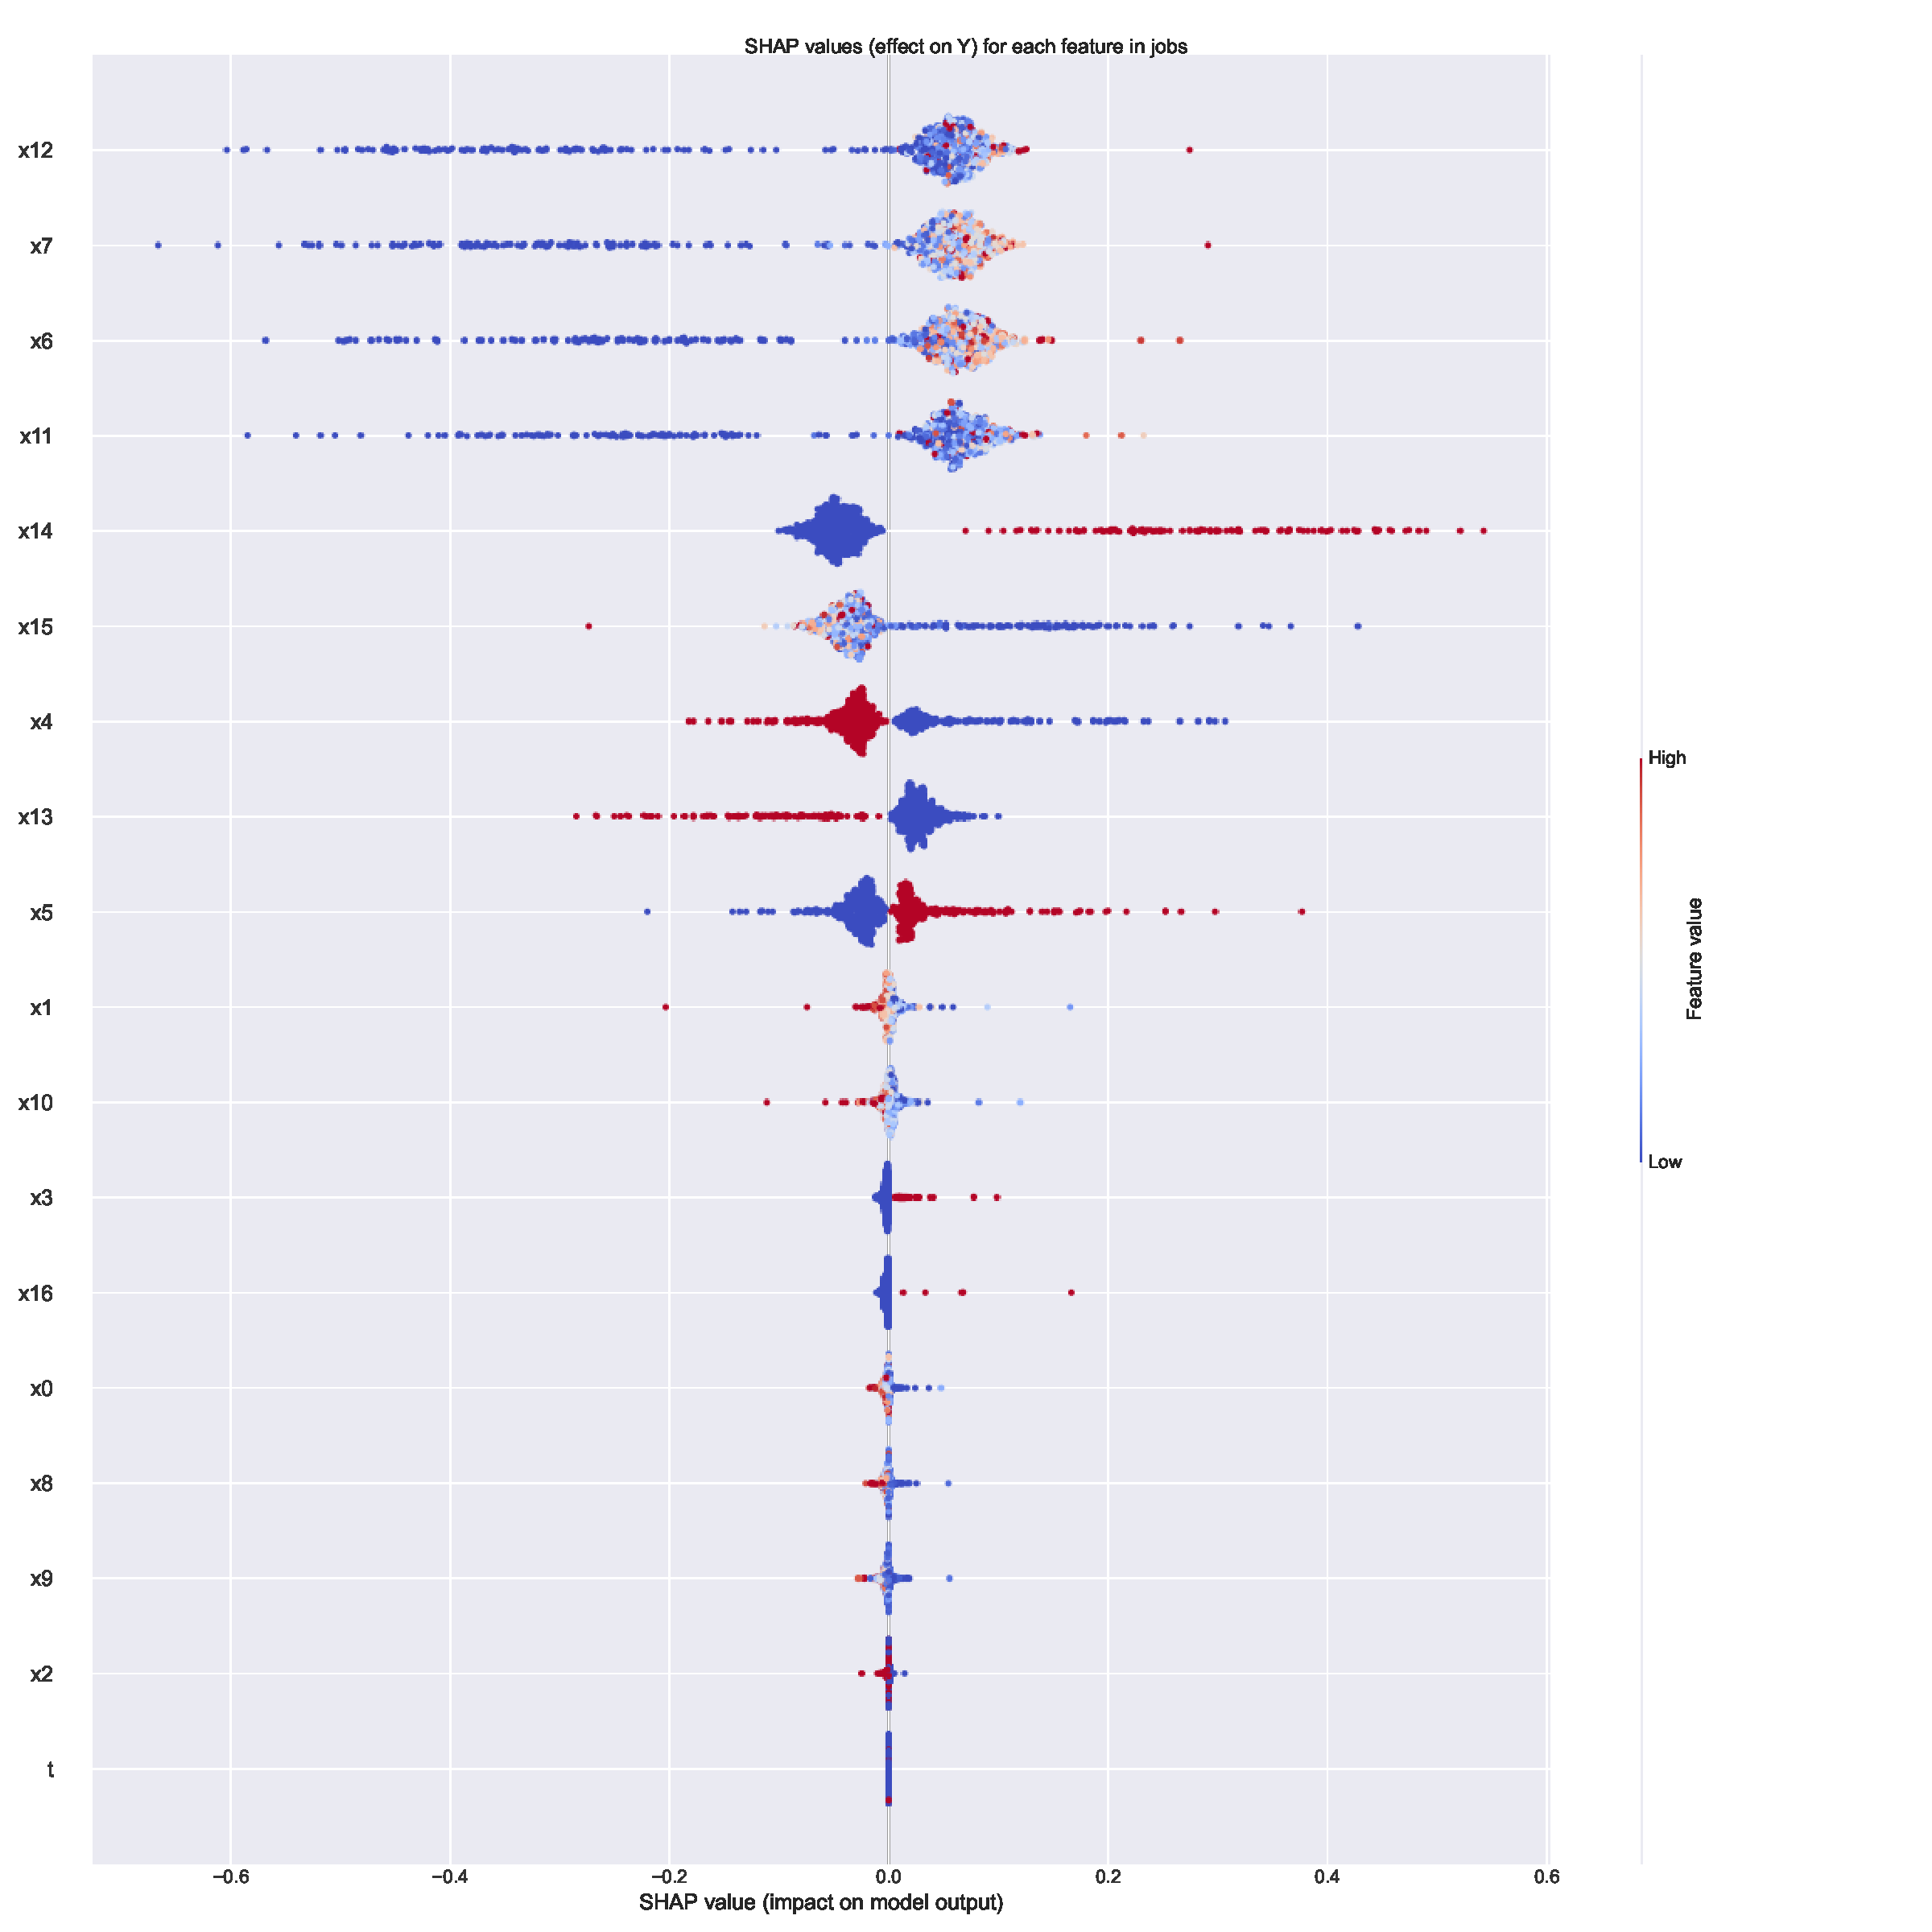
\includegraphics[width=1\linewidth]{project/assignment2/jobs/jobs SHAP values for sgd simple.pdf}
  \caption{Shapley values for the features as found by the JOBS Y|XT SGDClassifier}
  \label{fig:jobsSimpleB}
\end{subfigure}
\caption{Feature importances found by the Jobs Y|XT learner}
\label{fig:jobsSimple}
\small
\justifying
Looking at Figures \ref{fig:jobsSimpleA} and \ref{fig:jobsSimpleB}, `t` appears have no impact on the `y`
outcome for an individual, indicating that the treatment may not be having any impact at all. However,
if we remember that JOBS is a combination of experimental and observational data, and that the relative
size of the treatment group is particularly small (leading to the vast majority of the data being about
untreated individuals), it's understandable how `t`, being only applicable to a minority,
would not be seen as having any bearing on the outcome for the majority.

That said, it is interesting how, in \ref{fig:jobsSimpleB}, the four 'most important' features, `x6`,
`x7`, `x11`, and `x12` all have a shape in this graph somewhat reminiscent of a pike (or some other big
stick with a big pointy bit at the end), specifically with how higher values lead to a higher `y`, then
the most common 'lower' values also have a (lesser) positive `y` effect, with the `y` effect generally
getting worse as these features degrade further. Features `x14` and `x15` have somewhat similar shapes,
but reversed (`x14`: the lower values are the 'spike' and are negative, higher is the 'stick' and is
positive; `x15`: literally just the reverse of `x6`,`x7`,`x11`,and `x12`).
These similar distributions imply that there may be a causal link between these features.
\end{figure}

\FloatBarrier

\subsubsection{IPSW learners (T given X)}

\FloatBarrier

The best estimator for `T|X` for `JOBS` was also the SGD classifier, with a
`ROC AUC`\footnote{Receiver Operator Characteristic Area Under Curve} score of 0.62 on the test set.
The feature importances of this classifier (Figure \ref{fig:jobsIPSW}) appear to be completely different 
to the IHDP `Y|XT` classifier,
with `x5` and `x14` having rather low importances, whilst several other features all compete to have
the highest importance, with wildly fluctuating standard deviations for the importance predictions
visible in Subfigure \ref{fig:jobsIPSWA}. 

The shapley values (Subfigure \ref{fig:jobsIPSWB}) are somewhat more coherent;
for all of the binary features, values of `0` and `1` have
opposing impacts on the final `t` value\footnote{By this, I mean that 'for the ones where xN=0 has a negative effect, xN=1 has a positive effect, and vice versa'}. The continuous values are a bit more
fuzzy in this regard, but they mostly follow this rule of 'bigger has opposite sign effect to smaller'.
The only real exception is with `x3`; the high and slightly low values of `x3` have negative impacts,
and only the particularly small `x3` values have a positive impact.

The rather extreme effects of `x5` and `x4` on `t`, combined with the consistent direction of the impacts,
indicates that `x5` and `x4` could potentially be related to an individual's eligibility to have been
included in the treatment group (whether or not that it would have lead to the individual being treated
is somewhat questionable). However, it's also possible that the other features where the high/low values
for that feature were all present on the same side as each other could have been related to eligibility.

\begin{figure}[H]
\centering
\begin{subfigure}{.5\textwidth}
  \centering
  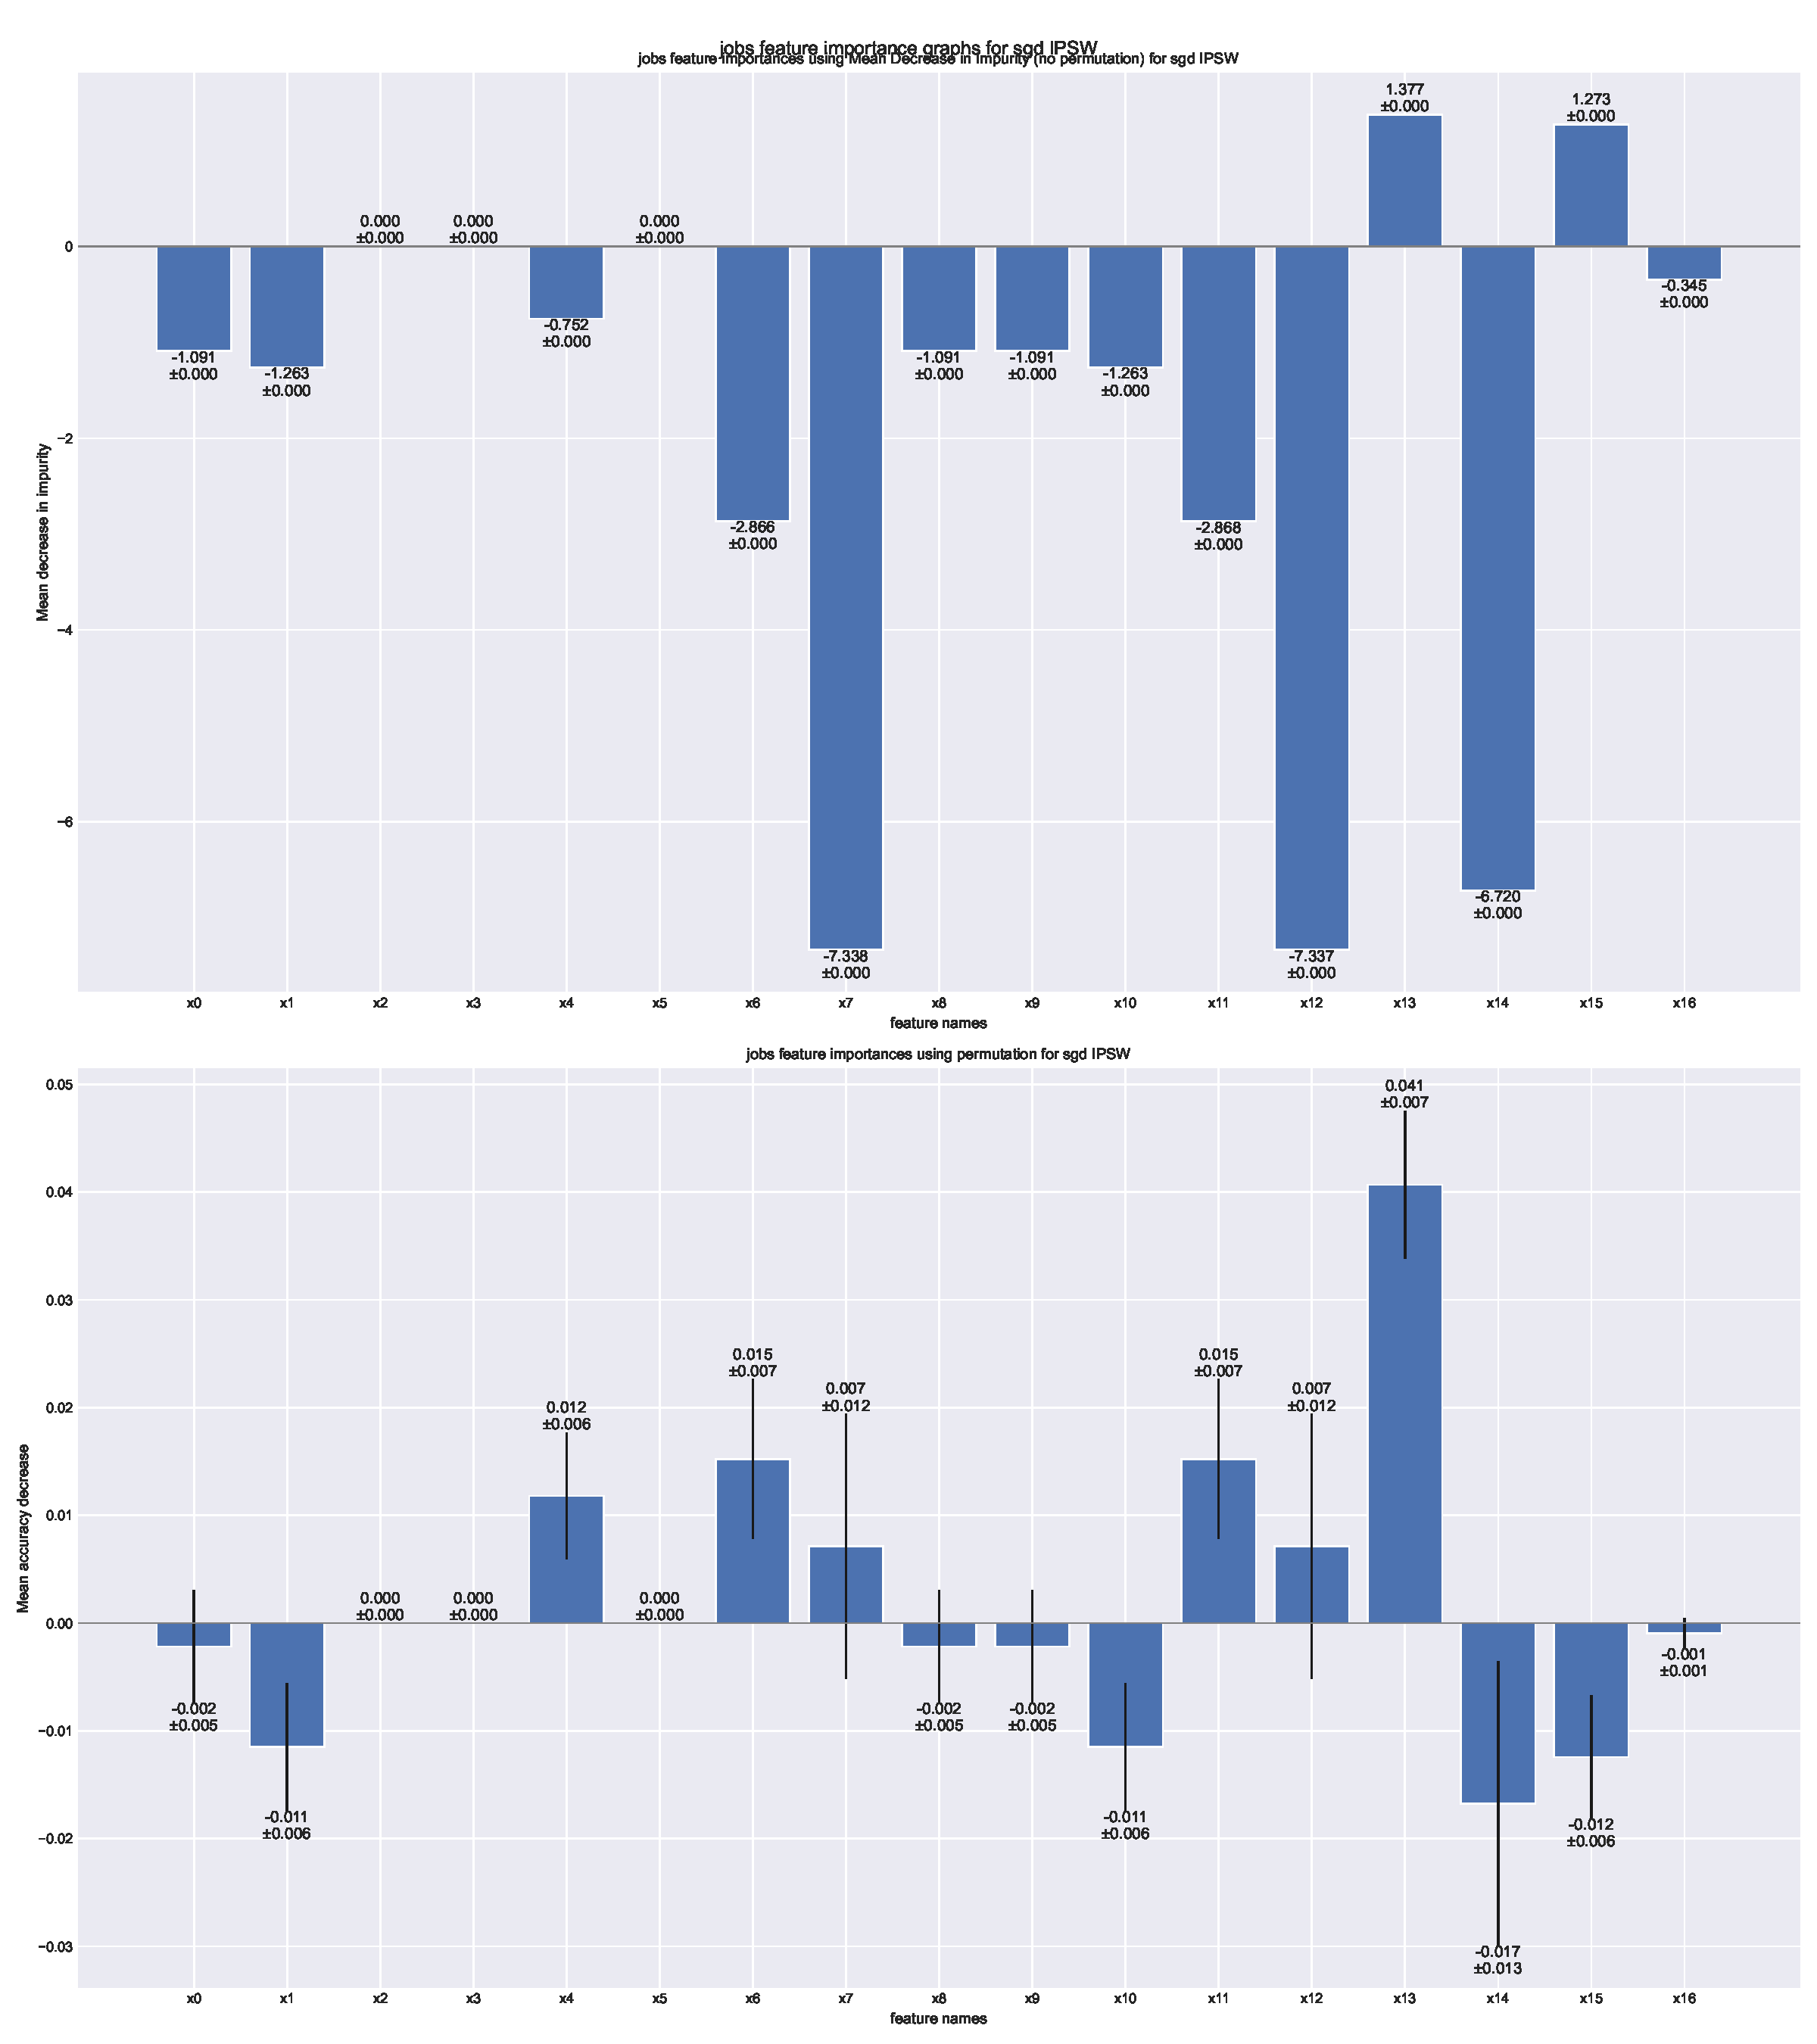
\includegraphics[width=1\linewidth]{project/assignment2/jobs/jobs sgd IPSW feature importances.pdf}
  \caption{Feature importances (from feature\_importances\_ and permutation\_test) for JOBS IPSW SGD}
  \label{fig:jobsIPSWA}
\end{subfigure}%
\begin{subfigure}{.5\textwidth}
  \centering
  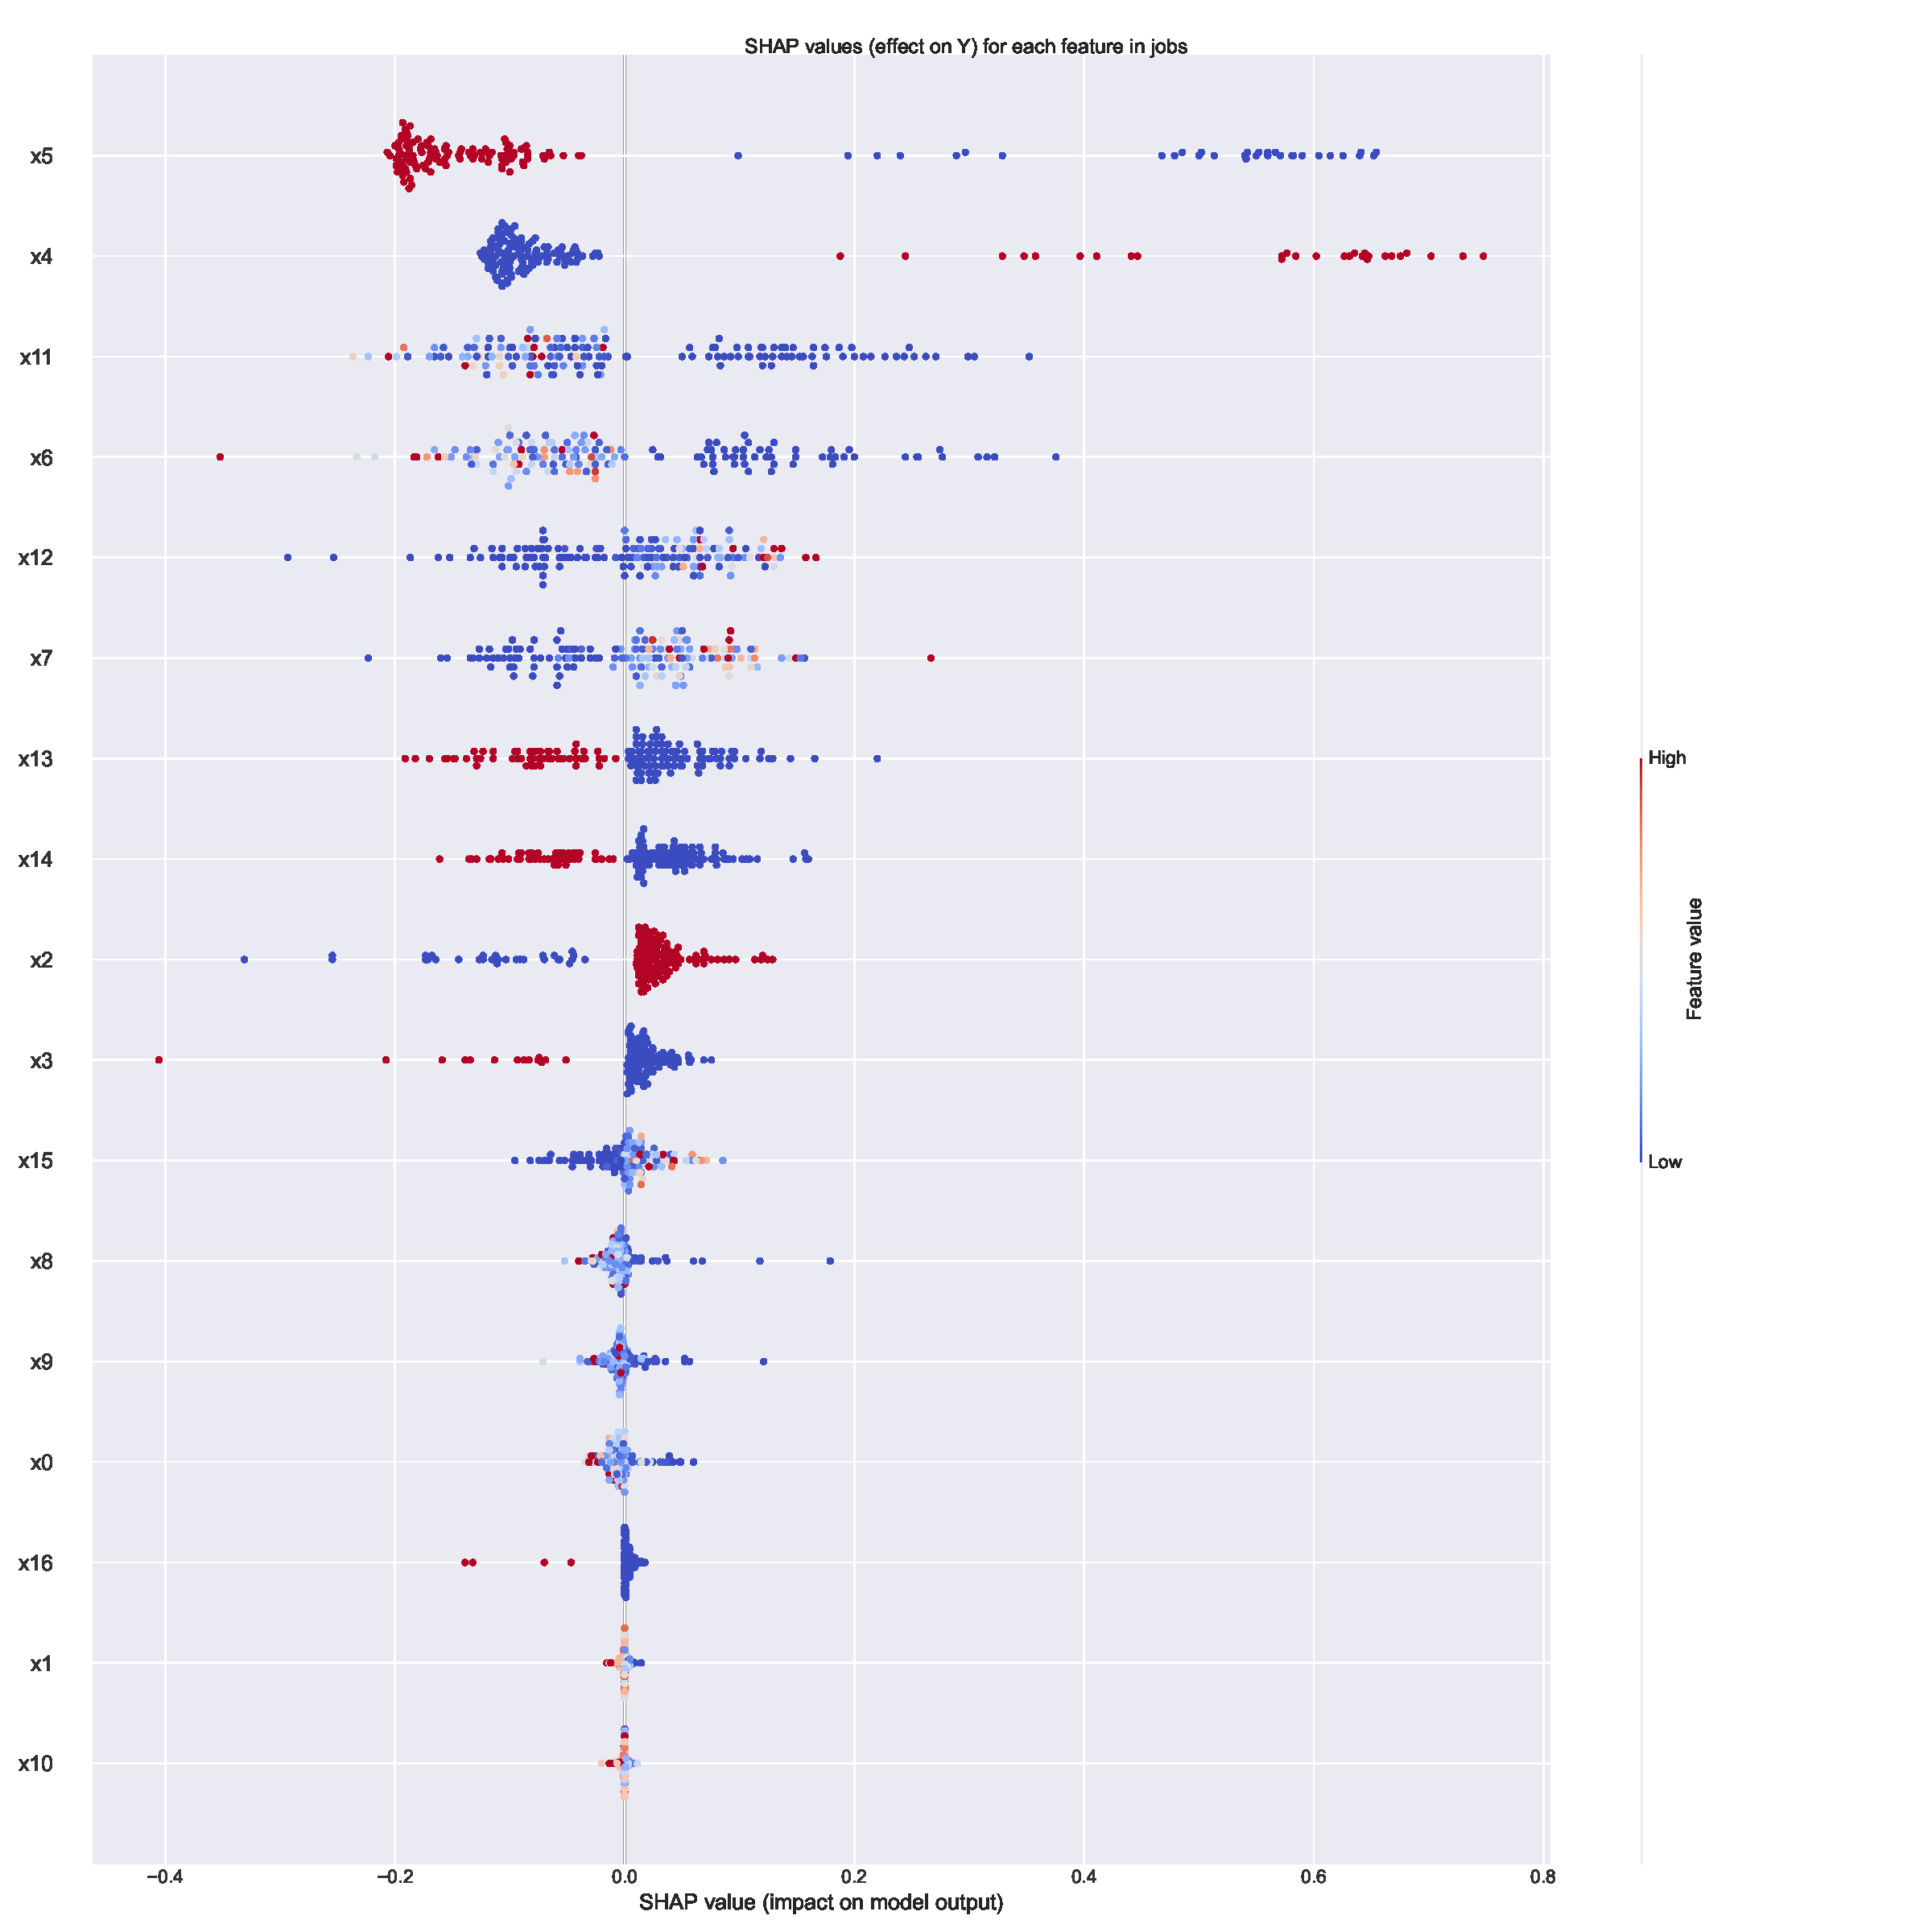
\includegraphics[width=1\linewidth]{project/assignment2/jobs/jobs SHAP values for sgd IPSW.pdf}
  \caption{Shapley values for the features as found by the IHDP T|X SGD predictor}
  \label{fig:jobsIPSWB}
\end{subfigure}
\caption{Feature importances found by the JOBS T|X learner}
\label{fig:jobsIPSW}
\end{figure}

\FloatBarrier


\subsubsection{JOBS simple learners with IPSW (Y given XT*IPSW(X))}

\FloatBarrier

Once again, the `SGDClassifier` had the best result (`roc\_auc` score of 0.76), and, once again,
as shown in Figure \ref{fig:jobsSimpleIPSW}, `x6`, `x7` ,`x11`, and `x12` have once again been
identified as the most important features, with `t` still being classed as unimportant (despite the
IPSW scores being used to apply sample weights during the training process), presumably due to the same
issues regarding the lack of samples with `t=1` for `t` to be considered to have had an impact.


\begin{figure}[H]
\centering
\begin{subfigure}{.5\textwidth}
  \centering
  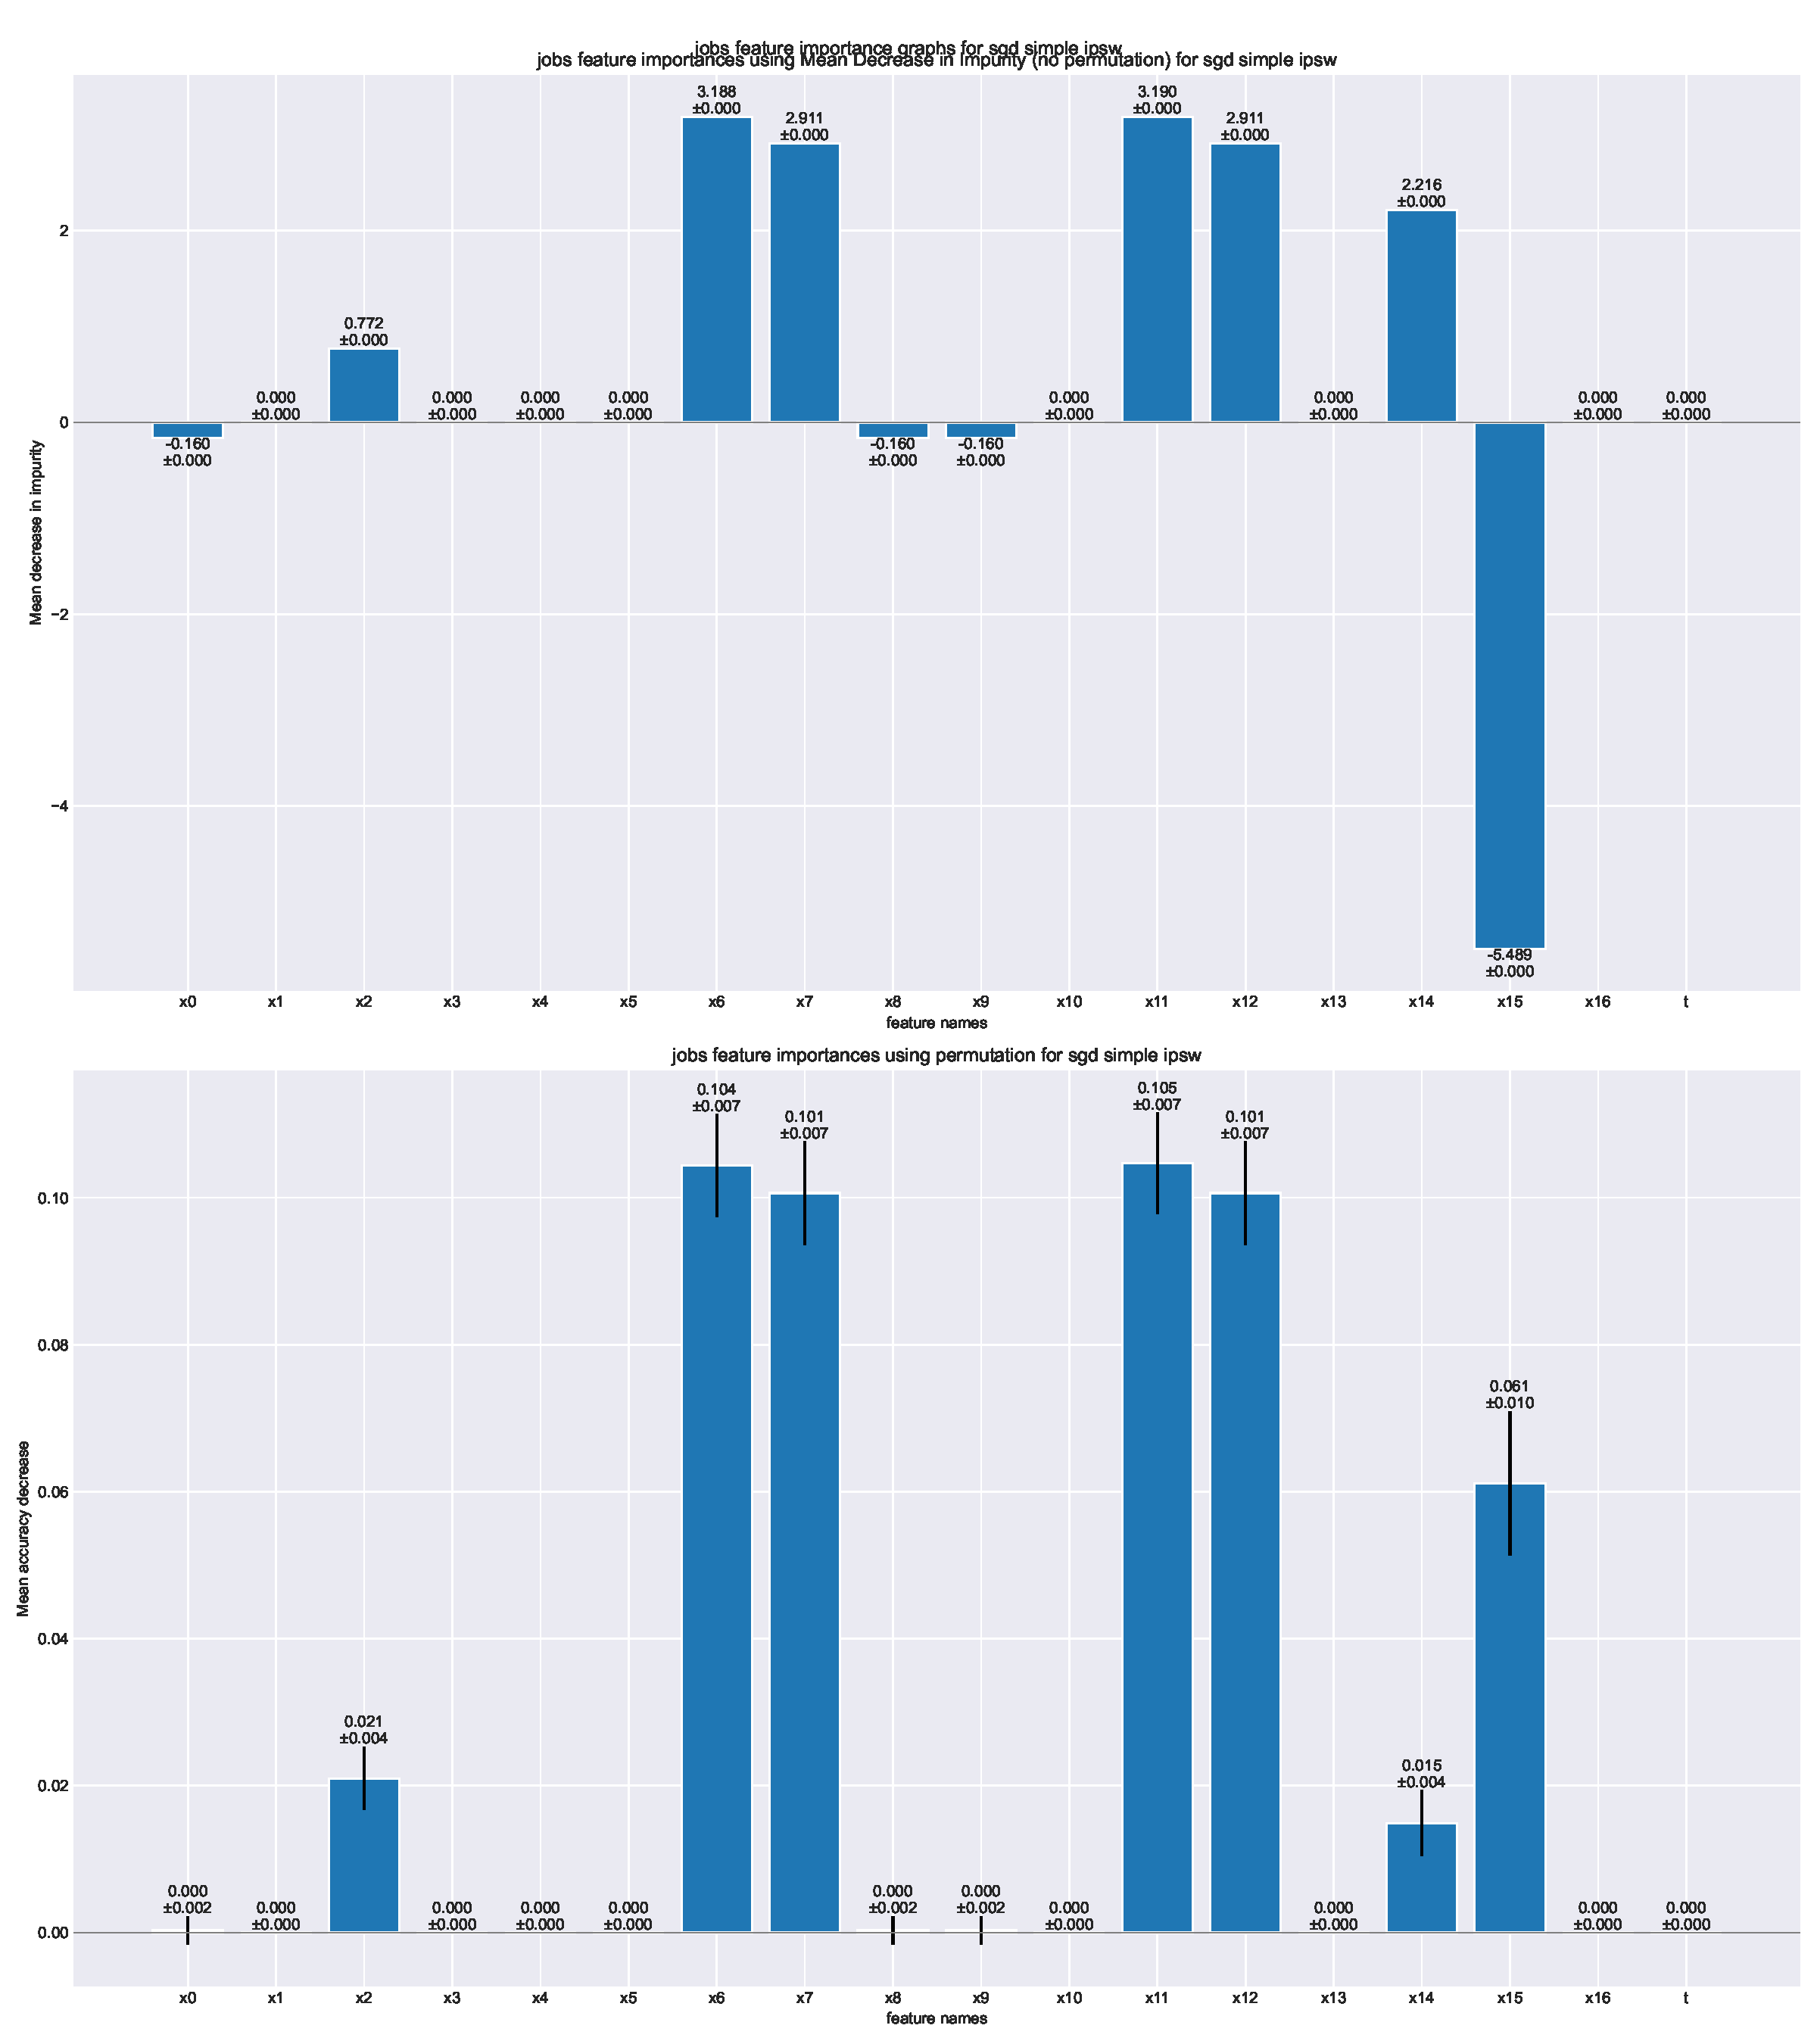
\includegraphics[width=1\linewidth]{project/assignment2/jobs/jobs sgd simple ipsw feature importances.pdf}
  \caption{Feature importances (from feature\_importances\_ and permutation\_test) for JOBS simple+IPSW SGD}
  \label{fig:jobsSimpleIPSWA}
\end{subfigure}%
\begin{subfigure}{.5\textwidth}
  \centering
  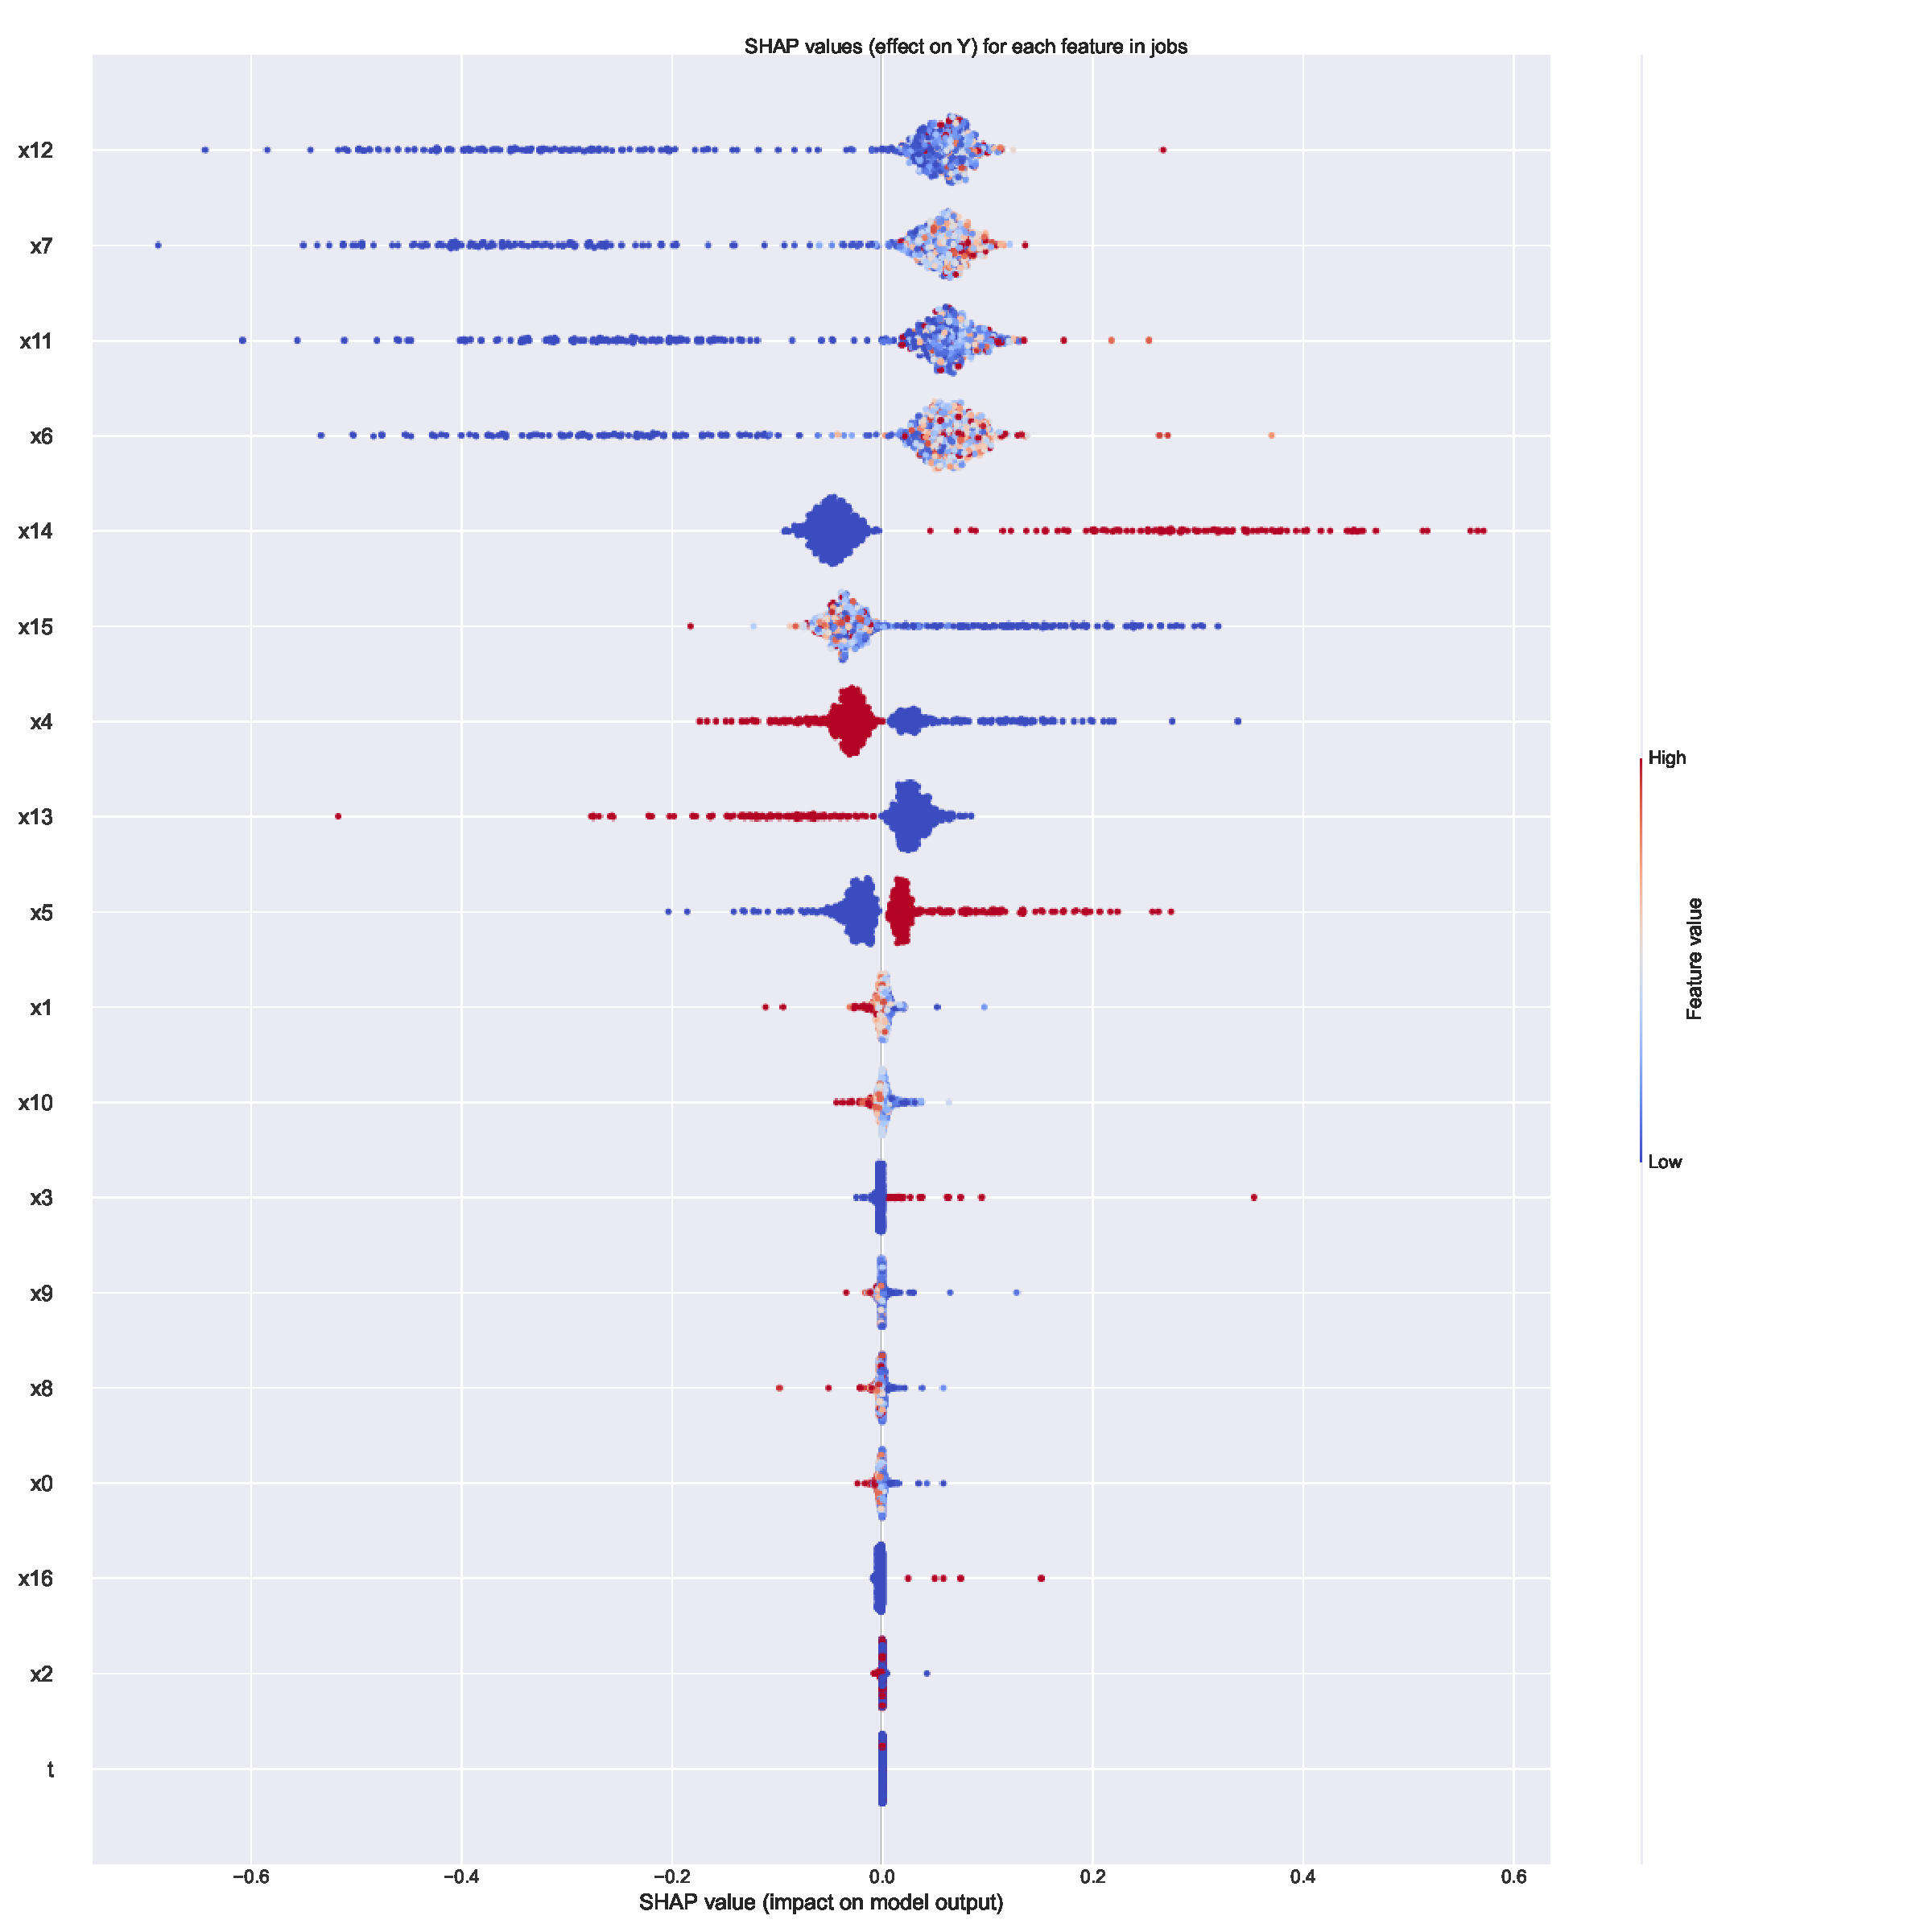
\includegraphics[width=1\linewidth]{project/assignment2/jobs/jobs SHAP values for sgd simple ipsw.pdf}
  \caption{Shapley values for the features as found by the JOBS Y|XT*IPSW SGD predictor}
  \label{fig:jobsSimpleIPSWB}
\end{subfigure}
\caption{Feature importances found by the JOBS Y|XT*IPSW learner}
\label{fig:jobsSimpleIPSW}
\justifying
\small
Seeing as the `T|X` predictor, shown in Figure \ref{fig:jobsIPSW}, was used to help fit this predictor,
it would have made sense if any of the other features relevant to the training of `T|X` would have been
considered to have had more of an impact for this estimator. However, the outcome of this is, for the
most part, functionally identical to the outcomes of \ref{fig:jobsSimple}.
\end{figure}

\FloatBarrier

\subsubsection{JOBS CATE estimator}

\FloatBarrier

The best CATE estimator for `JOBS` was the `CausalForestDML` estimator, with an
ATT\footnote{Absolute error in Average Treatment effect on the Treated} value of 0.349.
Once again, however, I suspect that it may not be fitted properly, due to the rather unexpected
shapley values and questionable tree interpretations (see Figures \ref{fig:jobsCATEcfA} and \ref{fig:jobsCATEcf}).


\begin{figure}[H]
\centering
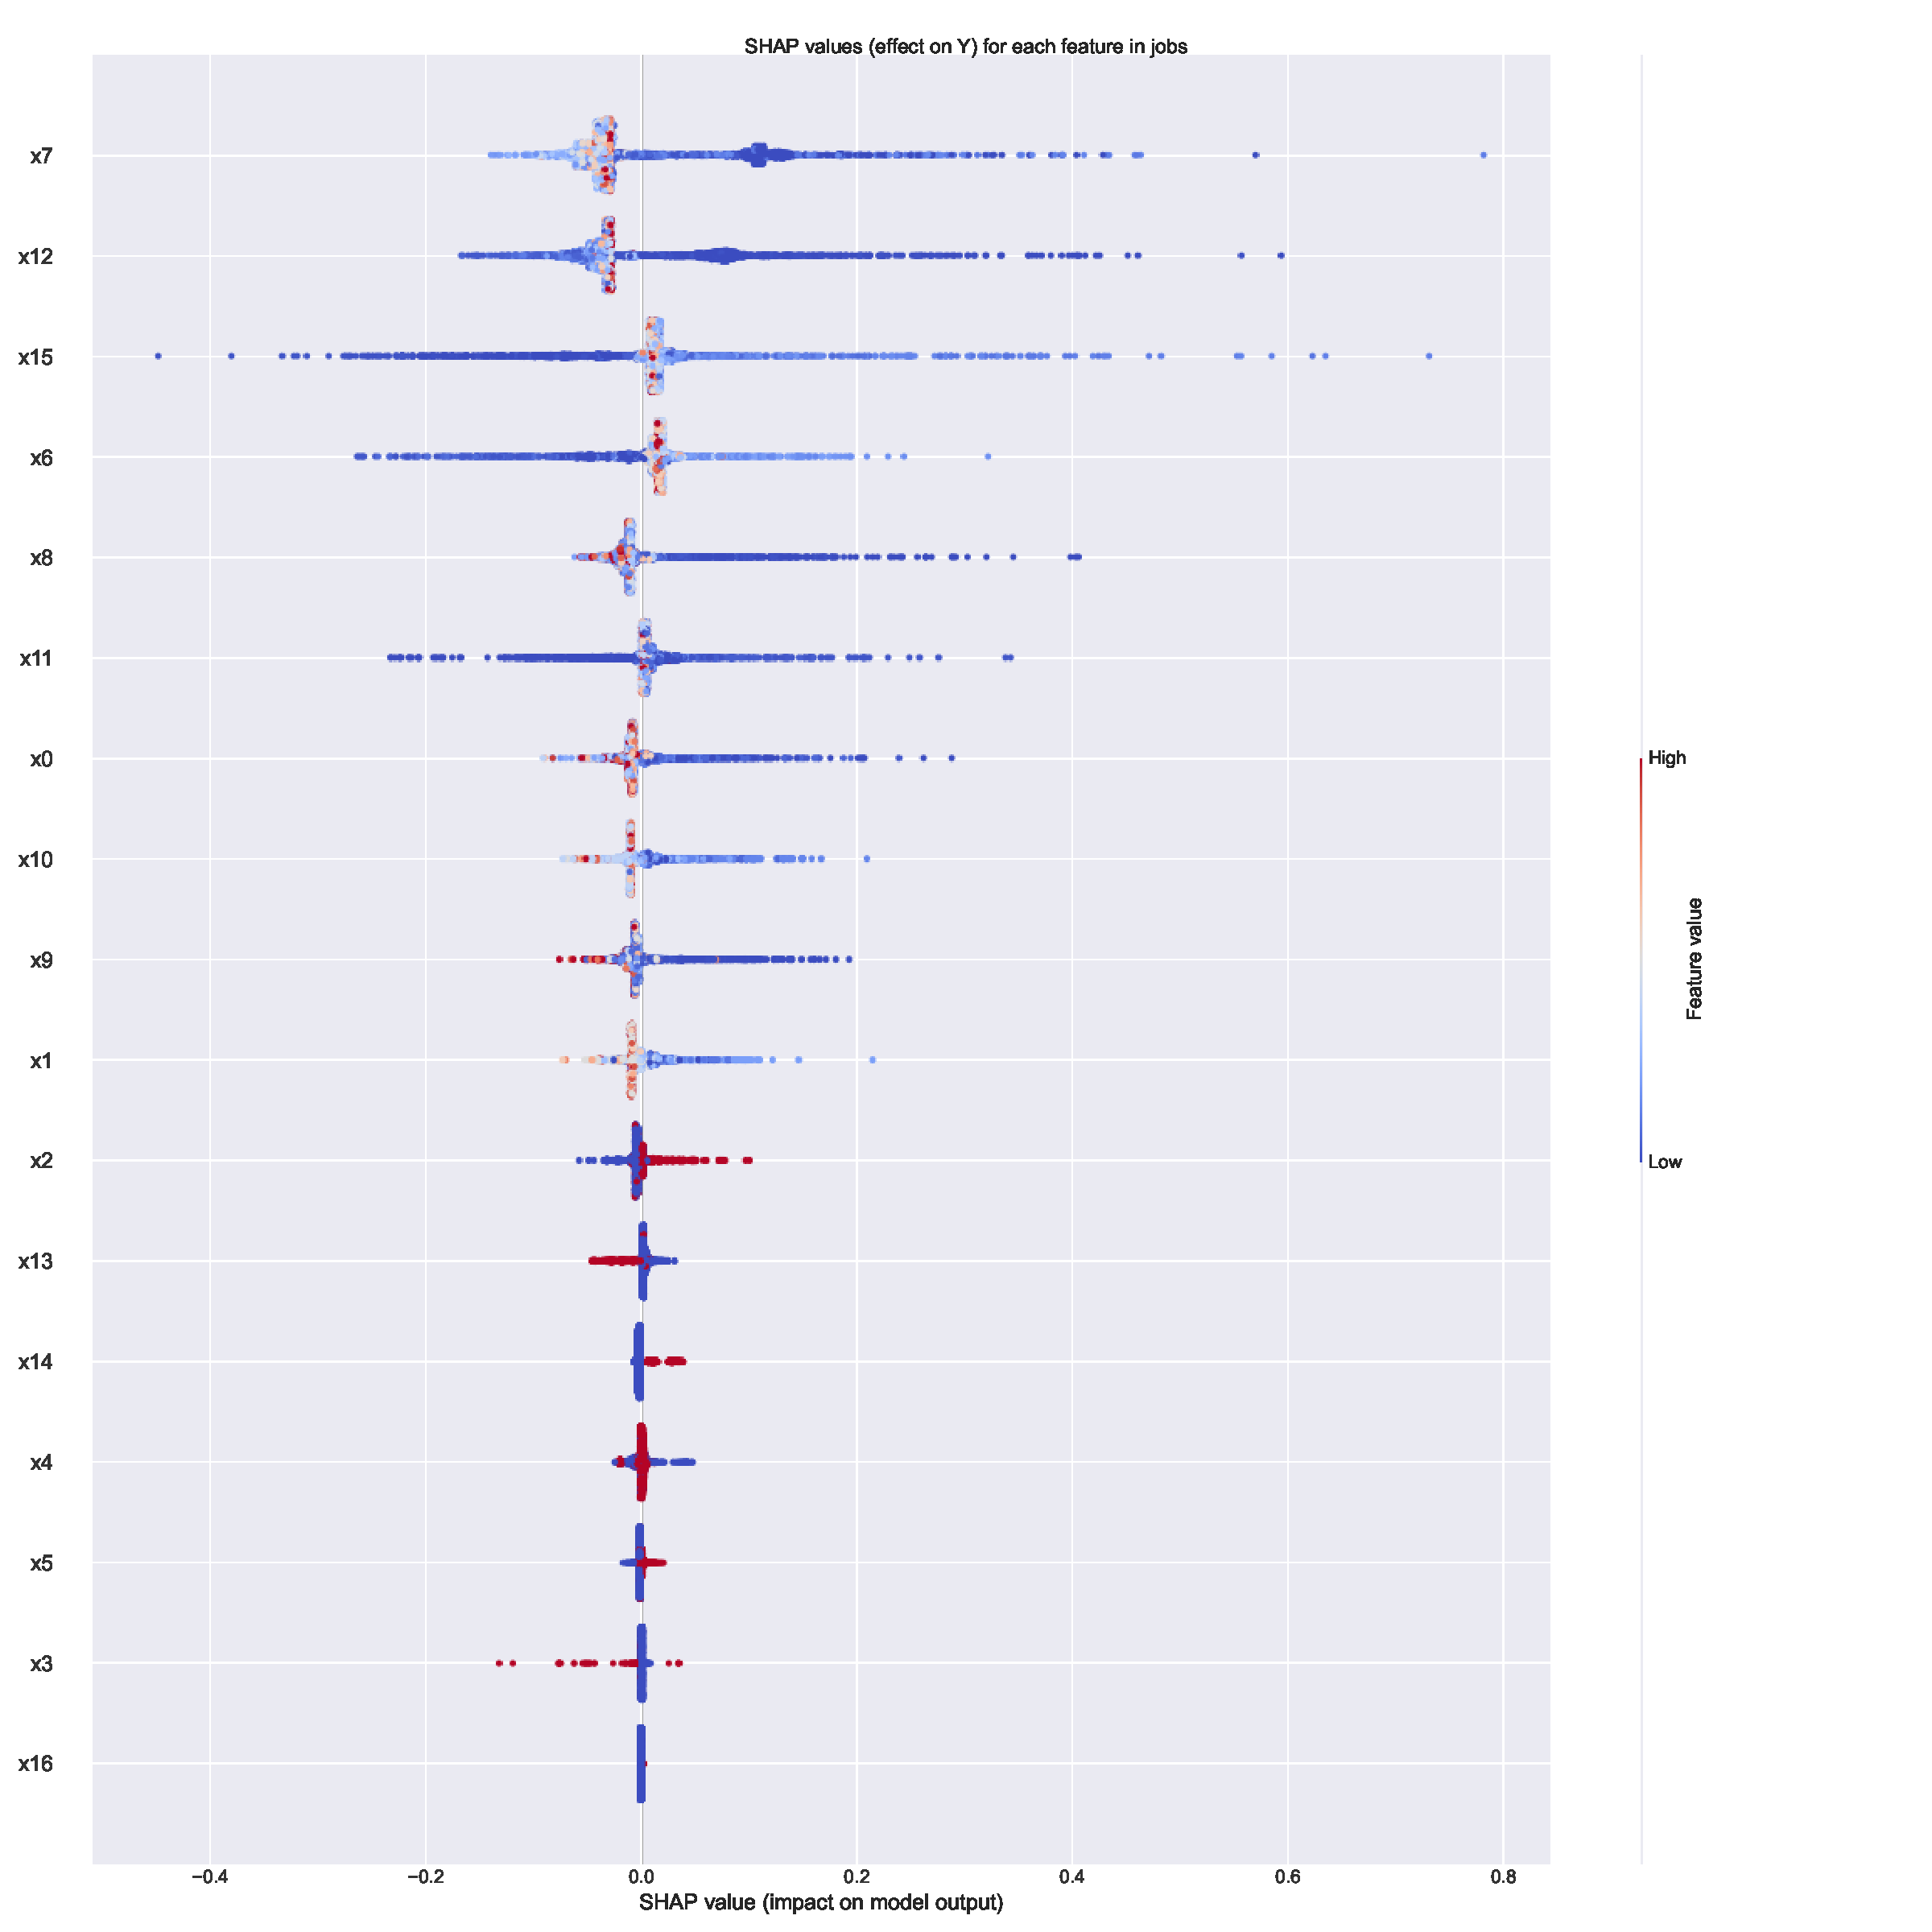
\includegraphics[width=1\linewidth]{project/assignment2/jobs/jobs SHAP values for Causal Forest.pdf}
\caption{Shapley values for the features in JOBS Causal Forest DML}
\label{fig:jobsCATEcfA}
\justifying
\small
These shapley values are somewhat unexpected, considering the lack of any resemblance they have
to the shapley values for the earlier predictors, and the seemingly nonsensical mixture of high values
and low values on either end of the `increase y` and `decrease y` sides of the chart, implying the
presence of a confounder, causing these seemingly completely arbitrary `y` outcomes for somewhat similar
`x` values.
However, from this graph, it appears that, if one wants to boost their chances of getting employed,
they need to ensure that their `x12`, `x0`, and `x8` isn't incredibly low (bringing that to the `+y` 
side), but to drastically lower one's `x15` and `x6` values (bringing those firmly into the `+y` side as well)
\end{figure}

\begin{figure}[H]
\centering
\begin{subfigure}{1\textwidth}
  \centering
  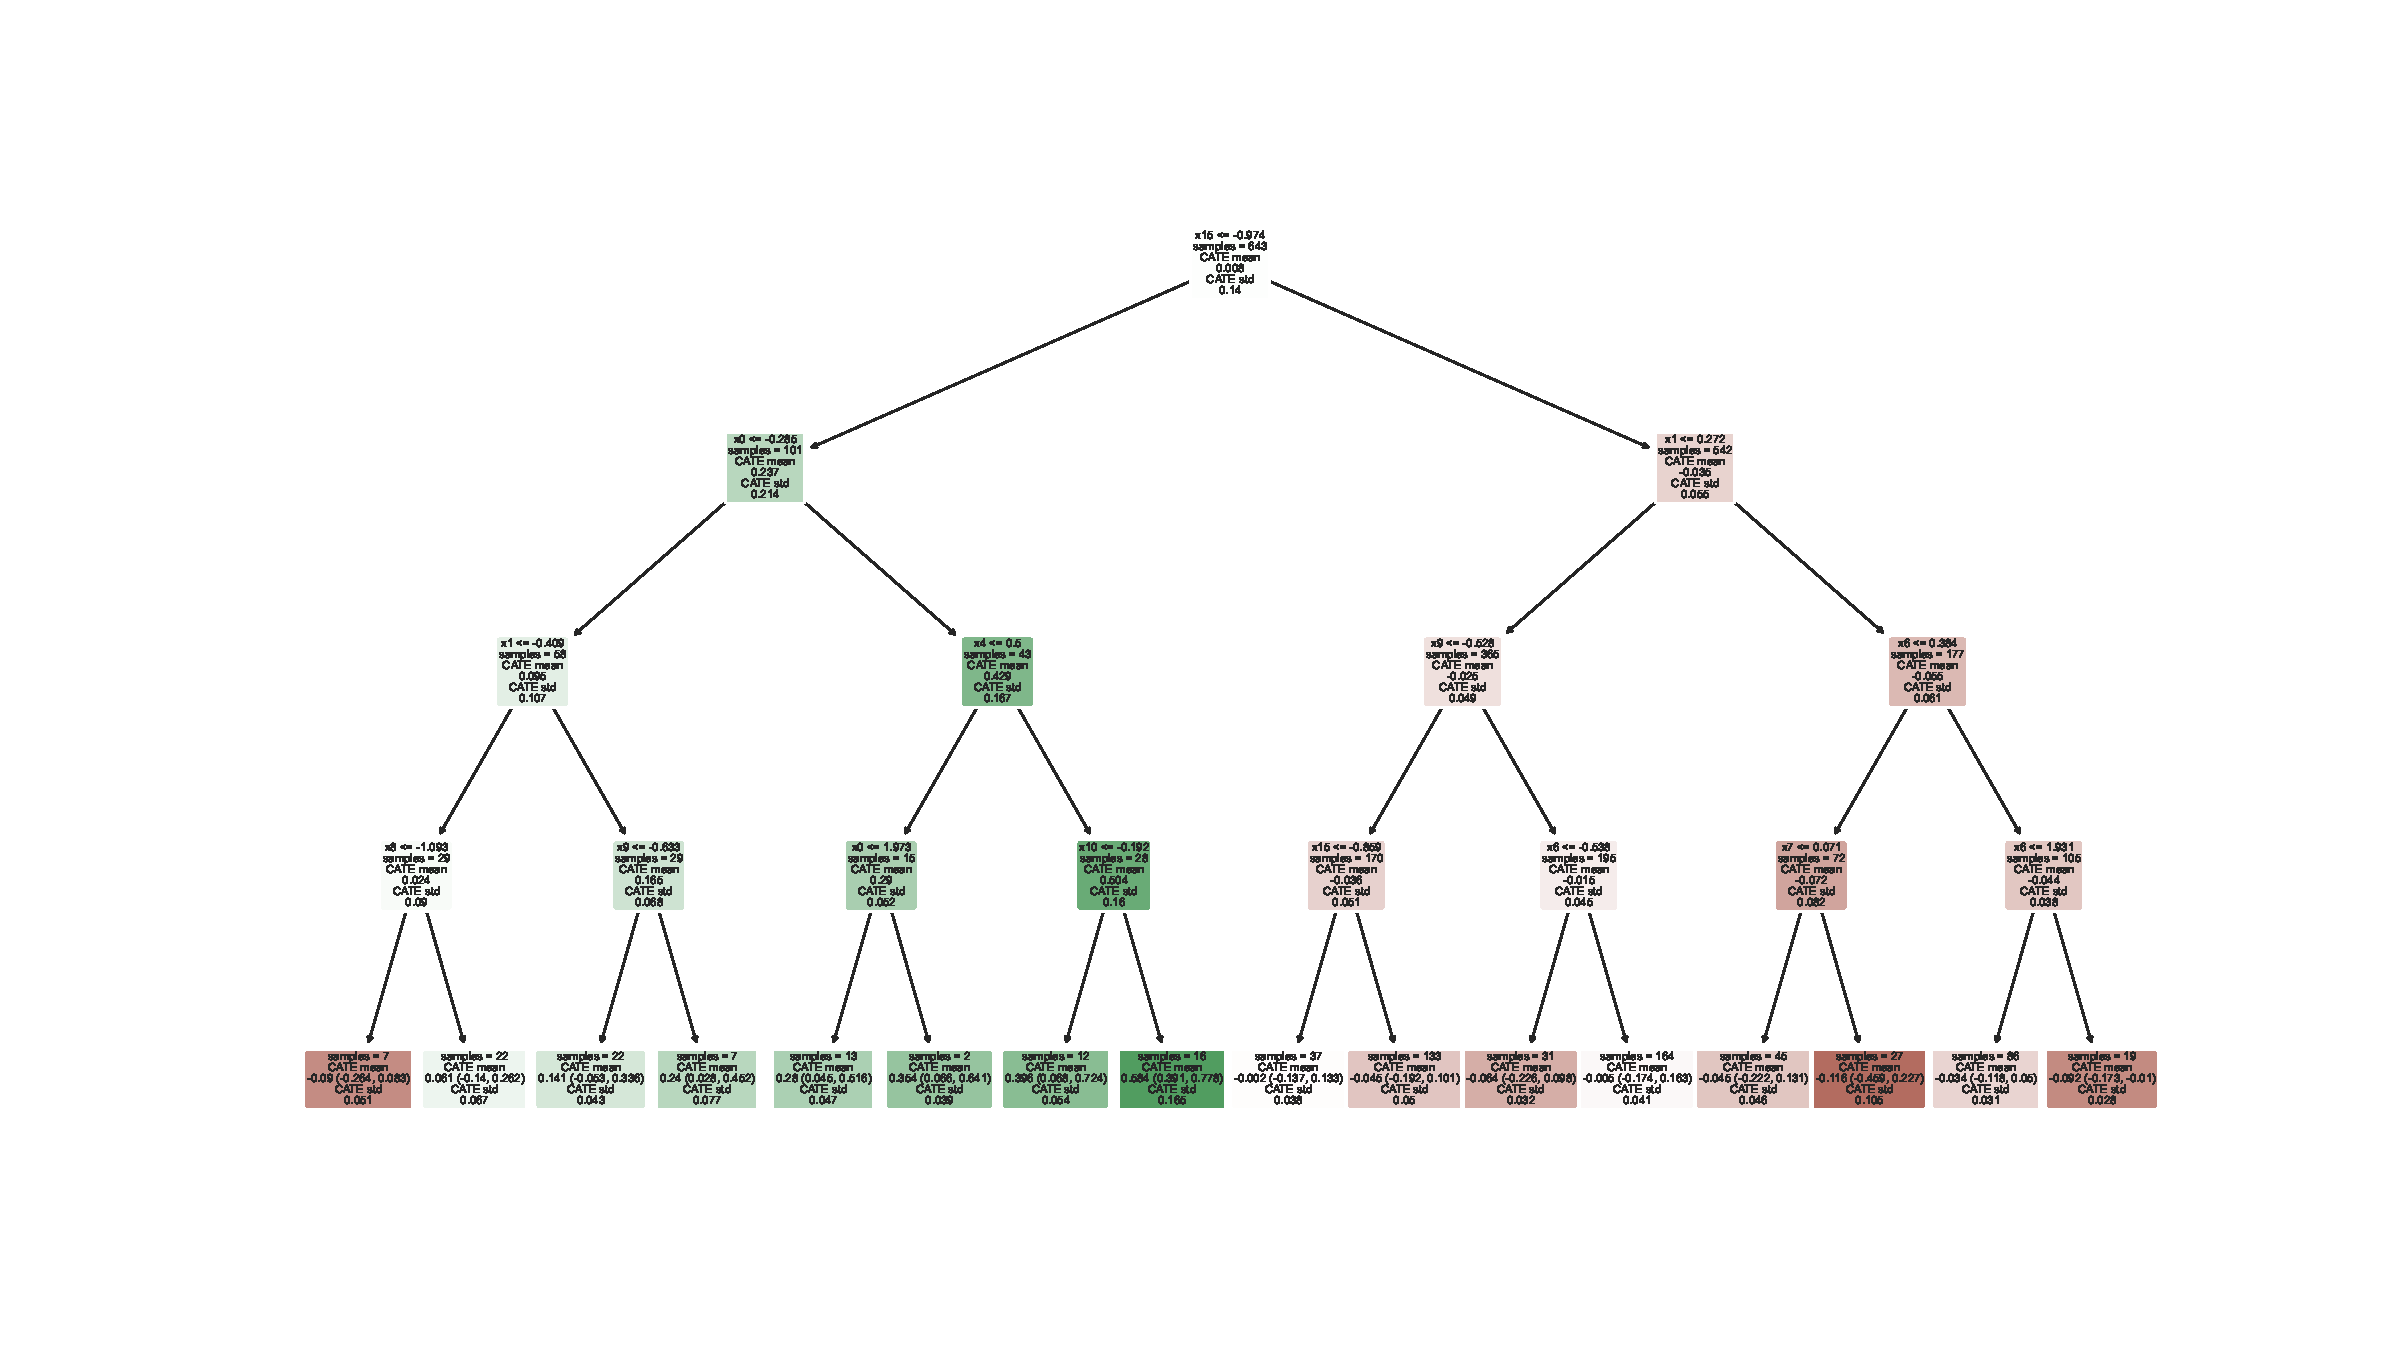
\includegraphics[width=1\linewidth]{project/assignment2/jobs/Causal Forest CATE tree.pdf}
  \caption{CATE interpreter tree for JOBS Causal Forest DML}
  \label{fig:jobsCATEcfB}
\end{subfigure}
\begin{subfigure}{1\textwidth}
  \centering
  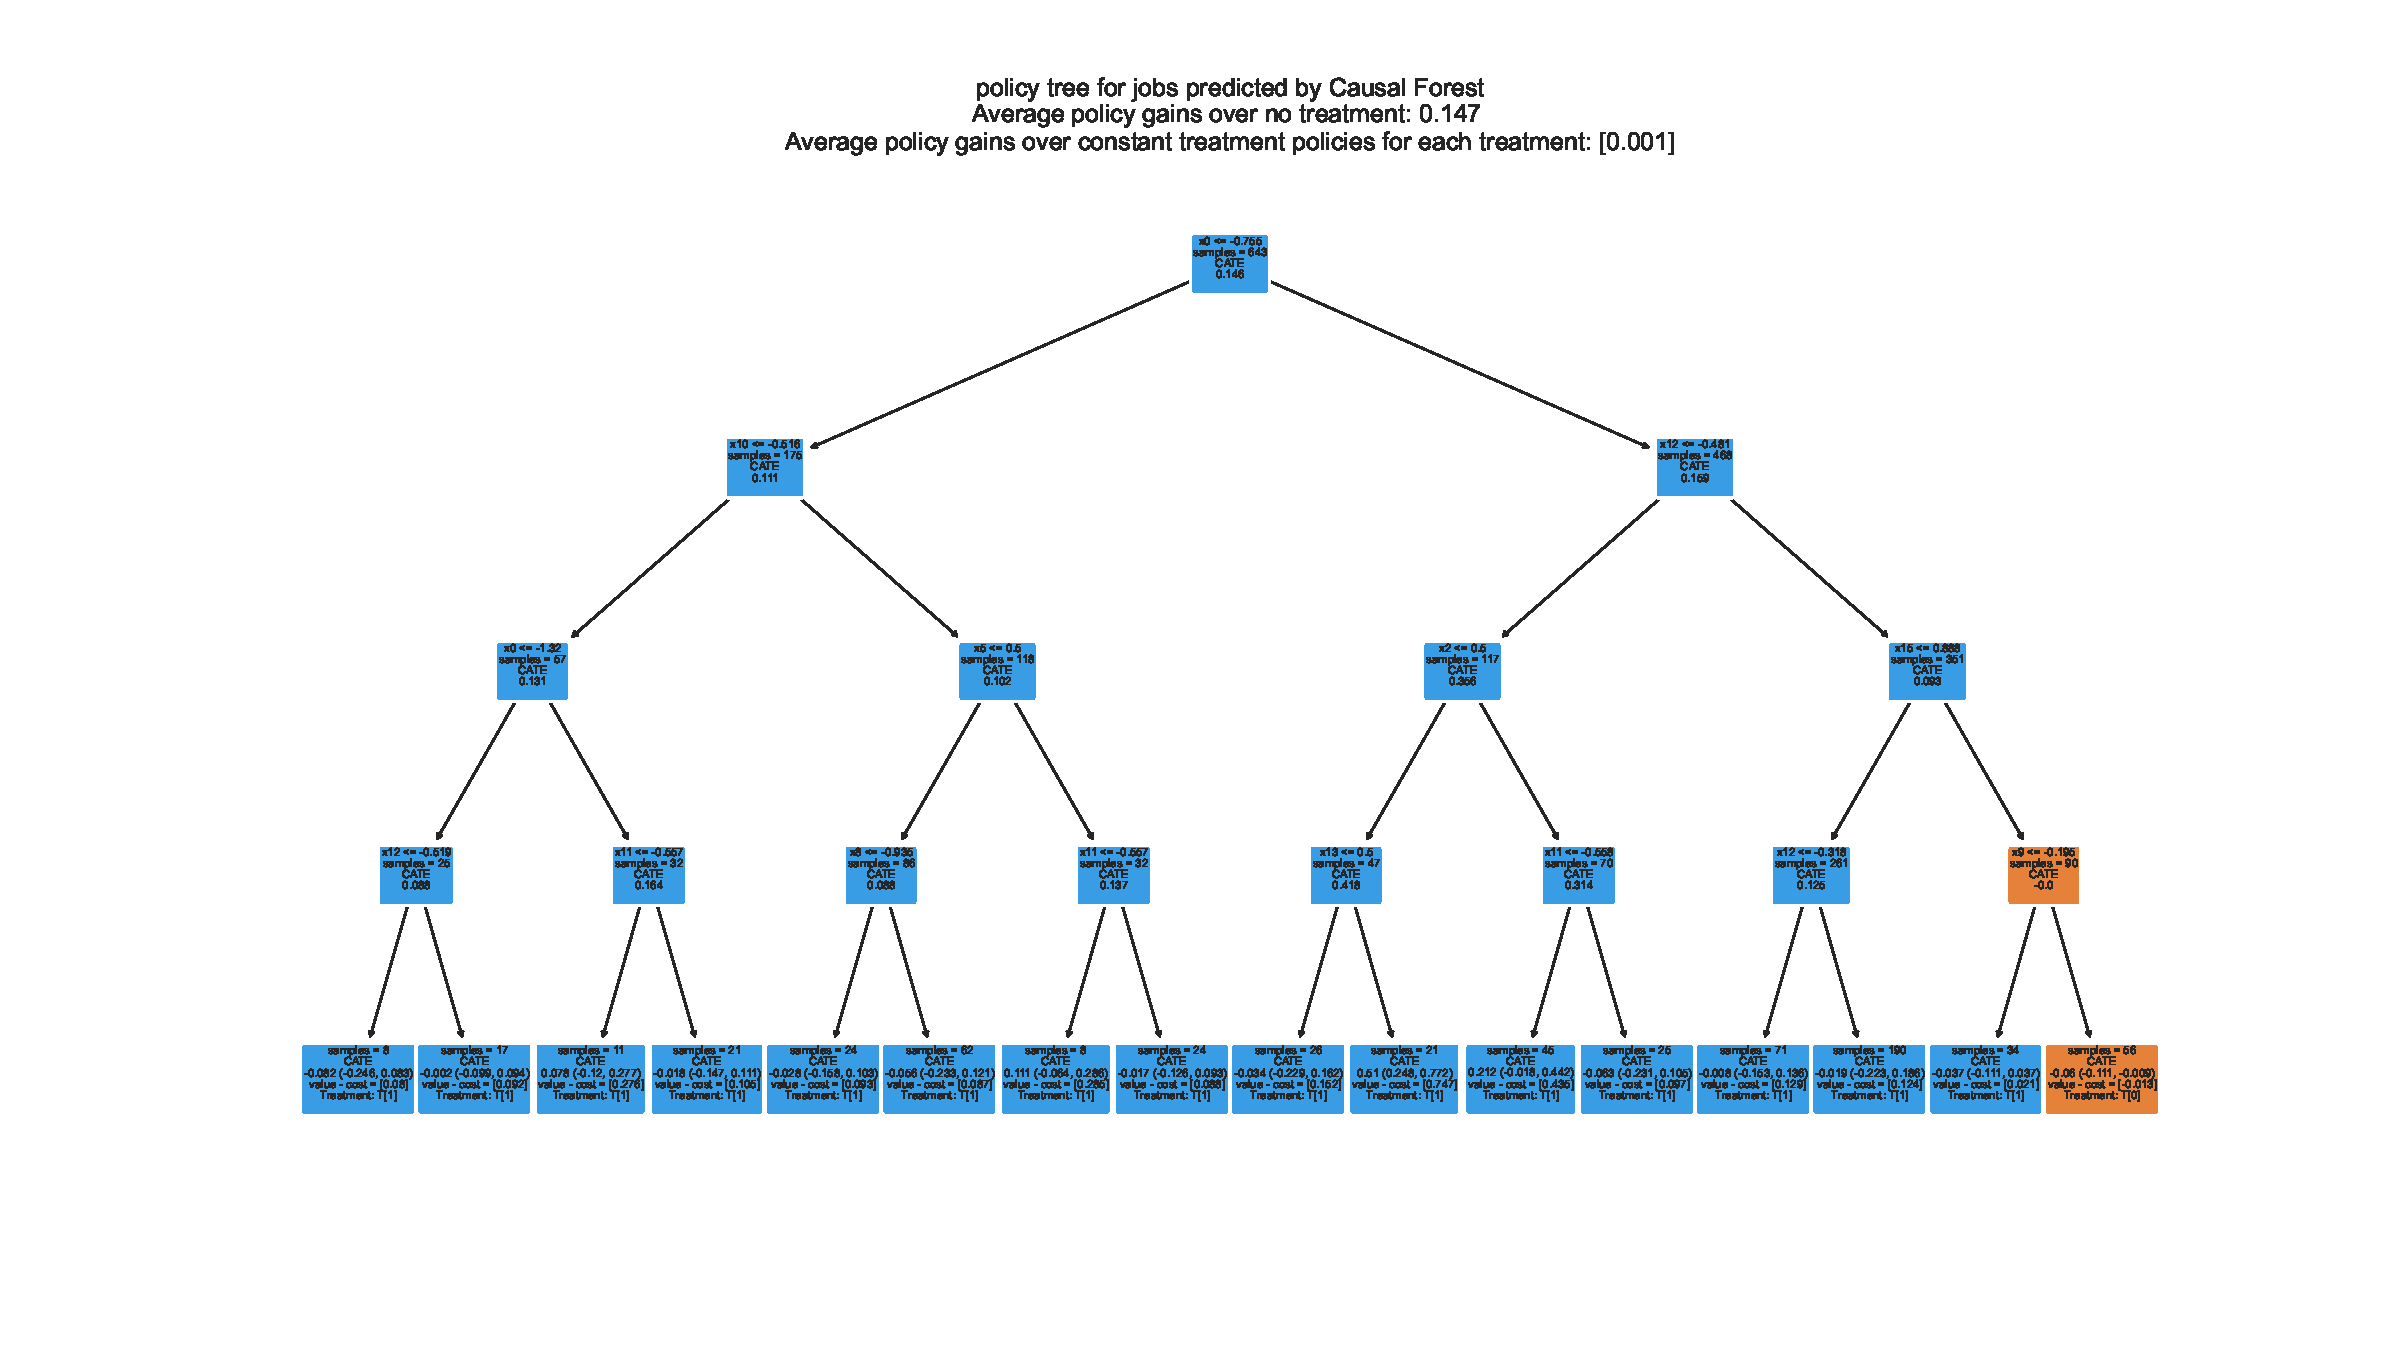
\includegraphics[width=1\linewidth]{project/assignment2/jobs/Causal Forest policy tree.pdf}
  \caption{Policy interpreter tree for JOBS Causal Forest DML}
  \label{fig:jobsCATEcfC}
\end{subfigure}
\caption{Interpreter trees for the JOBS Causal Forest DML}
\label{fig:jobsCATEcf}
\justifying
\small
These trees are interpretations of the inner workings of the Causal Forest DML CATE estimator (with these
trees being constructed by \cite{shaptree}).

These trees both appear to suffer from poor fitting. The CATE tree in \ref{fig:ihdpCATEcfB} appears
mostly normal (with a somewhat helpful indicator of the conditions where the treatment may have a 
negative effect on the treated), however, the projections of CATE values far outside of the true
`y` range of `0-1` indicates that the CATE prediction model may be somewhat underfit (making assumptions
of CATE values that may not actually be possible). Despite this, it does still provide an indication
of which samples might respond negatively to treatment.

The policy tree in \ref{fig:ihdpCATEcfC} is either underfit,  rather poorly-thought out, or both (or I'm
just misreading it), due to how it advises treating individuals with a seemingly negative CATE (and
therefore would probably not benefit from the treatment), instead of going further to divide the leaf
nodes further into clear 'treat' or 'don't treat' leaves.
\end{figure}

\FloatBarrier


\section{Conclusions}


This project has not been a success. Neither investigation produced any meaningful results,
mostly due to the poorly-thought out methodology I used to approach this task.

Whilst the program structure used may, in theory, be applicable to a normal machine learning problem,
and the requirements of having simple estimators, IPSW estimators, Simple+IPSW weighting estimators,
and CATE estimators were met, the initial aims for this project were not met.
I spent too long working out the particular program architecture used to get from the start to the point
where the causal inference was supposed to happen, and, only after I had finally ran everything from the
simple estimators to the CATE estimators (with all the graphs produced along the way), I realized
that I had completely neglected to consider how to extract the actual answers from the data.

Certain aspects of my approach reeked of 'seemed like a good idea at the time', prompting further
delays to reaching that point of realization. For example, I made a major blunder with the training
set/test set. Whilst, yes, I did keep the full training data and the validation data completely distinct,
and did not use any of the validation data (or the counterfactual data) within the training process,
(relying on 10-fold cross validation for the training), I used a single validation set repeatedly for all
of the validation (including the validation when working out which model was the 'best' and worthy of
being used for the later modelling stages), meaning that the produced models were effectively indirectly
trained on the validation set. Furthermore, the usage of passing the seed, `42`, as a \bold{number} to
every `scikit-learn` method which could be given a seed, instead of passing a `RandomState` with a seed
of 42 down the callstack, may have lead to some stagnation in the models, such as by how all of the
simple models were trained on the exact same sequence of KFold indices every time. Of course, there are
still merits to passing in a number instead when consistency is important for reproducability of results,
but defaulting to a RandomState from a specified start position each time would still be reproducable.

On a less negative note, the `.py` files in `assignment.a2\_utils` are somewhat reusable (with it being
somewhat feasible for some of these classes to be adapted to more general data science tasks, potentially
allowing some time to be saved with setting up some of the code for these tasks). However, the glaring
omission of anything that can actually be used to perform any meaningful causal analysis will need to
be addressed.

To summarize, due to my poor approach to and mismanagement of my work on this task, the only conclusion
I can make is that I have not made any findings significant enough to warrant any meaningful conclusions.


\appendix
\section{Appendix: Further visualizations of note}\label{appendix:graphs}

These are some supplementary figures, not intended to replace the main content,
but merely to supplement them.

\subsection{IHDP CATE}


\FloatBarrier

\begin{figure}[H]
\centering
    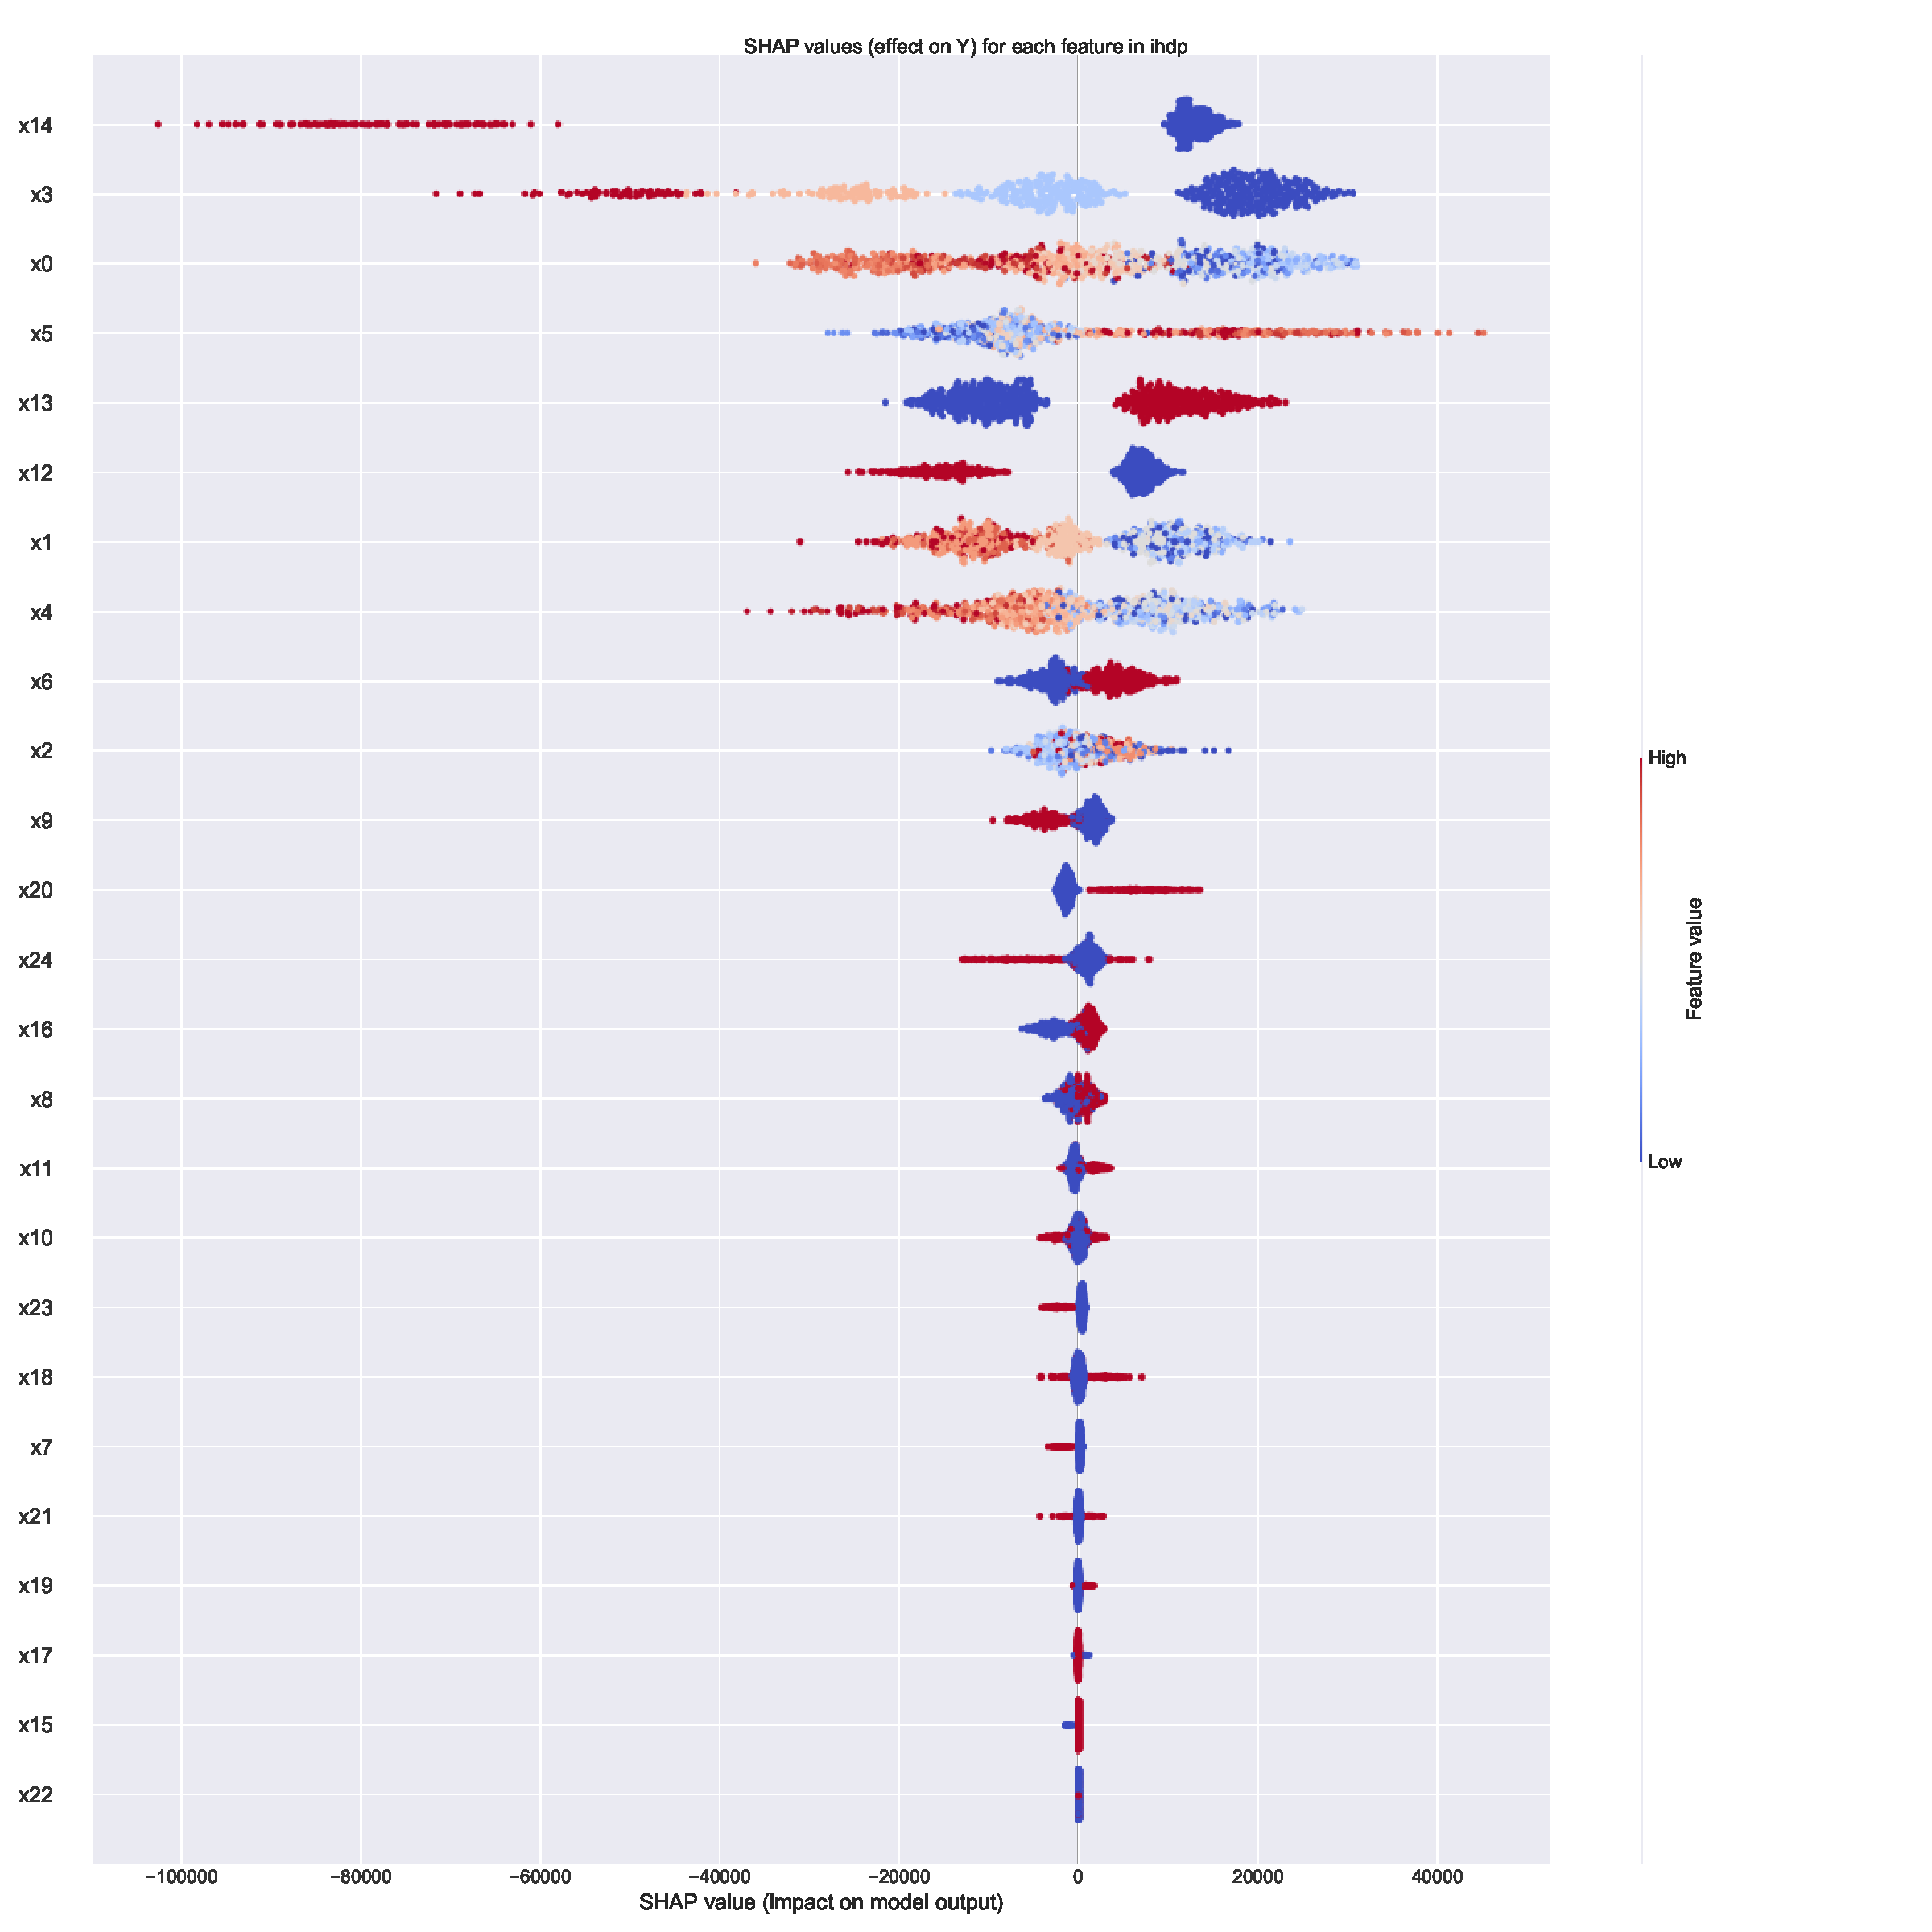
\includegraphics[width=1\textwidth]{project/assignment2/ihdp/ihdp SHAP values for Forest DR Learner.pdf}
    \caption{
        \label{fig:ihdpForestDRShap}Shapley values for the IHDP ForestDR CATE estimator
    }
\justifying
\small
These shapley values for the ForestDR learner appear to more closely resemble what one would
anticipate to see from the CATE estimators for IHDP, considering the inputs found along the way,
significantly moreso than the CausalForestDML results, visible in Figure \ref{fig:ihdpCATEcf}
Considering the fact that the Y estimators (somewhat illustrated by Figures  \ref{fig:ihdpSimple} and \ref{fig:ihdpSimpleIPSW}) granted some semblance of importance to x14, it makes sense that it might be
seen as having some potentially drastic impact on the predictions made by this estimator, which uses
those estimators as part of its inputs. Additionally, x5 (also identified as important by those predictors) is also shown as having relatively high importance. Furthermore, x3 (indicated as a
key contributor towards `t` by the estimator illustrated in Figure \ref{fig:ihdpIPSW}) is also
shown as being rather important in this estimator, as expected.

However, in practice, these shapley values are from an estimator with a PEHE (Precision of Estimation
of Heterogeneous Treatment Effects) value of 68332.93913561162.

PEHE is supposed to be minimized.

Which is another way of saying 'these shapley values are utterly incorrect in practice'. This either
means that the learner itself was poorly fitted (garbage-in-garbage-out), or it could mean that
there was a rather large unknown confounder interfering with the outputs of this learner, but,
considering the rather underfit learners which lead up to this point, it is most likely the former
(garbage-in-garbage-out), not the latter.

\end{figure}


\FloatBarrier



\quoteOFF
\printbibliography


\end{document}